% book
\documentclass[paper=6in:9in,pagesize=pdftex,headinclude=on,footinclude=on]{scrbook}
\areaset[0.50in]{4.5in}{8in}
\renewcommand*{\chapterformat}{%
\fontsize{80}{88}\selectfont\thechapter\autodot\enskip}
\renewcommand{\footnotesize}{\small}

% PDF
%\documentclass[a4paper,12pt,oneside,openany]{book}

% ebook PDF
%\documentclass[a5paper,12pt,ebook,oneside,openany]{book}

\usepackage[utf8]{inputenc}
\usepackage{sectsty} % Change title formatting
\usepackage{graphicx} % \includegraphics
\usepackage{color} % \color
\usepackage{hyperref} % \url
\usepackage{breakurl} % Fixes some "Overfull \hbox" errors in \url
\usepackage{pgfplots} % Graphing plots
\usetikzlibrary{plotmarks}
\usepackage[superscript]{cite} % Changes bibliography citations to use superscript
\usepackage{fancyhdr}

% Page style config
\pagestyle{fancy}
\fancyhf{}
\fancyfoot[LE,RO]{\thepage}
\renewcommand{\headrulewidth}{0pt}
\renewcommand{\footrulewidth}{0pt}

\title{Freedom Beckons}
\author{Marshall Mason}

\pgfplotsset{compat=1.11} % Recommended by pgfplots manual
\setlength{\parskip}{0pt} % Prevent huge spaces between paragraphs
\setcounter{secnumdepth}{0} % Turns off numbering for sections
\chapterfont{\centering\fontfamily{pzc}\selectfont} % Change title formatting
\renewcommand*{\thefootnote}{\fnsymbol{footnote}} % Use symbols for footnotes

\begin{document}
\frontmatter
\chapter{Note to the reader}
This book was not written with the intention of subsidizing my own financial independence. My only goal in writing this book is to further the cause of freedom and help people find more freedom in their lives. Therefore, all net proceeds from this book will be donated to \textbf{Oxfam} and \textbf{Amnesty International}.

I also want the book itself to be as free as possible. I don't expect readers to spend money for a book that urges them to spend less money. Aside from the obvious contradiction, this also limits its readership to those with money to spare, when the whole point is to maximize freedom for all. I also want its readers to do with it as they feel inspired to do, to modify it, redistribute it, or share it with friends. Therefore, it is licensed under \textbf{Creative Commons} and available as a free download at \textbf{www.freedombeckons.com}.

\includegraphics[bb=-125 40 0 0]{cc.png}
% First number: higher number moves left
% Second number: higher number moves down
% Third number: ignored
% Fourth number: higher number moves down

\let\cleardoublepage\clearpage % Prevents the extra page after every chapter
\tableofcontents
\chapter{Preface}
\fancyhead[CO,CE]{\emph{Preface}}
I flunked nearly every class in school. I intentionally caused trouble for most of my teachers. I skipped classes every chance I had. I was suspended from school almost as often as I was in attendance. My parents and teachers assumed I was a ``bad kid'' who might shape up with enough discipline. They figured I wouldn't make it to graduation. Certainly no one dreamed I'd retire in my early 30's. Looking back, I feel like my whole life was leading up to it.

Many people ask me how I did it, and they seriously think I can give them a one-sentence answer. A lot went into this goal. It was a labor of love. It had just as much to do with passion and commitment as with investing and frugality. Motivation is everything for such a huge life dream as this, so before I talk about \emph{how} I did it, I want to explain \emph{why} I did it.

Defiance wasn't in my nature. I was actually very cooperative as a child. I instinctively wanted to do the right thing. I had a lot of energy and curiosity. I would latch onto adults and ask them an endless stream of questions. I had an intuitive sense of ethics and fairness. One of my earliest memories is a feeling of terror when I discovered I'd forgotten to pay for a five cent piece of bubble gum at the store. I walked all the way back to apologize and pay for it.

I've always remembered my preschool teacher as one of the kindest people in the world. She radiated love and embodied compassion. I felt safe and happy with her. What I remember most distinctly was how overjoyed she was. She absolutely adored kids. This is the kind of teacher kids should be accustomed to, but I'm grateful to have had this one.

My parents were fairly invested in the family. They didn't spoil us, but we had lavish Christmases. We went on interesting summer vacations every year. We ate dinner as a family every night. They were usually very warm and caring. I was a cute kid with a lot of energy, and I often felt adored by everyone.

But my life turned very ugly for me, early in my childhood. Things got very bad, and then they got worse.

My father seemed to have two different personalities---one that loved me and one that hated me. Whenever I was being punished, I felt hated. Because of my cooperative nature, I've always found punishment very confusing. It never seemed to fit the crime. I usually didn't even understand what crimes I'd committed, like the time he grounded me for not making my bed, until he realized he'd never actually taught me how. Here's a pattern that repeated in my home: my brother would hit me, and I'd cry. Then my father would come and hit me for crying. He'd send me to my room for the rest of the day, where I would continue sobbing for hours, and be ignored.

This happened often, but one time in particular has always stuck with me. It was earlier in the day, so I was grounded to my room longer than usual. I cried endlessly, all day, and well into the night. My stomach was growling, and I could hear my family sitting down for dinner without me. I wailed even louder, and started yelling that I was hungry. I was still crying when I heard dishes being put away. I told myself I had to keep crying, because if I stopped, they might forget I was there---my pain would become invisible. But it didn't work. The lights were turned off, and eventually all I could hear was the television.

Then I realized something tragic: \emph{nobody cares.} I looked around the room, taking stock of how I felt at that moment. I took a snapshot in my mind. I thought about how lonely and angry I was. I promised myself that I would never forget that moment, or what it was like to be a kid, to feel so trapped and helpless, to be so powerless over my own life. I promised myself that, once I was older, I would never treat kids the way I was treated, and would get to the bottom of this injustice. Of course, I couldn't have articulated it like that at the time, but that was the essence of the promise. For the rest of my life, I never forgot that night, and over time, the promise I made to myself blossomed into an obsession with freedom.

School was no better for me. Ms. W was a monster masquerading as a fifth grade teacher. She would yell at me, I would cry, and then she'd call me a cry baby. She often told me I was stupid, as if reminding me just in case I'd forgotten. When I was sniffling a lot from allergic reactions, she said I was gross. I tried to stop sniffling, but I didn't know how. I figured it was because I was stupid. What I remember most vividly was when she brought me into the bathroom where no one else could hear her, and yelled at me as I cowered in the stall and cried. I just sobbed uncontrollably while she yelled at me to stop crying. ``Grow up! Only babies cry!'' she would yell. I tried to tell my mother about this, but she didn't believe me. The year I spent with this teacher changed me forever and completely. My attitude toward authority figures was transformed by this experience.

My sixth grade teacher found me extremely difficult to work with, and she was visibly frustrated. It seemed impossible to motivate me. She punished me a lot, sometimes she pleaded, and sometimes she tried pep talks. She told me I had a lot of potential, if only I would apply myself. When I started junior high, I made a sincere attempt to be a good kid and a good student, but met with limited success.

I tried hardest in Mr. G's class, which had a strict and detailed system for measuring and boasting success. From the very first day, the kids in the front were obviously favored, and seemed to breeze through the class with lots of attention from the teacher. The smart kids seemed like an exclusive, elite club, a higher caste that I was simply not born into. I sat in the back with the other misfits. I was obviously one of the stupid kids. No matter how hard I tried, I couldn't break out of my caste.

My parents had become increasingly distant around this time. They separated, and nearly divorced, but changed their minds after many trying months. They stayed together after this, but everything changed. They were no longer so invested in the family. No more family dinners. No more summer vacations. No more weekend outings with my father. We moved across the country, and they started a business together. I didn't see them much anymore, and their influence in my life mostly disappeared at this point. They started to feel like strangers whose task in life was to punish me. I thought of them more as prison wardens than parents.

All of my efforts in school felt wasted. There was so little incentive to work hard. I didn't get anything for it, just a letter grade on a piece of paper, which was meaningless to me. Adults seemed to think it was important, so I figured I could use that grade to finally earn the respect of my parents and teachers, but that wasn't forthcoming, despite my best efforts. Besides, I resented that I had to earn their approval by doing these tricks for them. I simply gave up trying.

This was a point in history when the schools had become preoccupied with self-esteem, a contentious obsession that not everyone agreed with. All students were required to be evaluated by a psychologist. The man I met with asked me to give him an analogy of how I felt about myself. I told him I felt like a piece of trash in a trash can that someone hits with their car. He found this disturbing, and decided to schedule an appointment with an on-campus therapist. When I met with her, I felt very safe. I told her everything about fifth grade. She listened to me and believed me. It was such a relief to find an adult I could trust, someone I could talk to whenever I felt lost or scared.

A couple days later, I was called out of class to the principal's office. I had no idea what provoked this, so I was fairly alarmed. The principal sat me down and closed the door. He alternately yelled and hissed at me about how I was privileged and whiny, that I was taking advantage of the system. I had no idea what he was talking about. I just sat there shaking as he laid into me. This lasted for the remainder of the class period. When the bell rang and I was excused, I went directly to the therapist's office, still shaking from the verbal assault. I started telling her what had happened, but she stopped me short. She said that I couldn't meet with her anymore, and she suggested I just try to move on. I felt incredibly betrayed, and more alone than ever.

The lesson from school that really stuck with me was that there are smart kids and there are stupid kids, and no matter how hard I tried, I would always be stupid. Learning seemed to be something that only happens in school, a dreadful, boring process to be avoided at all costs. I also learned that adults are not to be trusted, and they will usually betray me, even when they seemed like my friend.

School felt like a jail, which seemed strange in a country that boasts about freedom and democracy. There was a pecking order of good kids and bad kids, with systems in place for disciplining those who got out of line. I was confined and legally forced to obey rules made by arbitrary authorities, joylessly doing work with no incentive. I was punished for my disobedience. I had very little say in my own well-being and destiny. I was legally forced to attend this institution, and could literally be jailed for refusing. I needed to ask for permission to do even the most basic and private of functions. I was under constant surveillance. A strict schedule was facilitated by bells ringing throughout the day to shuffle me off to the next authority figure, who did as they pleased.

I believed, but could not yet articulate, that no one, anywhere, should stand for such a totalitarian regime. I couldn't fathom adults tolerating this kind of oppression, but they seemed to believe this was the appropriate setting for young people, as if it were some kind of boot camp for a lifetime of compliance and obedience as adults. I didn't see what my youth had to do with it. It seemed very much like age discrimination, and defiance was my only reasonable and ethical reaction.

By high school, I became more skilled and intentional in my defiance. I didn't just give up trying---my goal was to be the anti-student. The teachers wanted cooperative kids who studied and got good grades, so I did the exact opposite. I tried to make their lives as miserable as I could and get the worst possible grades. That way, they would have no power over me, and I made sure they knew that.

One teacher eventually got to the point that she could just look at me when I came in and see that I was ready for battle. She could read it on my face, and would make a preemptive strike, sending me to the principal's office before I even did or said anything. One day she asked if I intended to do this every day, and I said that I absolutely did, so we agreed that I'd just come in each day to pick up my referral slip.

Another teacher had a point system for determining grades, and misbehaving had the effect of deducting points, which I found very exciting. Here was a whole new tool in my quest for the worst possible grades. Before this, the worst I could get was a zero, but this was the first time I could get a negative grade! Unfortunately, he caught onto my game, and refused to deduct my points, no matter how poorly I behaved, so I never reached this crowning achievement.

My parents continued trying to punish me for my increasingly defiant behavior. They sought more creative punishments, and were distraught by how I just seemed to get worse the more they punished me. One day, they tried taking away my guitar, my only solace, to which I responded by not speaking to them aside from the occasional ``fuck you.'' After weeks of this, they took me to a family therapist, to whom I would continue to say my usual epithet. Finally, the therapist seemed to give up, and just started talking about himself, like the problems he was having with his computer. This was something I loved talking about, so I started to open up, and we had a great conversation. When my parents came to pick me up, he told them, ``your son is fine. He just needs his guitar back.''\footnote{I discovered this recently, which explains my entire adolescence: ``Confused and bewildered parents mistakenly hope that punishment will \emph{eventually} bring results, without realizing that they are actually getting nowhere with their methods. The use of punishment only helps the child to develop a greater power of resistance and defiance.'' - Rudolf Dreikurs, M.D.}

I did need my guitar back, but I wasn't fine. I was becoming extremely depressed. I felt desperately lonely, alienated, and unloved. My life was turning into a failure. I thought I was stupid and incapable of doing anything but making life hard for people. I had few friends, and my peers were cruel in their bullying and teasing. The only option that made any sense was suicide. I figured, maybe then people would take me seriously. They'd regret how they treated me. My life would be over, I would no longer be suffering, and everyone would blame themselves for it. Win-win.

I didn't go through with it because I knew there was one thing that I still loved in life: music. If there was one thing, then it was possible there would be more in the future. I wondered if I could hang onto music as my life preserver to get me through in the meantime, and I knew that I could. Music became my salvation and my only reason for living.

I transferred to a continuation school, where the teachers were more accustomed to kids like me. The counselor at this school was none other than Mr. G, my teacher from junior high, who must have thought his quirky brand of tough love was a great service to this wretched band of misfits, gang bangers, pregnant teens, and drug addicts. I had fewer opportunities to fight with the teachers, partly because some of the teachers treated the kids with respect and decency, and partly because most of the learning at this school was self-directed.

We worked at our own pace, and graduated as soon as we completed our high school requirements, which could be earlier or later than our usual graduation dates. The harder we worked, the sooner we graduated. Or we could do nothing at all, and never graduate. It was up to each of us how much or little we wanted to do. We were rarely nagged, and there was no attempt to discipline us for not being ``on task.'' This came as a great relief to me. This system gave me a real incentive to work, and less incentive to irritate the teachers.

However, I still wasn't very motivated, and was frequently suspended from school for increasingly controversial reasons. One time, the police were even called in, but I think that was just theater. My parents seemed to give up on me by this point, and only complained about the constant nuisance of being called at work to tell them that I was suspended yet again. My mother said she dreaded picking up the phone because the school was always calling her with more bad news.

Then I met Mrs. Adams.

She didn't seem very responsive to my misbehavior. She didn't get upset with me, or try to punish me. So I just goofed off and waited for the class to be over. When she gave me a math test, I discovered she'd given me the teacher's edition. My joyous defiance was rekindled once more as I copied all the answers from the back of the book and handed it in.

She thanked me and looked it over. I was quite proud of myself for my little stunt, and stood there confidently, knowing every answer would be correct. She asked if I could show her how I did one of the math problems. I looked at it and said, ``um, I forget.'' I knew I was busted. I was prepared to head to the principal's office for yet another suspension.

She said, ``okay, well, let me show you how I do it,'' and asked me to take a seat. Reluctantly, I sat down and watched as she worked out the math problem. Then she started on the next one, explaining what she was doing as she went along. I sat there uncomfortably, trying to figure out what she wanted from me, whether I was on my way to see the principal, or if I could go back to my desk. But she just kept working on math problems, and didn't seem to be trying to do anything else, so I just sat there and watched.

After a while of this, I was surprised that I was actually understanding what she was doing, and got the urge to try it myself, just to see if I could. I still wanted to be defiant, and I certainly didn't want to \emph{learn} anything, but I couldn't help it. She was hogging all the fun. I asked if I could try one. ``Sure,'' she said, and watched as I worked on a math problem. It was a breeze, so I moved on to the next one. And the next. Eventually I just went off by myself to play with math.

I started turning in pages of math problems, taking tests, and getting more to work on. This was the most fun I'd ever had in school. I didn't like eating lunch with the other kids, so I dropped by Mrs. Adams' room and found her eating lunch by herself. I started coming into her class during lunch to work on math. When I finished one textbook, she'd pull out another one, and I started working on that. At this rate, it didn't take me long to complete my high school math requirements, which meant leaving Mrs. Adams' class. I told her I didn't want to leave, and she explained that I could also use my elective credits for math, which I did. 

I noticed the local community college was offering computer classes. I liked computers, so I wanted to take one of these classes, but it required that I take an entrance exam. I was dreading this. The college staff assured me it was just a formality and had no bearing on whether I could sign up for the class. The results of the test were mediocre, but the math score was much higher than I expected. I was sure there was some mistake. I was going to point out the bug in their test-taking software, but I decided to show the test results to Mrs. Adams first.

``There's no mistake,'' she said, nonchalantly.

I was sure she wasn't fully appreciating just how much higher that score was than what I was capable of. I tried to explain this to her, but she just reiterated that there was no mistake.

``But I'm stupid,'' I said, helplessly.

She looked me in the eyes and said, ``you're not stupid.''

This was something I hadn't even considered, but I shook it off. Of course I'm stupid. Everything and everyone in my life had confirmed that. She's just one person.

``What do you think we've been doing all this time?'' she asked. ``This is the level I've been teaching you. This is exactly the score you deserve.''

This wasn't just anyone, I realized. This was Mrs. Adams. She'd been working closely with me for almost a year, teaching me math. If anyone would know my math skills, it would be her. But I still didn't trust her. My trust in adults had vanished years ago. She was either mistaken, I figured, or doing one of those phony, ``you can do it!'' bullshit pep talks that adults were notorious for.

Still, I couldn't help but wonder. I couldn't let it go. After the computer class was over, I signed up for a math class at the community college. Mrs. Adams urged me to sign up for the class I was cleared for, but I was reluctant. She assured me that I would be bored if I took anything lower. I tried it, but after two class sessions, I panicked and switched to a lower-level class. Sure enough, I was bored. We were working on stuff I'd learned months ago. This was enough to make me seriously doubt my conviction that I was stupid.

Because of the extra work I did with Mrs. Adams, and the college classes I took on the side, I graduated from high school six months early, despite having failed every class in my first two years. I'd essentially completed four years of high school in a year and a half.

I decided to test this, to really test it, once and for all. I signed up for a full semester at the community college, and poured myself into my studies, determined to find out if I had what it takes. I still suspected I didn't, but at least this way I would definitely know. Otherwise, I knew I'd always wonder about it. I had a whole new attitude toward learning---I merely had to apply the same passion I felt with math to the other subjects. I loved every second of it, and was fascinated by what I was learning.

My parents, who were aware of none of this, were still convinced I was headed nowhere. One night I had a heated argument with my mom over something petty. The next morning, she told me to get out. My bags were already packed.

I couch surfed for a while, and this was right around the very first time I started dreaming of retiring early. It felt like a pipe dream, not something I really took seriously until the end of college, but I knew I wanted it.

One day my parents called and asked if I could meet them for dinner. I agreed, and when we sat down to eat, my father pulled out my first college report card.

Straight A's.

They said they had no idea. They apologized for kicking me out, and said they never would have if they'd known I was doing so well in school.

``No thanks to you,'' I told them.

They ignored this barb, and offered to pay for college. I really resented this. They were shamelessly admitting that their approval and support were contingent on my academic success. How dare they come back and believe in me now, after the time when I most desperately needed it had come and gone? It was like betting on the horse after the race. I didn't trust them, and I didn't want their money. By then, I knew that what parents give, parents take away, whenever they needed to flex their muscles.

But I agreed nonetheless. I really wanted to attend college, and I needed their money to do so. I figured, they were basically buying pride. They would pay for college, and in exchange, they get to feel like good parents. This was especially true for my father. College success was like a status symbol for him, a way to impress his colleagues and clients.

My mother still resented me. She called me soon after and asked if I would meet her for dinner, just the two of us. This turned out to be a long lecture about how bad a kid I was, how miserable I'd made her life, and how sorry she was that I was even born. I didn't say much in response. There was nothing to say. I knew she was right, and at least she was being honest. I had been nothing but a nuisance to her for years.

After dinner, she called out to me as I was walking away. I turned around, and she said, ``thanks for nothing.''

``You're welcome,'' I said, and meant it.

I continued to excel at the community college, getting mostly A's. I took a lot more classes than I needed, for other subjects I was passionate about, like psychology, music, and of course, math. I also became a math tutor. I wanted to help people with math the same way Mrs. Adams helped me.

However, I continued to suffer from depression. I lived in poverty conditions for the next few years. Tuition was paid for, but there were some weeks that I nearly starved. I took any job I could. These jobs were truly awful. The work was humiliating, the pay was below minimum wage, and the bosses were cruel. In one of these jobs, the owner had a habit of getting drunk and standing behind his employees as we worked, yelling at us about what losers we were. This had an eerie resemblance to fifth grade. The biggest difference was, this time, I could walk away. That job lasted all of a day, and I went without food for a week rather than be subjected to that humiliation. I felt like a runaway slave.

After three years at the community college, I transferred to a university. I had a very purist attitude about college. I figured I was there to learn, period. I wasn't there for grades, degrees, or job training. I loved learning, and that was my only reason for going to college. It was literally a matter of running out of math to play with in Mrs. Adam's class, and looking for my next fix. This attitude afforded me the freedom to ignore the politics of academia---the students grubbing for grades, and professors on power trips. I figured the grades and degree would follow naturally from my devotion to learning.

I discovered other subjects I loved, like writing, philosophy, and science. I toyed with the idea of double-majoring in computer science and physics, and I got a job as a physics research assistant. I knew I would run out of classes at some point, and then I'd probably go on to graduate school, so I could keep playing.

It didn't turn out that way, exactly because of this flawed philosophy. Although the grades did naturally follow from my passion for learning, the degree didn't. I did a lousy job at planning my college career. Half the classes I took did nothing toward a degree, and I wasn't making much progress toward my computer science major. It had already been seven years, and I was still chugging along. My hunger for knowledge was becoming satiated, but I still had a lot more to do to graduate.

Most of the classes I still needed were upper-division computer science classes, each of which were so challenging that they were designed to be taken one per semester. Even then, many students didn't pass and had to re-take them. To make up for lost time, I had to pack in \emph{four} of these classes per semester. 

The attitude among the teachers and students at this stage of my education was vastly different from what I was used to in my earlier years. It seemed to mock my purist beliefs about the joys of learning. The prevailing attitude was sink-or-swim---if you can't handle it, then get out. The teachers seemed to enjoy watching us squirm. I sought out other students who were passionate about learning like I was, but most of them were just trying to survive. The rest seemed to have a macho attitude, trying to one-up each other with their programming prowess. Sometimes I felt like I had inadvertently been conscripted into the military.

One teacher was so bad that, although I passed, I decided to re-take his class with a different teacher because I knew I'd learned nothing. He mostly talked about himself, his pet projects, and his highly-opinionated thoughts about the computer industry. He also wrote a macro language that transformed a standard programming language into something entirely his own creation, and then required all class projects be written in it. Before I could work on assignments, I had to learn his proprietary language. It usually didn't work, so I spent most of my time debugging his code before I could get my own code to work. One day in class, he pompously stated, ``I don't test my code. That's what my students are for.''

I had no choice but to persevere through this kind of thing if I intended to graduate. And what a shame it would be not to, after seven challenging years. All I had learned would mean nothing to employers without that degree. It would be such a terrible waste.

As I became increasingly burned out, my depression continued to get worse. It got so bad that just getting out of bed was a struggle, let alone making it to class and finishing my assignments. This would be devastating in a normal semester. Four upper-division computer science classes made it impossible. I knew I couldn't get the A's I was accustomed to, so I settled for C's. As the semester progressed, it became clear that even that wouldn't be possible.

I felt like I was drowning. The harder I fought for air, the deeper I sank. My passion for knowledge had dried up, and the depression that it was holding back burst forth like a tidal wave. I knew I'd never make it to graduation in this state. My mind was my own worst enemy.

Hoping to quell my mental anguish, I started digging up my past, and what I found there was not pretty. I was suppressing all the anger I'd built up over the years, and it was poisoning me. As the memories came flooding back, I started feeling like my life was one long nightmare. Once again, I realized, I felt trapped, enslaved by authorities and their expectations of me. My feeling of slavery never actually ended after high school. All I did was find new overlords. Rather than teachers and parents, now I had inhumane bosses and professors on power trips.

I started to realize that just because I have a philosophy of going to college to learn doesn't mean the college shares that philosophy. Learning was just a front. It was the sales pitch, lightly sprinkled with words like ``success'' and ``future.'' I discovered college isn't really about education, although education does happen there. It's really about money. It's a business, and the demand for their product comes almost entirely from the job market. Few students go to college to actually learn. I was a rare exception, and I knew the system wasn't set up for me. Their dirty little secret, which everyone seemed to know except me, was that learning isn't the point of college. The point is job training. Career development. Money.

Then it hit me: \emph{every ounce of suffering I experienced in my life came down to the almighty dollar.} Lack of money was the reason I had to subject myself to humiliation by bosses. It was the carrot or the stick my parents were always dangling in front of me. I had to admit that it was a big reason I wanted to graduate. Once I did finally graduate, it would be the reason I would hand over the majority of my waking life for someone else's agenda. It would be the reason I would likely be subject to further humiliation by future bosses, who feel entitled to their power over me because they know they're paying me.

I recalled the boss who got drunk and yelled at me as I worked. When I came back for my meager paycheck for one day of wages, which I desperately needed to buy food, he treated me to another dressing-down. He told me, ``with your attitude, you'll never get anywhere in life.'' In other words, \emph{your refusal to tolerate my humiliation will cause you to not make money.}

Money. That's the key to everything in this society. I had very little control over the money I earned because I was always at the whim of others. So I turned my attention to what I realized I actually did have quite a bit of control over: my \emph{relationship with money.} In a sense, I was enslaving myself with my own spending habits.

I knew I needed to transform my relationship with money. The prospect of working at a full-time job repulsed me, after barely surviving this academic onslaught to my psyche, but I didn't see much choice. The only alternative was homelessness, living in my car, maybe playing my guitar on street corners for change. This wouldn't have been that much different from how I'd been living ever since my parents kicked me out, so I figured I was already prepared for such a lifestyle. But this plan had too many flaws, aside from the obvious discomfort. What if I needed to see a doctor? What if I got into an accident? One way or another, I'd eventually be forced to work, likely with humiliating bosses, so I'd still feel like a slave.

The funny thing is, it wasn't actually working, per se, that I was dreading so much. I rather enjoyed working. What horrified me was the prospect of devoting the rest of my life to it, with no end in sight and little say over my own destiny, always at the whim of some arbitrary authority figure. I was happy to work, but not as a slave. It was freedom I was craving, not lethargy.

Out of these realizations, my depression became overshadowed by a raw anger and determination. I made a commitment to become financially independent, and finally achieve the freedom I'd craved all my life. My father, aside from being an authority figure in my life, was also a financial planner. His professional opinion was that it was impossible. When I told him I was going to do it anyway, he told me I was stupid to try. By this time, I'd had a lot of practice telling my parents where to stick their discouraging words.

I was still a student. I had no income. I knew almost nothing about investing. I had a student loan and two maxed-out credit cards, no professional job experience, a bad habit of buying junk I didn't need with money I didn't have, and a severe depression that nearly incapacitated me much of the time. I was off to a pretty rough start.

But I knew this was going to be a whole new beginning for me, an end to the life I once knew. This goal would transform me. It would become my new mission in life, my religion. It would simplify and cut away all that was pulling me down, and I would rise from my ashes like a phoenix. I still worried about how I could possibly live with all these memories haunting me, but I realized I just had to persevere long enough to start creating good memories. Once I was earning more money, I could move to a nicer area, and I could afford to get some help to make peace with my past.

Meanwhile, I had to forget my old life completely. I dropped everything, especially those memories that haunted me. I cleared away everything except my determination to graduate. I eliminated all expenses except the bare minimum. Every nerve in my body was telling me to just collapse, but my anger would pick me back up and animate me like a zombie. I mustered every ounce of energy I could and devoted it to classes, studying, and class projects. I didn't excel in those classes, but I did pass.

There was one company I wanted to work for, and in all my searching, I had no interest in working anywhere else. The plan was this: I would get hired at that company; I would forget my old life, and create a new one; I would retire as early as I possibly could. The hard deadline was 10 years---the absolute maximum I could fathom working. I was almost 25 years old, and I would graduate soon, so my deadline was my 35th birthday. This was not optional. After that, I promised myself that I would stop working, even if it meant living on the street. Guaranteeing that freedom will be in my future was the only way I could drag myself through all the hoops I had to jump through to get there.

I did it, exactly as I'd planned. I graduated, and then applied to work at my chosen company. They hired me. I moved to a beautiful town, dropped my old life, cut off ties from my family and most of the people I knew from my old town, and started creating new memories. I ended my old life in every way possible.

From the day I vowed to become financially independent, everything became aligned along this single-minded purpose. I learned how to channel my anger into the present moment, turning it toward the task at hand. What used to feel like an endless stream of rage about the past became a resource, fuel to power my goals in the present. I used up every drop of that anger until there was none left. Forgiveness was the natural byproduct of this transformed anger. It wasn't a willful act, but a natural process. Forgiveness came as naturally for me as waking up from a nightmare.

I took antidepressants and worked with a wonderful therapist, which helped lift me from my depression. I took a dozen personal growth workshops, read hundreds of self-help books, and began practicing meditation. I learned to watch my mind closely, and not let it pull me into such dark places.

Just as I used to thrive on hate, I now thrive on love. Just as I used to want to destroy the system, I'm now devoted to helping people and making the world a better place. I feel like I've gotten back to my true nature, the character traits that I manifested as a young child.

I retired on February 12, 2008, at age 32, less than eight years after I'd set my goal. Since those painful days, my life now is very different. It's filled with fascination and play. All of my time is devoted to things that matter to me. I always get plenty of sleep. My mornings are very structured. I go to the gym, meditate, play my guitar, and do various things on my to-do list. In the afternoons, I work on personal projects, such as writing, programming, music, and researching. Some afternoons, I do some volunteer work. The evenings are much less structured. I might go out with friends, play at an open mic, host a house concert, watch movies, or play computer games. It's a good life.

It has taken me a while to not be haunted by my past, and I still am occasionally, especially in my dreams. But most of my memories are bittersweet. I have the kind of distance from it that allows me to see everything that happened to me, not as painful and traumatic, but as trials that turned me into the person I am today. I don't regret any of my rebellious behavior, and I see now how necessary it was for me at the time. It was like a heavy armor I put on to protect myself in a hostile world. I'm proud of myself for the tremendous integrity I showed at such a young age. Sometimes, I feel a little resentful, and think about how my parents failed me, or how I failed them, but mostly I just feel gratitude.

Financial independence is a very personal journey. This goal is radically different from the norm, and it requires a lot of effort, so people don't earnestly enter into this journey without something very compelling from their lives that motivates them. Financial independence is, for me, the natural conclusion to the perennial struggles of my youth, the happy ending to my otherwise painful story. Freedom had been beckoning to me all my life.

\chapter{Acknowledgements}
\fancyhead[CO,CE]{\emph{Acknowledgements}}
I dedicate this book to Mary Adams-Sioss. She was the only person that really believed in me, and therefore helped me believe in myself, at a time when I needed it most. She taught me math, but more importantly, she taught me the joys of learning, which has led me to college and a lifetime of exploring my every curiosity and fascination. I never could have retired at 32 without all of this. It's amazing what one teacher can do for a student, just by treating him with the respect that every human being deserves. Thank you, Mrs. Adams.

I also thank the following:

Joe Dominguez and Vicki Robin, authors of \emph{Your Money or Your Life.} That book planted the seed that blossomed into my quest for financial independence. It persuaded me that it's possible, gave me a more positive connotation of frugality, and provided a road map to get me started on my journey. Ultimately, I found my own way, but their book was nonetheless foundational, and many of the ideas in this book are inspired by theirs.

Daniel Quinn, Ralph Waldo Emerson, Henry David Thoreau, and Alan Watts for writing books that profoundly shifted my vision and values, helped me work through my obsession with freedom, and addressed some of the most fundamental questions that vexed me. Their inspiration and influence can be felt in every page of this book.

My brother, for recommending \emph{Your Money or Your Life,} and for helping and supporting me in the early phases of this goal.

Stephanie Reyes, who believed in my retirement goal at a time when it was still quite fragile.

Cari Burstein, for her love, gentle encouragement, and ideas.

Of course, my thanks to all of my friends, who bring my life so much love and joy.

\mainmatter
\chapter{Introduction}
Americans hate working more than ever before in history. According to a survey conducted by The Conference Board, a consumer confidence research center, less than half of American workers are satisfied with their jobs. This is down by 22\% since the 1970's.\cite{livescience}
Since we dislike working so much, you'd think we would do less of it, but America is one of the hardest working nations in the world. Americans work an average of 1,815 hours per year, the fourth highest among developed nations. This is up by 12\% since the 1970's.\cite{anderson-cnn} This means most Americans spend 85,305 hours of their lives doing something most of them don't much like. That's nearly a quarter of their waking, adult lives. And it's getting worse.

The good news is that Americans have a lot more money to spend on things that make them happy and improve their quality of life. Americans spent \$10.21 trillion in 2009,3 up from \$879.3 billion in 1973, adjusted for inflation.\cite{american-consumer-spending} That's over 11 times more spending!

The bad news is that all of this additional money isn't actually leading to more happiness. If it were, you'd expect people to be 11 times happier now than they were in 1973. But according to a Gallup poll, the percentage of Americans who reported being ``very happy'' with their lives was 38\% in 2001, down slightly from 45\% in 1973.\cite{1973-consumer-spending} We could philosophize endlessly about what leads to happiness and unhappiness, but these numbers do not show a positive correlation between spending and happiness.

We've all heard the phrase, ``money can't buy happiness,'' but the truth is, we do feel happier when we buy something we want. That's why we buy them. Our first few purchases in life are particularly gratifying. We experience firsthand this connection between money and happiness. Since we naturally think in linear terms, we assume that we just need to keep spending more and more and we'll be happier and happier, and marketing feeds this myth.

But it doesn't work that way. It tapers off at some point. The happiness we bought doesn't seem to last as long as it used to. Like drug addicts craving our next fix, we're back to buying something else that will make us happy. We also have to maintain all that stuff we bought. We have to clean it, fix it, insure it, find a place to keep it, and when we're all done with it, get rid of it. As we accumulate more, the time we spend and the stress we feel maintaining our stuff goes up. There is a problem of diminishing returns with spending. I believe the trend reverses when spending gets too high, and we become less satisfied with our lives as we spend more.

Although the connection between spending and happiness breaks down, the connection between earning and spending gets even stronger. Every penny we spend, we must earn. In fact, we must earn even more, due to taxes. If you enjoy working, then this connection will be a positive one, but this isn't true for most Americans. If you don't enjoy working---or even if you do enjoy working, but would be happier if you did less of it---then spending will make you less happy.

The more we spend, the more dependent we become on a source of income that we don't enjoy, and the less freedom we have to choose our lives. Our jobs dictate how we dress, where we live, and how we spend our time. Some jobs demand even more. If you live for your job, you won't mind losing this freedom, but most people work out of necessity, and many of them feel like slaves. This is a problem in a country whose most celebrated value is freedom.

\section{What is freedom?}
The word \emph{freedom} is thrown around so indiscriminately that it's become a political buzzword. Some people use this word when the exact opposite is implied. They talk about freedom and then try to push their own agendas. Freedom means a lot of things, and each person has a different idea of what it means for them. How freedom manifests in your life is something you get to decide. That's the whole point of it. Freedom is \emph{the ability to make choices.} It can be taken away when someone limits your choices. The most common understanding is that this someone is another person. This book focuses on the times when that someone is you.

One way this can happen is if you're ignorant of your choices. You're free only insofar as you know all of your options. Any options you're unaware of won't be factored into your choices, so you won't be free to choose them. This is very common, but it can be remedied by learning the facts. Research can open up many options you didn't know existed. In this book, I provide as many options as possible. Some of them may not be relevant for you, so feel free to skip them. However, this book isn't meant to be an encyclopedia, only a guide for your research. I've provided a Resources section for each chapter, of books and websites that I think are important for further study.

Another way you can limit your choices is to block some of your options from awareness. This can happen when some emotion arises whenever you consider particular options, so you overlook them in order to avoid feeling that emotion. There are two emotions in particular that are very relevant for the purposes of financial independence: guilt and fear. I will remind you throughout this book to consider the influence of these emotions on your choices. Another way it can happen is when a specific option has hijacked your awareness. You become compulsive, get a kind of tunnel vision, and all you can see is one option, pushing out all other options from your awareness.

Being ignorant or unaware of other options isn't a problem if all of your options were independent from one another. It only becomes a problem when choosing one options limits your other options. If this happens, then you're limiting your options by choosing it. These are called \emph{trade-offs.} These arise frequently, due to limited resources. They're not a problem, as long as you're aware of them, but when you're unaware of them, trade-offs limit your freedom in the worst way possible. Often, we overlook the reality that, when we choose one thing, we may be simultaneously choosing \emph{against} other things. This will be a common theme throughout this book: always know the trade-offs, and then make the right choice for you.

\section{Financial independence}
Financial independence is the \emph{freedom to choose how you spend your life,} rather than having your choices limited by financial necessity. This is often confused with \emph{independently wealthy,} which includes additional freedoms and luxuries. This book is not designed to help you become independently wealthy, and it definitely won't show you how to get rich quick. Financial independence takes a lot of time, patience, and perseverance. In this book, I push for a time line on the order of 10--15 years.

Financial independence may or may not include retirement. All retired people are financially independent, but not all of those who are financially independent are retired. When you're financially independent, work become a choice. Some people enjoy working, particularly when they know it's optional.

I define retirement as \emph{permanently severing the connection between labor and income.} This definition allows room for retirement at any age. Some people call themselves retired just because they're old and no longer active in their main career, even though they still work. This connotation of retirement is strictly about old age, since young people who do this aren't called retired. I've also known people who take a few years off and called this retirement. This isn't retirement, but \emph{unemployment} or \emph{sabbatical.}

Being financially independent means you can earn a living from sources other than your labor, and not being dependent on anyone else for your income. It means being able to choose how you spend your time, rather than having your financial requirements choose it for you. It means having your money work for you, rather than the other way around.

This book focuses on financial independence because this book is about freedom, and I believe the ability to choose how you spend your life is the most fundamental freedom of all. I'm not here to tell you what you should believe, how you should spend your money, or how you should invest it. I cannot tell you what trade-offs are right for you. I only try to highlight oft-overlooked trade-offs, and urge you to stay aware of them. I will give you some ideas to start with, and I will spell out the choices I made for myself. I don't expect you to value the same things I do, or go about it the same way I did.

There is one exception: for this to work, you must value freedom. If you don't crave more freedom in your life, then you will not make the trade-offs necessary to achieve financial independence. I've met many people who say financial independence would be nice, but won't entertain even the simplest trade-offs necessary to achieve it. Of course it would be nice. Lots of things are nice when they come for free. Or they may say they want to be financially independent when what they really want is to become independently wealthy. They crave money and the things it can buy, not freedom.

If you don't crave freedom, this book may still be worth reading, as you might gain some interesting tips on frugality and money management. This is a fortuitous side-effect of this book. If you decide you're not really interested in financial independence, or that the trade-offs necessary to achieve it aren't worth it for you, that's fine. But know that the real objective of this book is teach you how to achieve financial independence.

\section{How this book is organized}
Financial independence requires three financial components:
\begin{itemize}
\item Income (Chapter 1)
\item Frugality (Chapter 2)
\item Investing (Chapter 3)
\end{itemize}

When I decided to become financial independent, I had no steady income. Frugality only slowed the rate that I went into debt, and it didn't matter how good I was at investing because I had nothing to invest. I had to focus on getting my career going first. Many people have a decent income and a good investment strategy, but they spend a lot of money, and retire comfortably at an old age. Others have a good income and are very frugal, but they don't invest that money properly. They either invest in something too risky and lose it all, or they invest in something too safe and watch inflation chew away its value.

But put all three together, and you have an amazing, even magical formula for financial independence. I say magical because it astonishes many people when they see the numbers for the first time. We naturally think in linear terms. When you put these three components together, each of them compliments the others, and the savings curve transforms from linear to exponential. When managed properly, money has the capacity to imperceptibly add up, from small amounts to enormous amounts.

Later chapters cover other things you'll need to know on your journey to financial independence. Chapter 4 talks about the records you should keep, and how to use them to track your progress. Chapter 5 discusses some of the things the workplace does for us that we need to do for ourselves in order to be financially independent. Two words I hear a lot when I tell people about financial independence is, ``yeah, but\ldots'' These are reasons I've heard people give for why they can't achieve financial independence. Chapter 6 refutes all the ``Yeah, but\ldots'' challenges I've heard over the years. Think of this as a “frequently asked questions” section.

My goal isn't just to teach people how to achieve financial independence, but how to find more freedom, for themselves and the rest of the world. I want this book to stand as a testament to freedom. In Chapter 7, I discuss freedom at length, what it means for different people, and what we can do to find more freedom in our lives, in ways other than financial independence.

\newpage
\section{Resources}
\begin{itemize}
\item \textbf{\emph{Your Money or Your Life: 9 Steps to Transforming Your Relationship With Money and Achieving Financial Independence} by Vicki Robin, Joe Dominguez, and Monique Tilford.} This is the granddaddy of financial independence books. This was the one that got me started. Although some of the details of the program in this book are problematic, I still consider this required reading for anyone who wants to achieve financial independence.

\item \textbf{\emph{Work Less, Live More: The New Way to Retire Early} by Bob Clyatt.} This is the best book I've found for financial independence, next to Your Money or Your Life. It fills in a lot of holes in Your Money or Your Life, such as the withdrawal rate, investing, health care, and taxes. It's also updated more frequently. This too I consider required reading.

\item \textbf{\emph{Awaken the Giant Within: How to Take Immediate Control of Your Mental, Emotional, Physical and Financial Destiny!} by Anthony Robbins.} Financial independence requires a certain attitude that is not very common. It requires a lot of creativity, determination, and awareness. These came naturally for me from my rebellious childhood and my interest in philosophy, but I later found most of what I'd discovered on my own in this book by Tony Robbins. If you can get past his excessive use of exclamation points and his tendency to commoditize common philosophical and psychological concepts, I would definitely recommend this book.

\item \textbf{\url{http://www.yourmoneyoryourlife.org/}} -- This is the website for \emph{Your Money or Your Life.}
\end{itemize}

\setcounter{chapter}{0}
\chapter{Do you need to be rich?}
By global standards, most Americans are extremely rich, whether they feel that way or not. The median American income is \$31,410 per year.\cite{2007-median-income} That's in the top 6.33\% richest in the world.\cite{globalrichlist} This is the \emph{median} income, which means half of Americans are even richer. This book is intended for Americans and citizens of other first world countries. In other words, it only works for rich people.

Of course, many people want to be richer than they are. They dream of the things they can buy, but they also dream of security and freedom, of financial independence. I feel sad when see them at the corner store, buying lottery tickets. I cringe when I watch them crowding into hotels in Las Vegas, tugging levers at slot machines. The odds of realizing their dream of freedom in this way is so tiny as to be non-existent, but that dream makes the cost worth it for them. Just for a chance at that dream, no matter how minuscule, they're willing to pay large sums of money over time. I just want to shake them and tell them there's a better way.

It is possible for most Americans to achieve financial independence. That doesn't mean it's easy. By comparison to the lottery and Las Vegas, this approach is more effective, but not as much fun. How long it would it take for the average American to achieve financial independence depends less on their income and more on how much they spend and how they invest their earnings.

When I became determined to retire early, I was extremely frugal. I lived on soup and peanut butter sandwiches. I slept on the floor. I wore hand-me-down jeans with large holes in the knees. The soles of my shoes had come apart, so my feet got drenched whenever it rained. This didn't feel like deprivation. It was a gift to myself, a gift of freedom. I'd lived like this for a decade already, so I was used to it. All I had to do was keep it up. In fact, I felt like I was living in luxury, because I could finally afford a new car and a quality guitar. Those were my only significant expenses other than rent and a meager grocery bill. This lifestyle allowed me to keep my expenses came to only 40\% or less of my salary, after taxes.

Let's suppose the average American, earning \$31,410, was able to live on 40\% of their salary. Taxes would bring their salary down to \$25,000. Their annual expenses would be \$10,000. This is not easy---it's below the poverty line---but it's possible. Many Americans live on less. This person would need to save around \$250,000 to achieve financial independence. They would have \$15,000 to invest each year. At this rate, it would take them only eleven years to achieve financial independence, using the average historical return rate of a diversified portfolio, and accounting for inflation. If the expenses are higher or the return rate lower, the time it takes to achieve financial independence goes up very rapidly:

\begin{table}[ht]
\caption{How long it takes to achieve financial independence}
\centering
\begin{tabular}{c c c}
\hline\hline
Expenses & Return rate & Years \\
\hline
40\% & 8\% & 11 \\
40\% & 7\% & 13.5 \\
50\% & 8\% & 14 \\
60\% & 8\% & 17.5 \\
40\% & 6\% & 17.5 \\
70\% & 8\% & 21.5 \\
40\% & 5\% & 24.5 \\
\hline
\end{tabular}
\end{table}

If your income is above the median, then the time it takes you will be less. If it's below, it will be more. Likewise, if you're working during a bear market, or a time when inflation is high, your return rate will be pulled down, no matter how well you invest. If you're working during a bull market, or inflation is low, your return rate can be even higher than 8\%.

This example is intended to demonstrate how realistic this goal really is for the average American, not as a gauge for any one person's situation. In Chapter 5, I will show you how I came up with these numbers, and how to project for yourself how long it will take you to achieve financial independence.

\section{The difference between creativity and luck}
When someone does something creative to earn money, others might write that off as good luck. If someone toys around with something and finds a way to turn that into a lucrative business, people might assume they were just lucky. Winning the lottery is luck. Finding a clever way to make money is creativity. Luck is not necessary to achieve financial independence, but creativity is.

Everyone is lucky in some ways and unlucky in others. I was lucky to be born in America. I was lucky my parents helped out with college. I was lucky to be born with genetics that included good logical and math skills. I could probably give another list, just as long, of the ways I was unlucky. The point is, take what you're given and use it as efficiently as possible to make your life better, given whatever liabilities also stand in your way of that.

When people ask me how I retired early, maybe at a loud party, or in passing conversation, I can't sit them down and outline every detail of the program I followed, each of which is quite important. Even if they had the patience for this, I usually don't. In order to ease their anxiety and for the conversation to move forward, sometimes I give them a simple explanation: \emph{stock options.} I try to pepper this with caveats, but this answer seems to be all they want to hear. It's unique enough that they can easily chalk it up to luck.

I didn't decide to become financially independent after somehow stumbling onto stock options. It was the reverse. I sought out stock options because of my goal to become financially independent. When I fully committed to a decision to become financially independent, I had no stock options, and didn't even know such a thing existed. I was about a year away from graduating with a degree in computer science. I was aware that this was a lucrative field. My first step toward financial independence was to evaluate my skills and look for a creative way to use that to earn money. In my research, I discovered that technology companies were offering stock options to lure new employees, so I investigated this further. While most of my peers were going into graduate school or taking government jobs, I applied to a company that offered stock options. This was a choice I made, not luck. In fact, I had pretty lousy luck.

Stock options have what's called a \emph{strike price.} This is a fixed cost at which I had the option to purchase our company's shares. If the stock fell below that price, then I didn't have to exercise those options. They became worthless. If it went over the strike price, then I could do a \emph{same-day-sale,} which means that I could exercise the options and sell them immediately, using the proceeds to cover the cost. I got to pocket the difference, with no initial capital and no risk. I was given a generous grant of thousands of stock options at a strike price of something like \$130 per share. If the stock price doubled–something it had already done several times within only a few years–then I would be financially independent. Unfortunately, I was hired at the peak of the internet bubble. A year after I was hired, the stock was worth \$15. All my stock options were worthless, with no hope of recovering.

Although I was disappointed, I never intended for my strategy to depend on luck. Stock options would have made the whole project much easier, but I never counted on it working out. I focused instead on working hard and getting promoted quickly, significantly increasing my salary. I eventually received more stock options at a lower strike price, but much fewer than my initial grant. I didn't hold onto these very long, waiting to strike it rich like most people were trying to do at the time. I sold these modest stock options pretty quickly and used this money to fire up the investing component of my plan. This definitely gave me an early boost, but not a very significant one.

From the table above, you can see that the stock options didn't help me much. I retired only a few years shy of the projected 11 years, which you'd expect anyway for someone with an income higher than the median. I was also working during a bear market, so my return rate was pulled down. Without stock options, it might have taken me another year or two, maybe the full 10 years I'd originally set as my deadline. What really made all the difference was the salary increases, my low expenses, and my investment strategy.

\section{Increase your earnings}
The importance of keeping your expenses down and your investment returns up is good news, since most people have more control over these than their earnings. However, earnings are also important, and I believe most people have more control over their earnings than they think. The higher your earnings, the sooner you can achieve financial independence, and the higher your expenses can be.

Let's suppose our hypothetical average American doubled their salary, as I did in the 8 years I was working. Now they're earning \$62,820. After taxes, this would be \$51,000. This higher income allows them a lot more flexibility. They could double their expenses to \$20,000, keeping it at 40\%, and still achieve financial independence in 11 years. Or, if they could keep their expenses flat at \$10,000, then the portion of their income that they spend drops from 40\% to 20\%, and they could achieve financial independence in less than half the time. They could also choose something in between:

\begin{table}[ht]
\caption{How increasing earnings effects time to financial independence}
\centering
\begin{tabular}{c c c}
\hline\hline
Expenses & Return rate & Years \\
\hline
40\%, or double & 8\% & 11 \\
30\% & 8\% & 8 \\
20\%, or flat & 8\% & 5 \\
\hline
\end{tabular}
\end{table}

Some people feel selfish or greedy when they think about how to earn more money, so they simply avoid thinking about it. They hope to find a way to do what they love and the money will follow. This is something everyone wants but few actually find.

Every second of your life is precious. You can never get it back. It belongs to you alone. You should spend every single one of those precious seconds the way you choose to spend it, not doing what others tell you to do. Yet you need money to survive, and to enjoy that time more, so you must trade some of that precious life. Essentially, our goal here is to optimize our lives, to find a way to minimize the amount of your life you trade and maximize the joy you trade it for. If you're earning less than you are capable of earning, then you're trading more of your precious life than you need to. In a very real sense, you're throwing your life away.

Think of what you can do with that time. What do you believe in? Who and what do you care about? Think of the causes you believe in, things that will help others or make the world a better place. I guarantee that you can more effectively help this cause if you had more time or money to devote to it. The more you have, the more you can give. \emph{Maximizing your income is actually the least greedy thing you could do!}

This may sound like a radical laissez-fair capitalist philosophy, like something out of an Ayn Rand novel, in which being selfish and greedy is somehow warped into being the most charitable thing possible. That's not what I'm suggesting here. I'm advocating that you maximize your income so you can free up your life for the people you love, causes you believe in, and activities you value. Demand the maximum value for your life energy, not because you're greedy, but because your life is precious, and you want to spend it in the ways you choose to spend it.

\section{Reconsidering your career}
There are many advantages to working. The most obvious benefit is money, but there are others, such as enjoyment, community, challenges, or being of service. Often, there are trade-offs to consider. It's up to you to decide what are the right trade-offs for you, but don't get ripped off by cheap thrills. For example, if your company gives you free coffee and free t-shirts but a low salary, then you're getting a bad deal. However, if you enjoy what you do, you like the people you work with, and you're treated well, then you may decide that the trade-off is worth it. Just remember that it's possible to enjoy what you do, like the people you work with, and be treated well at a higher-paying job.

If you intend to be in the workforce for many years to come, then you need to be conscious of your career, not just your job. Your \emph{job} is the work you're currently doing. The main purpose of having a job is to earn money. Your \emph{career} is the long-term trajectory of your work choices, and includes bigger objectives with less tangible motivations, such as job satisfaction and benefiting your community or the world. When planning your career, it's important to have goals and milestones---the kind of work you'd like to be doing, the kind of company you want to work for, and a title and salary you want. Consider all your needs, not just money. Navigate your way toward the kind of work that brings you more joy as well as money, and is most in line with your values.

Careers are not always a linear trajectory. Sometimes you have to take detours to accomplish your ultimate goal. You might need to take lower-paying jobs so you can develop a particular skill, or meet people that may help you accomplish your ultimate career objectives. On the other hand, a particular job might be good for your salary but bad for your career. It's wise to avoid a high salary at a struggling company, for instance. They may not be able to afford to give raises or incentives, and they could go out of business, putting you out of work. Then you have a short stint at a failed company on your resume, which isn't good for your career.

Financial independence is a unique career goal, especially if you also plan on retiring early. When you want to achieve financial independence, your primary goal is to increase your salary as quickly as possible, while attaining skills and experience becomes secondary. Your goal is freedom, not a magnificent resume. Beware of employers that brag about ``career opportunities.'' It's much harder to measure career opportunities than salary, and therefore harder to compare with other offers. It could be a justification for paying their employees poorly.

You need to decide whether your current career is best meeting your financial independence goals. This question is even more important for people who have no career yet---students, and those still searching for direction---because they've made fewer investments in their careers, and the cost of switching careers is lower.

The point of financial independence is freedom, not huge wealth, so don't let your plan depend on high-risk choices working out. Going to work at a flashy start-up company, taking a significant pay cut in exchange for stock options, or starting your own business in a brand new field, all entail significant risks that may set you back in your financial independence goal.

If you decide to change careers, then you'll have more choices, but you'll also have higher costs and risks. Education is a huge cost. If financial independence is your goal, then I advocate minimizing your education costs. Education doesn't just cost you in the money you spend on it, but also in the time you spend studying and going to classes. I don't believe a graduate degree is a good investment in most fields, but this varies quite a bit. For some fields it's a good investment, and for others, it's a requirement.

If you're considering changing careers, or if you haven't yet chosen a career, here are some tips:
\begin{itemize}
\item Focus on your strengths. If financial independence is your goal, this is not the time to strengthen your weaknesses. You'll get greater benefits by leveraging your strengths. Make a list of all your strengths, even if you can't think of how to use them to earn money.
\item Dream big. In the brainstorming phase, ignore the limits of possibility. Too often, people confuse their fears with their perceptions of what is possible. More is possible than you may believe. Throw away the words ``can't,'' ``impossible,'' ``but,'' and ``should.'' Ignore income and location. Don't limit yourself to what you think you're good at. Assume you can do anything. Dream up the perfect job. Don't stop at one. Fantasize about lots of perfect jobs. Then include great jobs, good jobs, and decent jobs, even if they may not be perfect.
\item Only after you've dreamed big should you account for all your career goals. Include not only your skills, but also your interests, values, and other preferences such as geography and working environment.
\item Research your choices. Read books, talk to people in those fields, and bounce ideas off of other entrepreneurs to get a sense of exactly what limitations there really are. Then start eliminating ideas. For the purpose of financial independence, scratch off any idea that will take too long to get started or has too high of a startup cost.
\end{itemize}

\section{Entrepreneurship and raises}
Creative options for earning money tend to fall into two categories: \emph{entrepreneurship} and \emph{salary raises.} Entrepreneurship is usually more lucrative because you're limited only by your own imagination, but it can also be more risky. Entrepreneurship is about meeting unmet needs. Get to know the supply-and-demand dynamics in the industry or your local community. If you notice many people feeling frustrated about the same thing, that indicates an unmet need.

For example, suppose you live in a mountain town. You hate shopping for groceries, so you make few trips and stock up. Then you realize there's only one small store in town. You and your neighbors have to drive through mountainous terrain every time they shop. Everyone in town shops there, so there's never enough parking available. That's an opportunity to open a store closer to your home, with plenty of parking.

Some significant needs can be overlooked for years by those less adept at identifying them. This makes entrepreneurship a challenging and unique skill. Whenever you find a lot of demand for something, consider what opportunities you have to meet that demand. Opportunities are very specific to your own situation, skills, and creativity. One advantage of entrepreneurship is that it's often possible to do in addition to a full-time job, to supplement your main income. For example, when I was in college, I advertised in a local newspaper, offering guitar lessons.

The other category is salary raises. Opportunities for raises are usually limited by career, employer, and skills. The first thing to look for is any incentive program your employer may offer, such as stock options, cash bonuses, and stock purchase plans. \emph{Stock purchase plans} allow employees to buy shares of the company's stock at a discount. They can sell those shares at full price, pocketing the difference. This is similar to stock options, but it entails more risk, since employees have to put their own money on the line. Some employers also offer cash bonuses for innovations and patents.

The most common way to get raises is to be promoted. A vague and uncertain way to do this is to work hard and pray the boss notices. Get into work early, and leave late. Eat lunch at your desk. Take pride in your work. Ask your boss for more responsibilities. Another way to get promoted is to gain new skills. If you get trained in a certain skill, you may not only get a raise, but you can also put it on your resume, making it easier to get hired with a higher salary in the future.

You should be aware of office politics. This may sound cynical, but it is a reality you should not ignore. You may be the hardest worker, always exceeding what is expected of you, but consistently overlooked for promotions or raises, while others who don't work nearly as hard but are better at being noticed get raise after raise. A former co-worker once told me, “if nobody knows about it, it didn't happen.” Being a good employee isn't the way to get raises. Being \emph{noticed} as a good employee is.

One technique that helps with this is to keep notes. Maintain a \emph{work journal.} Keep track of every project you complete. Include the date they were started and completed, how many projects you juggled at once, some of the challenges you faced and overcame, who you worked with, and anything else that might be relevant.

Some employers offer an annual salary review. This is the logical time to gather these notes and present a case for yourself. However, I've found that a year is too long. By then, anything you did that disappointed your boss is impossible to correct. One thing you can do is ask your boss if you can meet with them more frequently, so you can gauge your performance. In these meetings, ask them for ideas of improvements you could make. Keep notes of these meetings. When it comes time to ask for a raise, you can present this as evidence.

Account for inflation when evaluating your salary raises. Each year, your salary loses buying power. Inflation can vary, usually between 1\% and 5\% each year. So, if inflation is 5\%, and you got a 4\% raise, then you've actually taken a pay cut. Subtract inflation from your raise for your true raise. Your raise may have been a pay cut in disguise.

You may already deserve a promotion or a raise, but you're being overlooked because you're not saying anything about it. Companies have an incentive to increase their earnings and minimize their costs. Employees are a cost, but replacing employees costs even more. If they can keep you happy with less money, they'll do that. Sometimes, they also try to foist more responsibility on workers without compensating them for it. This is especially common in tough economic times because they have more pressures to cut costs, and they know employees have fewer options in the job market. Years after I was hired, I was astonished to learn about the salaries being offered to new hires. This annoyed me at first, but then I realized the company has no incentive to pay me fairly unless I give them one. I made a case for myself and was given a mid-year raise.

\section{Trading up}
When you work for an employer, you are limited to their salary rates. Your labor is a commodity that you are selling and your employer is purchasing. When they're in the market for employees, they will try to get the best deal for their money, but they have to pay the current market rate for the skills they seek. They have no such limitation with existing employees. Therefore, if you want to increase your salary, you must keep shopping around with other employers. If you find another employer that offers a higher rate for your skills, you can present this to your current employer and ask them to give you a raise. If they refuse, then trade up.

\emph{Always be ready to trade up.} Keep your resume updated, and on a regular basis, interview at other jobs. Aside from keeping your interviewing skills sharp, this will ensure that you will always receive the highest possible salary.

If you feel loyal to your company, remember that your time is your life. It is precious, and you are trading it for money. Being respectful of your time means paying you what your time is worth. Also, loyalty should go both ways. When money gets tight, will your company be loyal to you? It can feel wonderful to be part of a team that works together and cares about each other's well-being, but this can obscure the business nature of the relationship.

When you're looking for a job, it's important that you know ahead of time what salary you deserve. Most employers have done some research and already have in mind a specific salary range for the position you are applying for—not an exact dollar figure. If they offer you a job, they will likely offer the lowest amount in this range they think you might accept. If you accept this offer with no negotiation, then you're cheating yourself. So have your own salary range in mind.

Make sure you consider your \emph{total compensation,} not just your salary. Include any benefits, such as health insurance, and subtract any extra commuting costs, moving costs, and living costs. Some employers also offer certain incentives for long-time employees, such as more vacation time and greater retirement account matching.

The initial salary is the basis for all of your future raises. Employers tend to give their raises as percentages of your current salary. If you start with a higher salary, the raises you get can really add up over time.

Be confident in your skills, and consider your time and labor valuable. Don't go into job-hunting with the mind-set of a beggar. Companies are not charities. They're hiring so they can meet their own needs, not yours. You must be confident in your ability to meet the needs or solve the problems they have. This doesn't mean that you must know how to do everything or solve every problem, only that you're willing and able to learn how.

Maximizing your income is a continual process. Once you find a job you're happy with and pays you well, focus on it for a while, but continue re-evaluating over time, both within your job and within the market as a whole.

\newpage
\section{Resources}
\begin{itemize}
\item \textbf{\emph{What Color is Your Parachute? 2011: A Practical Manual for Job-Hunters and Career-Changers} by Richard N. Bolles.} This is the most frequently cited resource for job-hunters and career-changers.

\item \textbf{\url{http://www.globalrichlist.com/}} -- The Global Rich List will tell you how rich you are compared to the rest of the world. You may be startled to learn just how rich you really are. This website is a little preachy, but effective.
\end{itemize}

\chapter{Frugal Does Not Mean Stingy}

Money is a touchy subject. It's taboo to talk about how much money we earn, but it's fine to talk about how much we spend. For example, it's easy to ask how much someone paid for their new car, but it's not so easy to ask about their annual salary. In other ways, we're more sensitive about spending than earning: it's fine to talk about what we do for a living, but our attitudes toward spending are often labeled with judgmental words like \emph{miserly, selfish, stingy,} and \emph{greedy.} Even positive words like \emph{generous} are still judgments of someone's character.

\section{Generosity}
Frugality doesn't mean giving less to others. It often means giving more. This is the most important difference between frugality and stinginess. Eq\-uating frugality with being less generous is a common misnomer.

One of the most celebrated portrayals of stinginess in popular culture is the story, \emph{A Christmas Carol} by Charles Dickens, and its many movie renditions. It exaggerates all the worst aspects of stinginess---selfishness, greed, and a blatant disregard for the suffering of others. The main character, Ebenezer Scrooge, has an epiphany one night in which he discovers the true costs of his stinginess. This leads him to become wasteful, spending lavishly on others with no regard to cost.

This kind of portrayal confuses people about the true meaning of frugality. It presents wasteful spending as the antithesis to and the remedy for stinginess and frugality, which are portrayed as synonomous. Ironically, since the publication of \emph{A Christmas Carol}, Christmas has transformed into a wasteful, greedy holiday. Much of the generosity and spirit of brotherhood seen in this story has been replaced with stress and shopping.

By contrast, my favorite example of frugality is Warren Buffett, a famous investor and business owner, and one of the richest people on the planet. He lives in a modest house, drives a modest car, and shops at thrift stores. His entire investing philosophy is based on frugality. He's an advocate for low-cost investing. He made his billions by buying and holding well-managed but underpriced companies. He donated 85\% of his wealth to a foundation that works to reduce global poverty and improve healthcare in developing countries.

This is one way frugal people can be more generous---by how they allocate their spending. They spend less money on frivolous personal items that don't bring much satisfaction so they may have more to donate to causes they believe in. Often, frugality is motivated by a stark awareness of the suffering of others.

When people talk about generosity, they usually mean how much money they're willing to spend on other people. Money is convenient because it is easy to measure. Giving money can be a powerful form of generosity, but there are other forms of generosity.

You can also give your time. Giving time is generous if it's quality time that helps others in meaningful ways. It can be more powerful to donate your time than money. It's more personal, and often more necessary. Many well-funded organizations are strapped for manpower. 

Freedom itself can be a form a generosity. Since some needs are more urgent than others, I've found it invaluable to have the freedom to drop everything I'm doing and offer myself to someone for as long as they need me. This is the most rewarding form of generosity for me. Giving money to a faceless organization almost feels cheap by comparison.

Gift-giving is another form of generosity that can use some re-thinking. I rarely buy gifts, especially on Christmas and birthdays. I only give a gift if I can do so completely from the heart, I know the person will benefit from it, and it fits my budget. When those conditions are met, it seems silly to wait for a special holiday. Why not give the gift when I feel inspired to, rather than wait for society to sanction it? Some people truly enjoy giving and receiving gifts, and they love holidays. I can see how wonderful that is for them, but buying stuff is not the way I show love.

\section{Frugality}
Stinginess means detesting the spending of money. Misers save money for the sake of saving money, hoarding it for themselves. This often stems from fear, insecurity, or greed. Spending or saving money always entails values and trade-offs, but for misers, these important aspects of money are often obscured by their emotions.

Spending money can be like voting. How you spend your money is a statement of your values. Someone can tell a lot about you by looking at your bank statement or credit card statement. Your spending habits indicate which things you value enough to trade for money. Everything on that list is something you've chosen among many options, each catering to different values: taste, cost, trust, safety, brand name recognition, compassion, sustainability, etc.

Everything we buy is a trade-off we've chosen to make. We may choose to spend more for something of higher quality or a recognizable brand name, for example. We may choose to shop down the street or we may choose to shop in the next town. For every purchase we choose to make, we have implicitly chosen to not make countless other purchases with that money. Whenever we spend money, we always give up other things in order to get something else that we value more, even if we're not aware of it.

The choice to buy or not to buy is also a trade-off---the choice to work and spend rather than not work and not spend. The money you spend has to come from somewhere. The more you spend, the more you have to work, so the less you spend, the less you ultimately have to work. The goal of financial independence is gaining the freedom to work less, or for less money, which means spending less.

Consider how much companies spend on marketing each year, and consider what form most of that marketing takes. Ads often target our psychological weaknesses, particularly our emotional reasoning. These ads work so well because people are unaware of their motivations for buying or the trade-offs they're making. Most marketing thrives on ignorance.

The goal of frugality is to combat this ignorance, so that all your spending decisions are the right ones for you. This usually means spending less money, but it may also mean spending more money in certain areas.

Frugality is about awareness. Frugality doesn't mean worrying about every penny you spend, or sacrificing your happiness for money. That's what misers do. Frugality is about knowing exactly what you're buying, why you're buying it, and what it costs you in real life terms. It's not an act of minimizing, but of optimizing.

If you become aware of what you really need, you can seek ways to address those needs more directly, rather than indirectly through buying something. Buying things rarely gives us what the ads imply, like status, approval, lovers, and happiness, so we end up buying more and more in our on-going pursuit of happiness. Awareness can break that cycle. Frugality isn't about sacrificing happiness for money. \emph{It's about maximizing both.}

\section{Life exchange rate}
You have to trade some of your time for money, so there is a one-to-one connection between the money you spend and your life, the precious time you have on this planet. That doesn't mean you're dead while you're working, although some people feel that way. It just means the time doesn't belong to you. You've sold that piece of your life to someone else. To some extent, you can choose what kind of work you do, but while you're working, you don't get to choose anything else because that choice no longer belongs to you.

Money is abstract and has many emotional connotations. This makes it harder to connect with. But since you can literally treat money and life as interchangeable, let's talk about life instead.

Just like money, you spend life, wisely or unwisely. It's something you probably cherish and want to maximize. You trade your life for money, and like any conversion between interchangeable currencies, there is an exchange rate. You can quantify exactly how much of your life you're spending whenever you spend money: your \emph{life exchange rate.}

Start with your gross annual wage. Deduct from this all work-related costs: income taxes, FICA, work clothes, commuting costs, education, lunches you buy because you're in a hurry, office supplies, day care costs, union dues, etc. Then add in any unpaid benefits you receive, such as health insurance and free gym memberships. Make sure these are all in annual terms. For example, if you estimate a health membership would cost you \$25 per month, multiply \$25 by 12 months.

Now calculate how much time you spend on your job each year, working, commuting, preparing for work, unwinding from work, keeping up with your field, education, sleepless nights, time with doctors for physical or mental work-related illnesses, networking, etc. Divide your net income above by the total hours per year you spend for your job. The result is your life exchange rate.

Translating the money you spend into life can give some perspective on what trade-offs you're really making when you spend money. Whenever you're considering spending money, try dividing its cost by this number. For example, let's say your life exchange rate is \$20 per hour. You're considering going out to eat rather than cooking for yourself. The restaurant you have in mind would cost \$15. You figure you can cook for yourself for about \$5. So the premium you pay by making this choice is \$10. Divide this by \$20 per hour, and you'll get a half an hour.

Don't think of that purchase as \$10. That's too abstract. It obscures its true cost. Instead, think of it as 30 minutes of your life. Is it worth it? Would you rather work for 30 minutes and eat at the restaurant, or have the option to not work for 30 minutes? That's the trade-off you have to consider.

\section{Opportunity cost}
The life exchange rate only accounts for the trade-off between time and money. It doesn't account for the trade-off between spending and investing. In investing parlance, this is called \emph{opportunity cost.} If you invest money rather than spend it, then each year it earns more money that you would have otherwise had to earn from your job.

There is a handy rule-of-thumb called the \emph{Rule of 72.} If you divide 72 by an annual return rate (expressed as a whole number), you get the approximate number of years it would take for your initial capital to double. If you expect to earn 8\% from your investments, then it would take 72 $\div$ 8 = 9 years for it to double.

I'll talk more about investing in the next chapter. The Rule of 72 is an investing concept, but I introduce it here because it is helpful in gaining an awareness of the trade-off between spending and investing.

How soon would you like to achieve financial independence? For me, it was 10 years. According to the Rule of 72, money invested at the beginning would be worth slightly more than double by the time I wanted to reach my goal. That means all the money I spent at the beginning cost twice as many hours of my life than what is suggested by the life exchange rate alone. In order to factor in the opportunity cost of spending money rather than investing it, everything costs twice as much.

Going back to the example of considering whether you should eat at a restaurant, the premium you have to pay to eat there is no longer \$10, but \$20. It doesn't just cost you 30 minutes of your life, but a full hour.

\section{Spending habits}
Spending choices are usually part of an overall \emph{spending habit.} Small changes to spending habits can reap huge rewards over time, so it's also important to gain an awareness of them.

Here's another useful rule-of-thumb: for every dollar you spend each year, you must earn and save \$25 in order to be financially independent. This is called the \emph{Rule of 25.} You can also multiply this by 12 to give you a \emph{Rule of 300} for monthly expenses. For every dollar you spend each month, you must earn and save \$300. In Chapter 5, I'll explain the significance of this and how it was arrived at. For now, let's see how it can bring more awareness to your trade-offs.

Whenever you want to spend money, ask yourself how often you expect to buy it. Using our previous example, let's say you'd like to eat at a restaurant once a week. That's 52 times per year. At \$10 per meal, you'll be spending \$520 per year. Using the Rule of 25, you'll need to earn and save \$13,000 to cover this cost in order to be financially independent. If your life exchange rate is \$20, as in the previous example, then this restaurant habit costs you 650 hours of your life. If work consumes 50 hours per week,\footnote{Remember, this isn't just worked time, but all time you devote to your job, including commuting, preparing for work, and unwinding after work.} it would take you about $3\frac{1}{4}$ months to earn this.

We can also calculate the opportunity cost of spending habits. Since we're dealing with an on-going cost rather than a one-time cost, we can't use the Rule of 72. Instead, we need a \emph{compound interest calculator.}\footnote{These are pretty easy to find. Most spreadsheets have one, as well as many websites. I've included one in the Resources section.} This takes an initial amount, an annual investment, an interest rate, and a number of years, and tells you how much money you'd have saved by the end, accounting for the interest you'd have accrued along the way.

Let's use a compound interest calculator to determine the opportunity cost of this restaurant habit. Let's say you want to achieve financial independence in 10 years, as in the previous example, and that you expect your investments to earn 8\%, after inflation. Your initial amount is \$0 and your annual investment is \$520, the annual cost of your restaurant habit. The calculator says you'd have about \$8,136 if you'd have invested this money rather than spent it for 10 years. The interest portion of this is \$2,936 ($\$8,136 - \$520 \times 10$). This is the cost of spending the money rather than saving it. If you had invested it rather than spending it, you wouldn't need to work in order to accumulate this three grand. It would have literally earned itself.

Using your life exchange rate, again using \$20 per hour, it would take you about 147 hours to earn the money that could have been earned for you, or almost three and a half weeks at work. Add this to the 650 hours already calculated for the habit itself. In total, the true cost of a weekly habit of eating at a restaurant is 797 hours of your life, nearly four months of working full time.

\section{Doing your own calculations}
I made several assumptions here. I chose 10 years for the time horizon; I used \$20 per hour as the life exchange rate; 8\% was the assumed the return rate; 50 hours per week was used to determine how many months you'd have to spend at work. I also did the calculation for only one expense, the weekly restaurant habit.

These numbers will be different for each person. The life exchange rate and time spent at work you've already calculated earlier. The 8\% figure is based on average returns, after inflation, taxes, and expenses.\footnote{This is only a guess, useful for our purposes here. Predicting this number exactly is impossible, and guessing is frought with many assumptions. I'll discuss this more in Chapter 3. For now, it's fine to use 8\%.}

The numbers will also be different for each spending habit. It's possible to run through this routine for every spending habit you have, but it would be very tedious and unnecessary. It's also not very feasible to whip out your financial calculator and notepad whenever you're out shopping.

One solution is to plug them into a spreadsheet program. Enter your own values in the cells and use the built-in compound interest calculator. Any time you want to determine how much of your life it will cost you for any given spending habit, you can simply change a couple of cells in a spreadsheet.

But even this isn't really necessary. The only point of this exercise is to give you a sense for the true costs of your spending habits. You won't need to calculate the cost of very many spending habits before you'll start to get a feel for the kinds of purchases that cost the most.

I rarely needed to calculate the life cost to know whether a spending habit would or wouldn't be worth it. This was especially true for those spending habits I guessed would \emph{not} be worth it---the risk of being wrong was zero. When I guessed it \emph{would} be worth it, I could always double-check later with a real calculation, and then stop the habit if necessary. It never was.

If you're good at simple arithmetic, you could also memorize the life cost of a few key spending habits, and then twist that number around for other habits. For example, we've already determined that spending \$10 per week costs 797 hours of your life, or four months of working. If instead you're considering spending \$40 per month, that's the same thing as \$10 per week, so that too will cost you four months. Let's say you're thinking about spending \$5 per week---you can just cut it in half, so it would cost you two months. If you're considering spending \$50 per month, that's just a bit over \$40 per month, so you know it will cost you a bit over four months. Precision is unimportant.

Here's a summary of the full process to calculate the life cost of a spending habit:

\begin{enumerate}
\item Normalize to annual costs: multiply monthly costs by 12, weekly costs by 52, and daily costs by 365.
\item Multiply by 25. This is cost of the spending habit. (\emph{Rule of 25})
\item Use a \emph{compound interest calculator} to calculate how much you'd have if you'd invested this money instead of spending it.
\begin{itemize}
\item Use 0 for the initial cost.
\item Use the annual cost from step 1 for the annual investment.
\item Use the time between now and your target date for financial independence for the growth time.
\item Use 8\% for the growth rate, or whatever you decide after reading Chapter 3.
\end{itemize}
\item Subtract from this the annual cost from step 1 times the number of years between now and your target date from step 4. This is your \emph{opportunity cost.}
\item Add this to the cost of the spending habit from step 2. This is the total cost.
\item Divide this by your \emph{life exchange rate} to get the life cost.
\item Optionally, divide this by the number of hours you work per month to determine how many months you would need to work to accomodate this habit.
\end{enumerate}

Here's one more example, using different numbers. Let's say you're considering subscribing to a premium web service, such as Netflix or Amazon Prime. It costs \$10 per month, a pretty typical cost of such a service at the time I wrote this. Let's use some different numbers. Let's say you want to achieve financial independence 13 years from now. You estimate the growth rate of your investments will be 7\%. Your life exchange rate is \$25 per hour, and you work 50 hours per week.

\begin{enumerate}
\item The annual cost is \$10 $\times$ 12 months = \$120.
\item The spending habit costs $\$120 \times 25 = \$3,000$.
\item The money you'd have if you invested this instead, from the compound interest calculator, is \$2,586.
\item The opportunity cost is $\$2,586 - \$120 \times 13$ years = \$1,026.
\item The total cost is $\$3,000 + \$1,026 = \$4,026$.
\item The life cost is \$4,026 $\div$ \$25 per hour = 161 hours.
\item It would take you 161 $\div$ 50 hours per week = 3.22 weeks to pay for this web service.
\end{enumerate}

Again, you can twist this around in many ways to help you estimate the total cost of other purchases. If you're considering a habit of \$20 per month instead of \$10, then just double the total cost: $6\frac{1}{2}$~weeks, or about $1\frac{1}{2}$~months. If you want to spend \$5 per month, just cut it in half: just over $1\frac{1}{2}$~weeks.

\section{A new perspective on spending}
Every time I pulled out my wallet, I asked myself how much of my life I'd be spending. Seemingly small costs, made frequently, added up in ways that often astonished me. It gave me a whole new perspective on my spending. Over time, it became second nature for me to think about spending in this way. People would be surprised that I would easily drop \$50 on a DVD player, but cringe at spending \$0.75 for a soda. \$50 every few years is much cheaper than a daily soda habit.

Knowing the life costs of your spending, compare that to how much fulfillment, satisfaction, and value you're getting, and how much it's in line with your values and life purpose. If the life cost is low, the fulfillment and satisfaction are high, and it's very much in line with your values and life purpose, then spend it! If not, then celebrate your choice for something greater rather than something smaller. This is the kind of thought that should go into every purchase you make.

I was grateful for every dollar I didn't spend. Sometimes I would need to do some calculations. Especially at first, I was shocked by how much it was really costing me. Choosing not to spend that money felt so rewarding because I knew I was getting something so much better in return.

Of course, sometimes I made this calculation and there was no question that it was worth every hour of life it cost me. My guitar is a great example. After playing cheap guitars all my life, I finally bought an expensive, high-quality guitar. I didn't wring my hands over it like misers would. I had no reason to worry about my choice, and I had no regrets because I'd quantified exactly how much of my life I was giving up for it, and I knew without a doubt that this instrument that I would own for decades, would enjoy playing every single day, and was in line with values by helping me bring music to the world, was well worth the life cost. I still play that very guitar every day.

The trade-offs you make are your choice. I only urge that you be conscious of this choice. Calculate how much life you're trading for what you spend. If you find that it's not worth it, then don't spend it. But if you find that it is worth it, then you should spend it, or spend \emph{even more} where it makes sense. How's that for not being stingy?

\section{Abundance}
Budgets are like the financial equivalent of diets. Instead of counting calories, you count dollars. Budgeters decide each month how much they're allowed to spend in various categories, and then try not to exceed that amount each month. I recommend that you not budget in this way, unless you know it works for you. The reason is that it comes from a mindset of sacrifice. This is not a very motivating concept, and may turn purchases into ``forbidden fruits,'' which only makes you want them more. But the worst part is how miserable it is to live life with an attitude of sacrifice.

I find \emph{abundance} to be a far more motivating concept. Imagine how many opportunities and choices you're blessed with in life, especially if you live in a free country.

As I write this, I'm in my 30's. My life expectancy is in my 70's. That's 40 years. There are 365 days in a year and 86,400 seconds in a day. That's 1,261,440,000 seconds. That's an enormous abundance of choices I have open to me.

Every moment, every waking second of every day, we're making choices, whether we're aware of it or not. The only choice we don't have is the choice to not make a choice. You could make choices that squander a lot of those precious seconds, or you could make every second count. You could trade in a small portion of those seconds for something that will bring immense joy. What a great trade that would be. Or you might decide that the portion you'd trade is too large, and the joy you'd get from the trade too small, so you decide to keep those precious seconds for yourself, to trade in later for some activity that will bring immense joy. That would be a great trade as well.

The only poor choices are the ones that don't bring you the maximum joy for the precious seconds you trade for it. If you can start thinking in terms of life instead of dollars, you can become more conscious of what trade you're actually making. You're more likely to make the right choices for yourself, based on your own values. So there's really no reason to budget, or to sacrifice. Every choice you make, to spend or not to spend, or how you spend, is a choice of abundance. It's only a matter of shifting your perspective and attitude. No more budgets and no more sacrifice! Isn't that a relief?

That doesn't mean you shouldn't keep records or make plans. There's no better way to be fully conscious of your trade-offs than to have thorough records of the choices you're making, which I'll discuss in Chapter 4. I'm only suggesting that you base your spending choices, not on preconceived limits, but on a moment-to-moment awareness of the abundance of life and your desire to get the maximum value from that immense, but nonetheless finite, abundance.

What this is really about is optimizing your life, not a chore in which you hoard every penny you have. If it feels like a chore, you're probably doing it wrong.

\section{Easy ways to cut costs}
The records you keep will give you an idea of which costs to focus on. You'll get a sense for the ``hot spots,'' those expenses that are easiest to cut while bringing you the greatest gains. There's a concept that seems to be true for most human activity, called the \emph{Pareto principle,} or \emph{80/20 rule}: 80\% of the effects come from 20\% of the causes. Those are the expenses you want to focus on.

Try it. You might be amazed to find that, just by poking around a little, you can cut costs dramatically, with little or no impact on your quality of life whatsoever. Sometimes you may find cheaper ways to get the same exact things. Other times you may discover that the trade-offs you're making aren't appropriate, so you scale back on an expense in order to maximize something else you value more.

Inevitably, the spending choices you make will be different than mine or anyone else's. For that reason, I cannot tell you which expenses you should re-evaluate. All I can do is provide some general tips I've picked up over the years. Some or even all of these may not be relevant for you, but it's a useful exercise nonetheless because it serves as a good demonstration of the process of frugality. In that spirit, here are some ways I've found to significantly cut costs:

\textbf{Subscriptions} -- Be cautious about subscription services. These are used to lock consumers into an effortless, long-term consumption habit, with a built-in loyalty to the service provider, and to deceive you about the long-term costs of that habit. By focusing only on the monthly cost, rather than the total cost, things may appear cheaper than they actually are. By deducting the cost automatically from your credit card, the conscious process that we engage in when we spend money is circumvented. The 25 Rule comes in especially handy for determining the true costs of subscriptions. Subscriptions are common because of the ways they benefit the businesses selling them. Some services are no longer available on anything but a subscription basis, so you may be stuck with them. Just be cautious. Seek alternatives if possible, and when you stop deriving value from them, cancel them immediately.

\textbf{Cell phones} -- This is one of the most egregious form of conspicuous consumption I've seen in recent years, and a perfect example of services unnecessarily set up as subscriptions for the purpose of maximizing profits for the service providers. The iPhone in particular is more glamor than utility. Like all Apple products, what you're really paying for is the brand. This industry is still in its infancy. It seems every company on the planet is marketing their own cell phone. Use this to your advantage. Some cell phones cost less than land lines, while others cost hundreds of dollars a month.

Think seriously about whether you really need a ``smart phone.'' They cost more than simple cell phones and are much more likely to require an expensive subscription contract. Look for cheap cell phones with a pay-as-you-go plan. These have low costs and no contractual obligations. If you absolutely must have a smart phone, then look for a good phone at a good price and hang onto it. Don't get caught up in the unnecessarily accelerated upgrade cycle that comes with owning products in a growing and rapidly-changing industry.

\textbf{Internet banks} -- There are dozens of online banks which offer free checking and free bill pay and pay a small amount of interest. Some may even provide postage paid deposit envelopes and reimburse you for any ATM fees you incur. These banks don't have the high costs of branch offices or the large marketing budgets of the big banks, so they're able to pass the savings onto you.

\textbf{Online shopping} -- Another great way to use the internet to save money is to shop online. It takes a lot of time and gas to shop around in brick-and-morter shops, but it's quick and easy to do it online. Shipping costs can be prohibitive and that must be accounted for. I often find that I can save up to 50\% on some very expensive items, even after paying shipping. If you can't find a good price online, you haven't wasted much time, and you can go ahead and buy it at a local shop.

Even if you're familiar with online shopping, there still may be certain things you just never think to check online for. I used to pay my vet clinic \$100 for a 7-month supply of flea protection for my cats. That's \$14.29 a month. I'd done this for years before it occurred to me to check online. Within just a few minutes, I found a 12-month supply for \$81. Shipping costs were \$15, but if I bought at least \$100 worth, shipping was free. I could get free shipping if I was willing to buy two years worth. That's only \$6.75 a month, a savings of \$7.54 per month for the same exact product.

\textbf{Price book} -- A price book is a list of the cheapest prices you've found for things you buy regularly. It can be a notepad, a file on a PDA or smart phone, or a file on a computer. Whenever you need to buy something, check your price book first. Also note the size of what you buy and where you bought it. The more frequently you buy something, even tiny changes can make a huge difference.

\textbf{Insurance} -- Insurance is expensive and can vary widely. As long as they have a strong A.M. Best rating, all insurance companies offer the same thing. I found that shopping around for insurance could save me over a hundred dollars a year. Companies that don't have a big brand name tend to be cheaper even though they have the same A.M. Best rating. Their customers benefit from their smaller marketing budget.

It also helps to understand the exact details of your insurance policy. Some companies will sell you insurance you don't need. For example, if you have health insurance then you don't need medical coverage in your auto insurance. If you have a cheap car or you have enough money in the bank to pay for it yourself, it might be best to not have collision insurance.

Always buy plenty of liability insurance. If you were the only person involved in an accident, your costs are limited to the value of your car and medical bills. But most accidents involve many people, and this can multiply the costs of the accident significantly.

Having money in the bank can be the best insurance you can buy. Be willing to pay for large costs out-of-pocket. This will allow you to have high deductibles and low premiums. Many people assume that the benefits paid for by higher premium policies are free, especially in their health insurance. It's not. It's extremely expensive. You pay for all of it indirectly, through your premiums.

In some forms of insurance, such as auto insurance, every claim you make will be charged back to you in the future through higher premiums. If you get into a small accident and make a claim on your insurance, your premium will go way up. Only use insurance to cover the unexpected costs of catastrophes, not as a payment plan.

The insurance industry operates on paying less in claims than they make in premiums. Insurance companies hire experts who specialize in making such predictions with a high degree of accuracy. You should never ``bet against the house'' when it comes to insurance. When you pay high deductibles, the costs you pay will be more direct, so you will feel them more. This is exactly what you want if your goal is to be more conscious of your spending trade-offs.

\textbf{Health care} -- The best way to save on health care is to not get sick. This may sound smug, but I'm serious. Many illnesses are preventable. The ways to do this are so well-known as to be clich\'e. Eat healthy, don't over-eat, drink plenty of water, exercise regularly, minimize stress, don't smoke, drink in moderation, avoid pollution, wear sunscreen, and get plenty of rest. These are all easier to do when you don't spend as much of your time at a job.

Be proactive about your health. Don't wait until you get sick before you start thinking about your health. Get regular physical exams. When you do get sick, get opinions from multiple doctors. Do your own research in addition to consulting doctors. Go above and beyond the doctor's prescribed treatment. Always treat your health as the most precious thing you have, because it is.

\textbf{Transportation}
This is one of the highest costs for most people in developed countries, especially for those who own cars. The alternatives to driving are bicycling and public transportation. The feasibility of these depend on where you live. I've found that, unless I choose to not own a car at all, public transportation is too expensive. Most of the expenses of owning a car---insurance, registration, maintenance, and depreciation---have to be paid even if you don't drive it.

However, bicycling is always worth the cost. Even when you account for the extra time it takes to bicycle (which you could even treat as exercise time), bicycling always saves money for short trips. If you enjoy bicycling, this is a no-brainer.

If you drive a car, The only ways I've found to keep driving costs down is to own an inexpensive car, drive safely, and drive as seldom as possible. Shop around and get a good quality, used car that you know will last a long time. Take good care of it and maintain it proactively.

Don't take risks on the road. Driving is a pretty big risk by itself, without adding risky driving behavior. Drive below the speed limit and stop completely at every stop sign. Use your blinker and avoid unnecessary lane changes. Always keep your eyes moving. Avoid distracting yourself with cell phones, food, or maps while you drive. Your insurance costs will stay low if there are no recent tickets or accidents. By avoiding accidents, you also don't have to fix your car, deal with hefty medical bills, or experience unnecessary suffering. Plus, you'll live longer.

\textbf{Software} -- Don't pay for software. There is a ton of quality, free, open source software available, which is more stable and secure, and gives you a lot more freedom with what you can do with your computer. It also works well on older hardware, allowing you to get more value from your computer. When you buy a new computer, with all the necessary software, upgrades, and anti-virus protection, the costs can go over \$1,000, about every five years. Instead, I buy a used, out-dated computer for about \$200, install Linux and a huge host of software for free, run it for over 10 years, and it never crashes or gets viruses. I estimate this saves me \$180 per year, a savings of 90\%.

\textbf{Heating and cooling} -- This is a huge cost for many people. Just a little bit of research and diligence can save you a ton of money and you can still be very comfortable. Most people have a comfort zone, a range of comfortable temperatures. Get to know your comfort zone, the exact temperatures. During the winter, keep the temperature at the low end of that range, and during the summer, keep it at the high end. Learn how your thermostat works, and make sure it shuts off when you don't need it. We have a natural tendency to only mess with things when we're uncomfortable. Your heater or air conditioner might be on past when it needs to be, and you won't notice it because you're comfortable, so you won't change it. Another way to save money on temperature control is to get good insulation and dual-paned windows.

\textbf{Food} -- Learn to cook inexpensive meals. You can make some really yummy food, without much effort, for a fraction of what you pay at a restaurant and without taxes or tips. Buy generic brands. Use a price book at the grocery store. Eat simple foods, and save the extravagant meals for special occasions.

\textbf{Investments} -- Keep your investment costs low. I will discuss this more in Chapter 3. It's very common for investors to throw away a lot of money for the same product (or quite often, an even worse product!) and be completely unaware of it.

\textbf{Entertainment} -- Re-think fun. There are a lot of community events and free concerts in most cities. As a musician, I can assure you that many of us love to play great music for attentive audiences, completely free of charge. Or just stay at home. Read library books, watch movies, play games, or spend time with people you care about.

\textbf{Music} -- A lot of independent musicians also like to share their music online for free. If you find music that is licensed by Creative Commons, it's also legal for you to share it with your friends. Many independent artists are even more talented than famous ones, and since they aren't limited by a rigid ``pop formula'' they also tend to be more unique and diverse. The only downside is that they're not as familiar to you, but they will be once you start listening to them!

\textbf{Books and movies} -- Get to know your local library. I've been amazed by all the services they offer for free. My library carries all the latest movies and television shows and offers a service that will fetch whatever books I need from any of dozens of other libraries, all free of charge. They also offer free internet access and very inexpensive printing and photocopies.

\textbf{Spending habits} -- Many Americans like to have the latest and greatest. It's not because the newer things are better, but because it's exciting to play with new toys. This has huge costs. Aside from the higher cost of frequently buying new things when the demand and cost are both highest, the new things also tend to be less reliable, take a lot of time to figure out how to use, and are less likely to be standards-compliant. Consider changing your buying strategy from ``early and often'' to ``late and seldom.'' Maintain and use up what you buy. Only buy something new when the old thing isn't useful anymore. When you are ready for something new, stay behind the curve and buy something at least one step behind the latest. For example, I didn't switch from VHS to DVD until Blu-Ray came out.

\textbf{Wishlist} -- Maintain a list of things you have some desire to buy. When you want to buy something, add it to the list. Then wait. It could be some definite amount of time or some financial goal that you want to reach. This will temper your impulses and help you overcome your desire for instant gratification. Sometimes, you may find that you put something on the list, only to find later that you really didn't want it after all. Just the act of writing things down can help alleviate your desire for it, because you've acknowledged your desire and given yourself some target for when you'll get it. Sometimes we buy things just to alleviate the anxiety that arises when we tell ourselves we ``shouldn't'' buy them.

\textbf{Taxes} -- One way or another, taxes are incurred on spending, and sometimes you're double-taxed. First, there's income tax. The more you spend, the more you need to earn, and therefore the more you're taxed. Even if you spend less but earn more, you can still lower your taxes by using tax shelters. Therefore, in an indirect way, income tax is actually a form of sales tax. Then you're charged sales tax on the things you buy, except for food and drugs. You need a higher income to afford the sales tax, so you're taxed yet again.

The best ways to save on taxes is to keep your spending down, use tax shelters as much as possible, buy and hold your investments, and buy a home. Using these techniques, I have been able to bring my income taxes down to zero. I'll talk more about taxes in Chapter 3.

\textbf{Housing} -- This is the largest cost most people have. We pay by square footage, which depends partly on how many people are living together but mostly on how much stuff we have. The average American house is 2,349 square feet, more than twice the average size in the 1950's.\cite{npr-dream-house} Our bodies are less than 20 square feet. What is the other 2,329 square feet for? Our stuff. The less stuff we own, the less space we need. The less space we have for our stuff, the less cleaning and maintenance we need to do. The less time and money we spend on housing, the more of our life we get to use for other things.

The biggest factor in housing costs is location, especially the quality of the local school district, crime rate, employment levels, and access to transportation and facilities. You pay a premium for each of these that your local area offers. If you don't have kids, then you don't need a good school district. If you retire early, then you don't need any local jobs.

It also helps to share your home with others. One kitchen, living room, and bathroom can be used by two people almost as easily as by one person.

\textbf{Credit cards} -- Use credit cards as much as possible. This is probably the opposite of what you hear in most financial books. Credit card companies profit from ignorance and lack of discipline. If you can conquer those, which is best done by being conscious of trade-offs, then you can profit from the credit card companies instead. Find a credit card that has no annual fee and gives cash rewards. Use this card for everything you buy. Then pay off the balance in full each month. If you can do this, you'll pay no fees. Using the cash rewards, you can cut all of your costs by 1\% - 3\%. That's free money, just by playing the credit card companies' game and winning.

Don't play this game if you're not certain you can win. If you have trouble paying your balances each month, this is a very bad move. Not paying even one statement in full can cost you heavily in fees that month. After this, many credit cards continue charging fees in the future, even if you do pay off your balance every month after that. If you already have credit card debt, this also isn't a good choice. I'll talk more about debt in Chapter 4 and Chapter 6.

\textbf{Special occasions} -- Holidays, weddings, and funerals are occasions when even some of the most frugal behave as though money was no object. These occasions are when people are most susceptible to the fear of being perceived as ``cheap.'' This led to specialized industries that intentionally hide their true costs to exploit this fear. Their goal is to convince customers that they deserve ``nothing but the best'' for these important occasions.

Some holidays, such as Valentine's Day and Christmas, started off very simple and frugal. As they were commercialized, they became increasingly lavish, through a kind of arm's race in which people tried to out-do one another in their willingness to spend.

Gifts are often used, not to express love or gratitude, but to impress people. Sometimes, they're used for both purposes, and you'll hear justifications such as, ``nothing but the best for my baby.'' As if wasting money is somehow beneficial to the loved one. When trade-offs are totally overlooked like this, people end up making bizarre choices, such as taking a second mortgage on their house to pay for a diamond ring.

I highly recommend you become \emph{more} frugal on these occasions, not less. Instead of a diamond wedding ring, buy your spouse the gift of freedom, and get a cheap imitation. Then you can invest the remainder for your future together, of which the ring is merely a symbol. You and the person wearing it will be the only ones who will know it's not a real diamond.

On holidays, such as Valentine's Day and Christmas, think twice before buying gifts. Ask yourself why you feel compelled to buy gifts on these occasions, rather than any random day of the year. If guilt factors into it, is it really gracious to buy gifts out of guilt? If you don't enjoy shopping for and giving gifts, then don't do it. Find other, more personal ways to honor those you love.

Instead of an expensive funeral, you can honor the deceased better by putting them in a cheap wooden box, and donate the difference to a charity they were passionate about.

\textbf{DIY} -- ``Do-it-yourself,'' or DIY, is a totally different attitude toward how you fulfill your needs. There's a whole culture that supports this, including workshops, conventions, and meetup groups. Sometimes they're called ``makers.'' They're people who get a thrill out of solving their own problems, making many of the things they need. They repair their own cars, grow their own food, sew their own clothes, and engineer all sorts of clever solutions to everyday problems. This isn't something I care for personally, but it fascinates me. The cost savings can be enormous, and no list of how to cut costs is complete without it.

These are all ways of cutting costs that I have found. A thorough list of ways to cut costs would be endless, and there have been many books written about it. The point here is to give you a little taste. Most of the examples I gave are just about being smart in your spending, and don't require any change in your quality of life. I gave a few specific cases that I had a dollar figure for how much I'd saved. Many of these were spending habits that added up to thousands of dollars that I didn't need to earn and save in order to maintain. There were dozens, maybe even hundreds of these little things that I uncovered when I looked for them. These all add up, allowing me to redirect that money to my investments, which then had more time to appreciate in value. This is how it's done.

\section{Voluntary simplicity}
Frugality is obviously not a new idea. The miserly form of frugality has a long history, which is why people think frugality means being stingy, and why I had to spend so much time debunking this. After the wasteful 1980's, frugality started making a comeback. People find that it can actually lead to a life of abundance, rather than the miserly life of deprivation. There has been a growing movement in the last few decades of people who feel overwhelmed by our consumer culture and are seeking a new lifestyle and community of others who share their values. It's called \emph{Voluntary Simplicity.}

Duane Elgin, who wrote one of the first books on this, defines Voluntary Simplicity as ``a lifestyle that is outwardly simple but inwardly rich.''\cite{voluntary-simplicity} This inner richness involves more than just spending less money and having fewer things. It's about having an awareness of our values and life purpose, and making sure that all of our choices are in line with those.

There are many books and websites available on Voluntary Simplicity as well as discussion groups for people to find support. A community of like-minded people is very helpful for such a significant lifestyle shift.

\newpage
\section{Resources}
\begin{itemize}
\item \textbf{\emph{The Complete Tightwad Gazette} by Amy Dacyczyn.} This is a collection of every issue of \emph{The Tightwad Gazette,} a newsletter that promoted thrift as a lifestyle, and provided thousands of tips for saving money without sacrificing quality of life. Dacyczyn was a master at frugality, emphasizing DIY within the context of raising a large family. Some of her tips may seem out-dated or irrelevant to you. She constantly reminds the reader that the tips themselves aren't the point, but the attitude and thought process they demonstrate.

\item \textbf{\url{http://www.bankrate.com/}} -- An excellent tool for finding and comparing financial institutions. You can use this to find the best rates for internet checking, credit cards, mortgages, savings accounts, and more.

\item \textbf{\url{http://www.whylinuxisbetter.net/}} -- Explains why Linux is better than Windows, and how to switch to it.

\item \textbf{\url{http://www.jamendo.com/}} -- A music service for Creative Commons artists. Use this to find free, excellent music.

\item \textbf{\url{http://www.newdream.org/}} -- This is a very popular Voluntary Simplicity website.

\item \textbf{\url{http://www.moneychimp.com/calculator/compound\_interest\_calculator.htm}} -- The compound interest calculator I used in this book.
\end{itemize}

\chapter{Stashing Your Cash}
\fancyhead[CO]{\emph{Stashing Your Cash}}
\fancyhead[CE]{Freedom Beckons}

As you earn more and spend less, your money will start accumulating. You will need to put it somewhere. This is the third piece of financial independence: investing. How you invest your money is very important because it will eventually become your entire or partial source of income. As your savings accumulate, it's important to have a sound investment strategy. It may not seem quite so important at the beginning, but the magic element of investment growth is time, so the choices you make early on will be magnified over time.

The best investment strategies require very little maintenance. People who invest in something solid and leave it there tend to do better than those who move their money around a lot. So, once you find an investment strategy you feel comfortable with, you'll essentially be done. The rest is just investing according to that strategy. Do this early, and then you can focus on the rest.

The basics of investing are fairly straightforward and can be used by most people to develop a decent set of investments. Like many subjects, it does have a lot of depth, but it's up to you how deep you'd like to go. The deeper you go, the more efficient and effective your investments will be, so it's worth the effort. You can still achieve financial independence with less effort, but it will likely take you longer. This is another trade-off you must consider for yourself.

This book is based on the assumption that you are willing to do a lot of your own research and put a lot of effort into finding the most effective way for you to earn, save, and invest your money. Therefore, I go into investing in some depth in this book, but this is still just scratching the surface. There are some books I highly recommend for you to complete your investment training. Nonetheless, even in this book, I try to make it easy for you to choose for yourself how deep you want to go. I will present some easy and increasingly complex investment strategies, and let you decide.

\section{Disclaimers}
Investing isn't brain surgery, but it does share one thing with it: practiced incorrectly, it can be disastrous to your health---your financial health. While what I present here is time-tested and recommended by many of the leading investors and academic economists, I am not a certified financial planner. I'm just someone who has studied this extensively and has been able to use this knowledge to retire at an early age.

If you choose to do your own investing, which I recommend, you're taking the risk of misunderstanding something you read, not noticing or not taking warnings seriously when you read them, or otherwise incorrectly executing what you learn.

On the other hand, if you don't do your own investing, you're taking the risk that your financial planner is incompetent, doesn't have your best interests at heart, or both. Unlike brain surgeons, who risk malpractice lawsuits, financial planners are more likely to take advantage of their clients. The legal regulation of the financial planning industry is paltry compared to brain surgery. It's up to you to decide whether it's worth the risk to trust a financial planner.

There are several other risks you face by investing, and it's impossible to eliminate them all. Even if you invest in only government bonds, assumed to be the safest investment around, you face \emph{inflation risk,} which is the risk that the money you've invested will be able to buy less in the future, and \emph{interest rate risk,} which is the risk that the interest rates will change. Most intelligent investors believe the inflation risk of government bonds alone are worse than any of the other risks. These include, but are not limited to, \emph{currency risk,} which is the risk that the value of the currency your investments are held in will change by switching to a different currency; \emph{liquidity risk,} which is the risk that you won't be able to cash out; \emph{financial risk,} which is the risk that companies or governments will face some internal disruption; \emph{market risk,} which is the risk that supply and demand will significantly affect your investments; and \emph{credit risk,} which is the risk that loans won't be paid off.

In other words, it's possible you're going to ``lose your shirt,'' ``take a bath,'' or whichever clich\'e you prefer for ``lose way more money than you ever dreamed possible.'' This can be scary for some people, and thrilling for others. It might keep you up at night. The risks are there, and you should know about them, so you can invest with your eyes open. The whole point of this book is awareness of trade-offs, and risk is one of the factors you must consider when you weigh your trade-offs. One of the cardinal rules of investing is the trade-off between risk and return: greater risks are usually compensated with greater returns and safer investments tend to have a lower return.

There are many ways to manage risk, which I will discuss at length. You should know your own \emph{risk tolerance,} which is how emotional you get when your investments go up and down. If you know your risk tolerance when you go in and invest accordingly, it shouldn't be too scary. It only gets scary when you get in over your head, taking on more risk than you can handle. For this reason, I recommend that you start out conservatively if you're not experienced with investing. You should assume you have a lower risk tolerance than you think. After some experience, you can adjust it. Or you may decide that those risks really are worth the reward. That's your choice.

Despite all the risks, it's still better to invest than not. It's impossible to avoid investment risks, even if you avoid investing entirely. You still have \emph{job risk,} which is the risk that the company you work for invests poorly and lays you off; \emph{economic risk,} which is the risk that the economy as a whole plunges, leaving you out of work entirely; and the biggest risk of all: \emph{opportunity risk,} which is the risk that you will miss out on investment opportunities. More money is lost from opportunity risk than all the other risks combined.

\section{Investing basics}
Like spending, investing is also very personal. Your investment strategy will depend on a number of factors specific to you. One is your \emph{age.} A related concept is \emph{time horizon,} the amount of time between now and when you plan to liquidate your investments. The younger you are or the farther out your goal is, the longer you have to weather volatility in your investments. If you can weather short-term risk then you can gain higher long-term returns. Another is your goal. In the case of this book, I will assume your goal is financial independence. Another is your risk tolerance. All three factors should be measured and accounted for in your investment strategy.

There are many different \emph{investment vehicles,} or places to put your money, that will give you some interest or return. The most important investment vehicles are stocks and bonds.

A \emph{stock} is a small piece of ownership of a company or asset, like real estate or precious metals. You literally own part of the company, or a share of assets, and you get paid a chunk of its earnings, which are called \emph{dividends.} You may also sell stocks on the open market, and how much you can buy or sell it for can vary drastically over time. Any gain you get from selling a stock for more than you bought it is called a \emph{capital gain.} Stocks are the most powerful investment vehicle around for long-term investing because they provide the greatest long-term return, although they also involve quite a bit of short-term risk.

A \emph{bond} is a share of a loan. Organizations, usually governments or businesses, need loans for temporary costs, much like a homeowner would take out a loan for an improvement on their house. However, these institutions need much larger loans than homeowners do, so they divide it up into many smaller loans, called bonds. These bonds have an interest rate, sometimes called the \emph{coupon,} which is a certain percentage that the bond seller promises to pay you in addition to paying back the loan. Like stocks, you can buy and sell bonds on the open market, so in addition to the interest, you can also get a capital gain from bonds. There are also \emph{zero-coupon bonds.} These don't pay interest but are sold at a \emph{discount} from their \emph{face value,} which it will be worth on its \emph{maturity date.} Basically, you buy these bonds for a certain price, and the organization promises to pay you back a higher amount at a certain date.

A \emph{mutual fund,} or just \emph{fund,} is an aggregation of many stocks, many bonds, or both together. This is the most common way to invest because it's the easiest and cheapest way to diversify, which I will explain shortly.

Here are some other investment vehicles you should know about:
\begin{itemize}
\item \textbf{Savings account} --- An account at a bank that pays interest, which has minor limitations on how often or how easily you can withdraw money. The ease with which you can withdraw money is called \emph{liquidity.} Savings accounts are very liquid, but not as liquid as checking accounts.

\item \textbf{Money market fund} --- This is like a savings account, but it offers limited check writing capabilities, and it used to offer better rates than savings accounts, but now they offer roughly the same rates. Traditionally, money market funds weren't covered by \emph{FDIC insurance,} a government guarantee in case the bank goes under, so they had more risk than savings accounts, but that changed in 2008. Nowadays, you can treat money market funds like savings accounts that sometimes offer a limited check writing feature.

\item \textbf{CD, or Certificate of Deposit} --- This has a date, called the \emph{maturity date}, that you must wait until before you can withdraw money. This can be anywhere from one month to several years. Having to wait to withdraw obviously means it's not as liquid as a savings account, and in exchange for promising to wait, you're supposed to be rewarded with a higher rate of return. I usually find this reward to be small or non-existent compared to money market funds and savings accounts, so I don't bother with CDs.
\end{itemize}

\section{Schools of thought}
There are many different schools of thought and points of debate in investing, particularly in stocks. One debate is over \emph{long-term investing} versus \emph{day trading.} Long-term investors believe that the best strategy is to buy good investments and keep them as long as possible, while day traders time their investments so they can buy low and sell high. The traders themselves debate between \emph{fundamental analysis} and \emph{technical analysis.} Fundamental analysis focuses on the fundamental aspects of a company, such as how much money they have and how much they earn. Technical analysts simply look at past trends of stock prices and project those trends into the future.

Another point of debate is over \emph{value investing} versus \emph{growth investing.} Value investors look for good companies that are going through tough times, so they can buy them at low prices, kind of like looking for sales at your supermarket. Growth investors look for good companies that are very successful and seem poised for future growth, and are less concerned about their cost.

Although I described these as debates between polar opposites, reality is more complex. Many investors think long-term, but are also keen about timing their trades. Fundamental analysis and technical analysis are often used in conjunction. Many value investors believe their stocks are also good stocks that are poised for growth, and the only difference is in whether price matters. A lot of investors have some value stocks as well as some growth stocks. In fact, this is a wonderful strategy for \emph{diversification,} which is yet another debate.

Diversification can also be called \emph{asset allocation.} It means owning several different kinds of investment vehicles, and stocks in particular, that tend to behave in different ways. It's argued that this will provide a greater return with less volatility and less risk. Others believe that owning so many stocks means owning a lot of dead stocks, which dilutes the returns. They argue that you need no more than 15 different stocks to sufficiently manage risk, so if you can pick 15 really good companies, you'll do better than if you have hundreds or thousands. But asset allocators argue that it's impossible to predict which companies will be successful, and that most people tend to get better returns by aiming for the average than by trying to pick the right stocks. This is called the \emph{random walk theory.}

A more recent debate is over \emph{socially responsible investing, or SRI.} This is investing with your conscience, only owning companies that have a record of treating employees, communities, and the environment ethically. SRI investors argue that, in addition to being better ethical choices, these companies also perform better over the long run because they have happier customers, happier employees, and fewer lawsuits. This is a relatively new twist in investing, so it's hard to tell how well it actually works in practice, over the long run. The biggest known disadvantage of SRI funds is that they tend to cost a lot more than non-SRI funds. Maybe the only real advantage of SRI funds is that investors feel better about the ethical aspect of their investments. This may be intangible, but is very important to some investors.

I've toyed with every approach to investing and trading I've talked about. They each have their pros and cons. You'll hear a lot about all of them if you pay attention to the investing media. But I knew I needed to converge on a strategy for my own needs, and for that, I decided to mostly ignore the media, which seemed to be all over the board. The media, I realized, has no incentive to measure and quantify the effectiveness of each of these strategies, and report on their findings. The media's goal is to have a lot of readers and viewers. For that, they need excitement, and what is more exciting than a lively debate? They also emphasize day trading over long-term investing because day trading is a lot more exciting. Long-term investing is about as exciting as watching plants grow.

I decided to focus my attention on the experts, those who aren't trying to stir up debate, entertain audiences, or sell their own products, but are only trying to find which strategies have proven to be the best. These are the academic economists and the most successful private investors. When I focused on these experts, I found very little debate. They were mostly in agreement and recommended the same strategy for amateur investors, based on \emph{Modern Portfolio Theory,} which I will explain later in this chapter.

\section{The problem with bonds}
One approach to investing is to eschew stocks altogether, and only own bonds. The extreme form of this is to only buy treasury bonds. This does have certain advantages. It has the least volatility and least risk of losing money. Its low volatility means that you don't need to mess around with withdrawal rates (which I mentioned briefly in the last chapter, and will talk more about in Chapter 5) because you can just spend what the bonds pay. However, this strategy has two fatal flaws: \emph{interest rate risk} and \emph{inflation risk.}

Because these bonds are so safe, they also have a very low return. This return can vary over time, and the government has been known to bring the interest rates down to zero. This ability to drastically change interest rates is an important tool the government uses to ease the ebbs and flows of the economy. Even if you score some bonds that pay high interest, it's impossible to know how the rates will change in the future.

Much of the time, bond interest rates are less than \emph{inflation,} the tendency for costs to rise over time. This means you'll not only not earn enough to accomodate financial independence, but you'll effectively be losing money. There is some debate as to how to measure inflation, and how realistic those measurements actually are for the average consumer. It can be tempting to overlook inflation, especially if you're frugal. If you're not buying much of those big expensive items that inflation measures tend to focus on, then maybe you don't need to worry about inflation at all.

However, inflation is still a very real risk, even if you're frugal. After all, you still have to spend your money on something. Food prices go up, land values rise, and health costs go through the roof. Inflation is impossible to predict. It might not affect you much, or it might hit you very hard.

I figured, it's better to plan for inflation and be wrong than ignore inflation and be wrong. However, I wasn't paranoid about it either. I planned for a modest level of inflation. Assuming a very high inflation rate carries with it the risk of delaying my financial independence unnecessarily.

So far, inflation hasn't really impacted my retirement. My capacity to continually cut costs has outpaced inflation. Some specific expenses are definitely higher, such as gas and health care, but most of my other expenses have dropped. My overall expenses are higher than they were when I retired, but that's because my boss gave me raises (even though I'm retired, I still feel like I have a boss, and he gives me raises. See Chapter 5).

There is only one investment vehicle that is practically guaranteed to out-pace inflation: stocks. The reason is that inflationary price increases are made by companies, which means more income, which means more dividends and capital gains for investors. Most companies grow in many ways other than inflating prices, so they are able to out-pace inflation. For the sake of diversification, you should have some bonds in addition to stocks, but the majority of your investments should probably be in stocks.

There is a new form of U.S. Treasury Bond that is specifically designed to beat inflation. It's called \emph{TIPS,} which stands for \emph{Treasury Inflation-Protected Securities.} They take last year's inflation rate, measured by a standard index, and then pay some rate on top of that. This is a tool for managing inflation risk in Treasury bonds. If you only want to invest in bonds and live on the interest, I'd recommend using TIPS. However, this still doesn't manage the \emph{opportunity risk} or \emph{interest rate risk.}

Since there are ways to manage the risks of investing in stocks and corporate bonds, I believe these are the best investments for financial independence.

\section{Investing made easy}
Learning about investing makes a lot of people's eyes glaze over. In this chapter I briefly explained all the absolute basics of investing, without much detail. Check the Resources section if you would like to learn more. What I'm going to do next is explain the investment strategy I recommend for financial independence, how that strategy works, and why. That will involve a certain amount of detail, and although I will try to keep it as easy as possible, learning the details about investing necessarily means lots of numbers, \% and \$ signs, and new jargon that I will be introducing along the way.

Here are two easy investment choices to get us started.

The easiest approach is probably to \textbf{buy a pre-packaged portfolio} called a \emph{balanced fund.} This is almost as easy as opening a savings account at a bank. You just buy one fund and that's it. They take care of the allocations and rebalancing. All you need to do is contact the fund provider and ask for the fund. They will ask you a few basic questions about your goals, and then you send them your deposits. You can also do this online. Balanced funds are easy and cheap, but they are fairly generic, not very customized to your needs, so they won't provide the optimal performance and risk management for your goals.

The easiest way to create a portfolio customized to your exact needs is to \textbf{hire a financial planner.} They'll interview you, ask you questions about your financial situation and goals, and come up with a plan that works for you. They will describe it in simple terms, and if you feel comfortable with it, you'll write them a check, and you're good to go. They'll continue to work with you, so if you ever have questions or concerns about your investments as the economic weather changes, you can call them up. They'll keep you from doing deadly things like buying into the latest fad or selling everything when you get scared.

However, planners are \emph{very} expensive, and these costs come straight out of your investment growth. Few investors fully appreciate just how much these costs hurt their investments over time, and many planners are loathe to make this very clear. They may argue that their returns are so fabulous that your costs will be covered many times over, but research into this industry does not bear this out. Due to their high costs, they have to vastly outperform the overall market just to break even. Most financial planners merely match the returns of the market as a whole, and many even under-perform the market, so the costs do matter a great deal.

To make matters worse, there is a lot of incompetence in this field. Most planners are trained more in sales than in investing, and their certification process isn't very sophisticated. Make sure you get a referral from a trusted source, and interview the planner thoroughly. Ask to see how their other portfolios have done, ask how their fee structure works, and shop around. To fully appreciate the impact their costs will have, ask for a comparison between how much money you could reasonably expect to have in several decades without costs versus with their costs. Make sure they understand and support your financial independence goals. Some will tell you it's not possible, but that just means they don't know how.

Hiring a financial planner is theoretically easy, but the minefield of high costs and bad planners definitely sours it. In the Resources, I provide URLs for balanced funds and financial planners I recommend, both from Vanguard. I'm very distrusting of the investment industry in general, but Vanguard has been a breath of fresh air for me. I have found that they consistently offer the lowest fees and the best customer service.

If you'd rather take total control over your own investments, and you're ready to venture into the wild and exciting world of investing, then read on!

\section{Modern Portfolio Theory}
The investing strategy I recommend is buying and holding a well-diversified portfolio of low cost index funds of stocks and bonds, employing Modern Portfolio Theory.

\emph{Index funds} are mutual funds that just buy and hold shares that track a market index. An index represents some segment of the stock or bond markets. It's essentially just a list of companies. The index rarely changes, so the fund also rarely trades. The index represents the average return of these markets, but since taxes and fees are much lower, you can expect above-average returns from them. Index funds may sound mediocre or even drab, but they're actually very powerful in their simplicity.

Despite their enormous fees, most mutual funds usually \emph{under-perform} the indexes, often with \emph{more risk.} The impact of management fees in mutual funds is not immediately obvious. Because the fee rates are subtracted from the return rates rather than multiplied, a tiny difference in fees can mean an enormous difference in returns.

For example, let's say a fund returns 5\% in a particular year, a decent but unremarkable return, and it charges 1\% in management fees. This 1\% is \emph{subtracted} from the return rate, not multiplied. Your 5\% return becomes 4\%, not 4.95\%. In other words, you didn't lose 1\% of your return but 20\%! This is a big hurdle for a fund to overcome. The management has to add an enormous amount of value, just to pay for itself. Few pull it off.

Regular mutual funds tend to charge between 0.50\% to 2.00\%. Index funds are not actively managed, so their fees tend to be between 0.10\% and 0.20\%. Using the same example with a 0.15\% management fee, now you're only losing 3\% of your return. Index funds are also more tax-efficient than most mutual funds because there's much less turnover, creating less capital gains taxes.

When you account for the huge overhead of fees and taxes, index funds almost always out-peform most funds. It is \emph{possible} to find that rare fund that can out-perform index funds, but it's impossible to know ahead of time which funds those will be. Most of yesterday's stars are tomorrow's dogs.

\emph{Modern Portfolio Theory (or MPT)} is an investment theory that seeks to maximize investment returns while minimizing risk. It may seem almost magical when you first see it in action, but it's very real, and very powerful. A good way to describe MPT is ``the whole is greater than the sum of its parts.'' A good analogy is sodium chloride. Separately, sodium and chloride are explosive chemicals, but put them together and you get table salt. It sounds magical, but it's really quite natural. That's kind of how MPT works.

Modern Portfolio Theory is based on diversification and \emph{asset allocation.} The goal is to get lots of these different kinds of investment vehicles, or \emph{asset classes,} together in a \emph{portfolio,} which is just a conceptual grouping of all your investments.

For example, if you have \$10,000 to invest, you might put \$2,000 in bonds, \$2,000 in growth stocks, \$3,000 in value stocks, and \$3,000 in international stocks. That's a diversified portfolio of investments. Its asset allocation is 20\% in bonds, 20\% in growth stocks, 30\% in value stocks, and 30\% in international stocks. In each of these categories, you'd tend to own one or more funds, each of which may have hundreds or even thousands of individual stocks or bonds. What you end up with is a collection of funds, called a \emph{portfolio.}

Before MPT, investors didn't think much about their portfolio as a whole. It was just a collection of individual investments, and they focused on how each of these performed separately. MPT showed that the behavior of each of the parts plays off of each other to have different effects on the portfolio as a whole. The portfolio, if arranged properly, can have a higher return and lower volatility than any of the funds contained therein.

Let's illustrate how this works. Suppose you have \$10,000 to invest, and you decide to invest it in one of two funds that are known to be volatile but give excellent returns over time (it's generally understood that the more volatile a fund, the higher its return over time).

You buy \textbf{Fund A} for \$10 per share. The next year it's worth \$9 per share, the next year it's \$8 per share, and the next year it's \$12 per share. It's up 20\% after three years, but it was on quite the joy ride along the way. Had you invested in only this fund, then after three years, your \$10,000 would now be \$12,000. That would feel pretty good, but you weren't feeling so hot last year when it had shrunk to \$8,000.

Suppose instead you bought \textbf{Fund B}, also for \$10 per share. Next year it's worth \$11, the year after it's \$13, and the year after that it's \$12. Had you invested in only this fund, then after three years, your \$10,000 would now be \$12,000. Also very good, but you're probably kicking yourself for not selling it last year when it was worth \$13,000.

Now let's suppose you used MPT and allocated your money \textbf{50/50 between both funds.} Instead of \$10,000 in one fund, you invest \$5,000 in each of two funds. At some point, you \emph{rebalance,} which means buying and selling the funds in order to bring your allocation back to half and half. Let's see how you would have done.

You buy 500 shares of Fund A at \$10 per share and 500 shares of Fund B at \$10 per share, which is \$5,000 in each, for a total of \$10,000. In the second year, your portfolio would still be worth \$10,000. Already, the volatility is down. Although each fund is quite volatile separately, together your portfolio as a whole hasn't budged. The losses from one was offset by the gains in the other.

To rebalance, you calculate the new percentage of each fund in your portfolio. Fund A has 500 shares, now worth \$9 per share, which is \$4,500. Fund A has 500 share, now worth \$11 per share, which is \$5,500. Fund A is 45\% and Fund B is 55\%. You sell \$500 of Fund B and buy \$500 of Fund A. You should now have about 556 shares of Fund A and 455 shares of Fund B.

In the third year, your portfolio would be worth \$10,363. Notice how smooth your growth has become? Your individual funds are going crazy, but your portfolio as a whole is seeing a slow and steady progression upwards. After rebalancing again, you have about 648 shares of Fund A and 399 shares of Fund B.

By the end, your portfolio would be worth \$12,564. This is slightly better than you could have done with either fund individually. What we have here is a technique that gives you the best of both worlds: less volatility \emph{and} better performance.

\begin{figure}
\centering
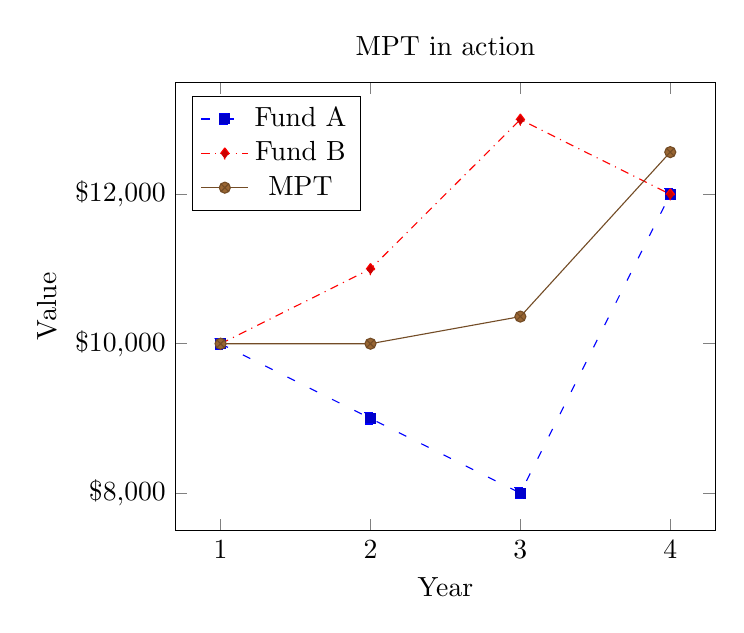
\begin{tikzpicture}
\begin{axis}[
    title=MPT in action,
    xlabel={Year},
    ylabel={Value},
    xtick={1,...,4},
    scaled y ticks=false,
    legend pos=north west,
    yticklabel={$\$\pgfmathprintnumber{\tick}$},
]
\addplot+[
    style={loosely dashed},
    mark={square*},
] coordinates {
    (1, 10000)
    (2, 9000)
    (3, 8000)
    (4, 12000)
};
\addplot+[
    style={dashdotted},
    mark={diamond*},
] coordinates {
    (1, 10000)
    (2, 11000)
    (3, 13000)
    (4, 12000)
};
\addplot+[style={solid}] coordinates {
    (1, 10000)
    (2, 10000)
    (3, 10363)
    (4, 12564)
};
\legend{Fund A,Fund B,MPT}
\end{axis}
\end{tikzpicture}
\end{figure}

At least that's the theory. As usual, reality is more complex. In order for this magical formula to work right, the funds must have a low \emph{correlation} with each other. Correlation is a measure of how similarly a fund tends to behave relative to the others. The two fund examples I used here performed very well and moved in very different ways. While one was going up, the other was going down. This was useful to demonstrate the theory, but it's very hard to find funds that behave in opposite ways like this in reality. They usually move together, and insofar as they do, the magic of MPT is lost.

This is where diversification comes in. It's important to find many funds that are as uncorrelated as possible. The two asset classes that are least correlated are stocks and bonds. Unfortunately, bonds don't perform as well as stocks, so you have no choice but to give up some performance when you use them. Nonetheless, there is no better way to decrease volatility, which is absolutely necessary if your goal is financial independence. I will explain why later.

Another problem in real life is that you can't really predict the correlations. The correlations are volatile too. You can only go on probabilities based on past behaviors. Sometimes everything will move completely in sync, as it did in the October 2008 crash, which was quite brutal for everyone, no matter how diversified they were. Nothing was safe except government bonds, and even those rates soon dropped to 0\%.

Finally, there's some question as to when you should rebalance. In my example, I rebalanced once a year. You should not rebalance more frequently than once a year, but in some cases, it's better to rebalance less frequently. The research that I've found is inconclusive on this.

You can also rebalance more strategically. One technique is to rebalance after a huge, sudden drop or spike in prices. These are the times that you will gain the most advantage from rebalancing. However, such radical changes in the market tend to happen close to each other. You may rebalance after a big drop, only to see it drop significantly more a week later. If you're not careful, this can pull you into becoming a day trader, reacting to the daily whims of the market volatility, rather than the proven strategy of buying and holding.

I conceived a more dynamic approach to rebalancing. This approach only works for ETFs, which I'll explain later. The idea is to rebalance a fund only at the ideal times for that specific fund. Every month, I check the cash portion of my portfolio. If the percentage of cash in my portfolio exceeds my target allocation, then I go into buying mode. If it's less than my target allocation, then I go into selling mode. In buying mode, I look at the funds that are less than their target allocations. I check the 52-week low for each fund, and set a limit order at the price with my broker. Each fund will be rebalanced whenever it drops below its 52-week low and triggers that limit. When I'm in selling mode, I do the same, in reverse. I've found that this strategy performs better historically, incurs fewer costs and taxes, and is safer.

\section{Facing the catastrophe}
When you're investing for financial independence, the goal is to create a portfolio of investments that will dependably provide a steady income. The portfolio you create will be different than it would be if you didn't need it to provide income for several decades, in which case you'd be looking for growth, with little concern for what happens along the way. If your goal is financial independence, then you don't have that luxury. Volatility risk becomes a lot more significant when you're taking money out on a regular basis.

Here's an example of what would happen if you were to take regular withdrawals from an extremely volatile portfolio. Let's say you live on \$30,000 per year, and you have a portfolio worth \$750,000, consisting entirely of 75,000 shares of one stock, which you bought for \$10 per share. The first year, the stock drops drastically, to \$7 per share. You spend \$30,000, which means selling 4,286 shares. Next year, the stock drops again, this time to \$6 per share. You spend \$30,000, which means selling 5,000 shares, leaving you with 65,714 shares. Next year, your investments fully recover, and yet your portfolio is only worth \$657,140. You withdraw \$30,000, leaving you with \$627,140. If your investments had stayed flat this whole time, you'd have \$660,000. This brief but extreme example of volatility cost you 33 grand. And that's after a quick recovery. A protracted recession can be catastrophic in cases of extreme volatility.

\begin{figure}
\centering
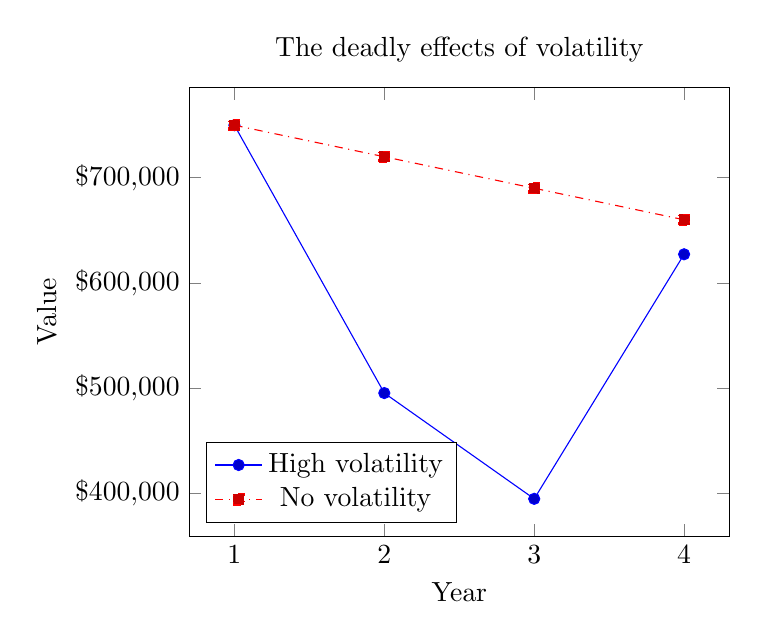
\begin{tikzpicture}
\begin{axis}[
    title=The deadly effects of volatility,
    xlabel={Year},
    ylabel={Value},
    xtick={1,...,4},
    scaled y ticks=false,
    legend pos=south west,
    yticklabel={$\$\pgfmathprintnumber{\tick}$},
    yticklabel style={/pgf/number format/fixed},
]
\addplot+[style={solid}] coordinates {
    (1, 750000)
    (2, 494998)
    (3, 394284)
    (4, 627140)
};
\addplot+[style={dashdotted}] coordinates {
    (1, 750000)
    (2, 720000)
    (3, 690000)
    (4, 660000)
};
\legend{High volatility,No volatility}
\end{axis}
\end{tikzpicture}
\end{figure}

What happened here was that you had to sell more shares in order to reach the same dollar figure of \$30,000. If the stock is selling for \$10 per share, then you only need to sell 3,000 shares to fund your \$30,000 withdrawal, but the year that it dropped to \$6 per share, you were forced to sell 5,000 shares. High volatility has the effect of magnifying your withdrawals.

In this example, the drop happened in the first years of taking withdrawals. It could have also been the reverse, and skyrocketed in the first years, which would have had the opposite effect. If the stock market was booming after you started taking withdrawals, you'd need to spend fewer shares in order to withdraw your \$30,000, thereby increasing your portfolio value. Then, if the same drop happens ten years later, your portfolio would have been much stronger to withstand the same onslaught. So it all depends on timing and volatility.

Volatility risk is one of the greatest investment risks you face when you start taking withdrawals. If you lose a huge portion of your portfolio right off the bat like that, and yet you still need to withdraw money, then your financial future will be in peril.

That's exactly what happened to me.

I retired in February, 2008. The stock market immediately started dropping, and then in October, I faced the greatest stock market crash since The Great Depression. To make matters worse, all of my investments were crashing at the same time, so diversification did nothing to soften the blow. I ended up losing a lot of money. I had some contingency plans, but this was beyond what I could reasonably plan for, so my resolve was really put to the test. All those ``yeah, buts\ldots'' I've heard over the years came to haunt me.

I dropped everything I was doing for six months and focused entirely on the catastrophe. I panicked a few times, then focused, then panicked some more, and focused again. It was scary. First, I looked for even more ways to cut costs that didn't significantly harm my quality of life. Then I pulled out the contingency plans. I had several nice-to-have expenses that I could easily cut in case of emergency. I cut them all, and I was still drowning. I started cutting out some \emph{really}-nice-to-have expenses. Then I started looking for a cheaper place to live.

Meanwhile, I was researching investing again, scouring websites, and reading books. I was trying to figure out how I could have better prevented this disaster and how I can avoid it in the future. Most importantly, I was trying to figure out how to stop the bleeding immediately. Then I did something very naughty: I sold everything.

\emph{Don't try this at home.} If your portfolio is evaporating before your eyes, selling is usually the worst thing you could possibly do. It's the nature of volatility that your investments will recover, and it's the nature of our psychology that our fears will keep us from buying back in before that happens.

However, my choice to sell wasn't out of panic. It was a big risk, and I was perfectly aware of this. It was a decision I made after a lot of thought and research. It was clear that the crash I'd seen so far was only the beginning, but more importantly, I knew this was a unique recession, one never before seen in history. All investment wisdom is based on what we've learned from history. There was no precedent for this. Extreme times called for extreme measures. I may have an investment ``religion,'' but I'm not a fundamentalist. I can still believe in buying and holding index funds, but that doesn't mean that I'm unwilling to make exceptions at the right times, like when I see my entire retirement dream vanishing before my eyes.

The way I figured it, my retirement dream was already gone if I'd let it continue on its present course. Something had to be done. In the worst case, I'd have to go back to work and start over again, and I was already sort of resolved to do this, but at least this way I would go down fighting.

I researched for another few weeks, and then started buying back in, slowly at first, with a whole new portfolio. This new portfolio has several features that I will describe in the next section. I designed it to not only withstand future catastrophes better, but to also take advantage of the current low prices and therefore bring me out even further ahead than when the whole mess started.

The choices I made turned out to be excellent, overall. I was correct that it was only the beginning. It was beneficial to sell when I did and buy back in at lower prices, even though I didn't time it perfectly (no one can). I'd promised myself that I would buy back in \emph{before} it felt safe, so as to avert the risk of not being there for the big recovery. But I did take a huge risk by selling. What if it recovered quickly? I'd have sold at the lowest point, losing a huge opportunity for recovery.

Nonetheless, my plan worked out fabulously. I did indeed end up quite a bit further ahead than when this all started. Only a few years later, I had more money than I had when I first retired, even after inflation. I not only averted the crisis, I used it as an opportunity to position myself even better than when I started.

\section{Investing for growth or income}
As I researched for my new portfolio, I was considering the one disadvantage I had as a retiree: I was taking out regular withdrawals. If this weren't the case, I could have easily weathered the storm and watched everything recover completely. But I knew that even just one or two years of huge losses would be much more severe for me long-term if I took withdrawals in those years.

Like individual stocks, portfolios as a whole also tend to be classified as either \emph{income, growth,} or some combination of both. An income portfolio is one that is designed to give pay-outs at regular intervals, with very little volatility. A growth portfolio is one that is designed to grow over time, with a lot of volatility. This captures the biggest trade-off in investing---risk is usually rewarded with greater growth over time.

I also considered the other unique aspect of my situation: I retired at a young age. That means that I will be holding these investments longer than most retirees, so I have longer to ride out the volatility, even though I will be taking withdrawals along the way. What I needed was a portfolio that was less volatile than pure growth portfolios and more volatile than pure income portfolios, but still provided steady income along the way. What I needed was a combination growth and income portfolio.

As I researched this, one thing that became clear was that I needed more \emph{dividends.} Dividends are regular payments made to shareholders, from the income the companies earn. Dividends do tend to go down during recessions, but not as significantly as the share prices. If I could invest in things that gave more dividends, I figured, and take a larger portion of my withdrawals from those dividends, then I wouldn't need to sell so many shares during recessions. I had avoided dividends before retirement because they are taxed at a higher rate than long-term capital gains, but I'm in a much lower tax bracket now that I'm retired, so avoiding dividends for tax purposes isn't necessary.

Another thing I discovered, or rather, re-discovered, is \emph{costs.} Until then, I hadn't looked as closely at investment costs as I should have. Fees are like the dirty little secret of the mutual fund and brokerage industries. It's in the interest of these industries to avoid talking about them. The only reason they talk about fees to the extent they do is because the Securities Exchange Commission forces them to, and I realized that they still don't tell the half of it.

Despite their low costs, I was running into some limitations of index funds. Like any other mutual funds, index funds are purchased from the mutual fund company itself, each share representing underlying stocks and bonds owned by the fund company. If \emph{you} buy or sell many shares, \emph{they} must buy or sell many shares. This incurs significant costs to the shareholders, so responsible fund companies will institute limits and penalties on how often shareholders may buy and sell their shares.

Another issue with mutual funds, particularly troublesome in volatile times, is that they have up to a one-day delay in their share price, or \emph{NAV.} At the end of each day, they update the NAV, and when you buy, you pay the NAV on the \emph{next} cycle, so you don't know what that NAV will be. That can be risky during times of high volatility.

This was when I discovered \emph{Exchange-Traded Funds,} or \emph{ETFs.} These are a lot like index funds, but they're traded like stocks. You buy them from a stock broker just as you would stocks. There are no limits or penalties on buying or selling shares, since the brokers deal with such large volumes of them, called \emph{creation units.} Since the fund company doesn't have to buy or sell frequently, they tend to be more tax-efficient as well. Since ETFs are handled by stock brokers, rather than the fund companies that offer them, they also have lower trading, management, and marketing costs than even most index funds.

ETFs were initially used by day traders, but their low costs, tax efficiency, and lower volatility risk also made them great candidates for buying and holding. In fact, buying and holding ETFs minimizes their only disadvantage, which is the trading fees. Brokers charge brokerage fees to trade them, just as they do for stocks.

ETFs have their own limitations, however. Due to the brokerage cost of trading them, it's important to find a low-cost brokerage firm. Also, you should only buy ETFs that have a low \emph{average bid/ask spread.} This is the difference between the amount you pay to buy a share and the amount you could sell it for at any given time. It's a hidden cost of trading that must be accounted for. Most ETF companies should be able to tell you the average bid/ask spread of their ETFs.

Something else I did in my new investment strategy was over-invest in stock funds. By the time I bought back in, I had quite a bit more stock exposure than I did before. This caused a bit more volatility during that year as the market struggled to incorporate all the news, but it didn't last very long. First it started to stabilize, then I saw a nice recovery, and a year later, I sold some of them off and bought back into bonds. This allowed me to take advantage of the under-priced stocks.

\section{Buying individual stocks}
Buying and holding a diverse allocation of broad index funds using ETFs is the strategy I use for most of my investing. However, sometimes I use a small portion of my portfolio for more targeted investments. It also serves as a form of diversification, which is what Modern Portfolio Theory requires. Individual stocks and sectors often behave differently than the market as a whole.

When buying individual stocks, the goal is to buy low and sell high. This sounds simple but it's not easy. For one thing, what does ``low'' mean? For most things we buy, we can compare the prices to see which one is cheaper. So it seems intuitive that we could compare the share prices of the investments we want to buy. But a stock price is fairly arbitrary, and depends on how many shares are outstanding.

What you're looking for aren't stocks with a low share price, but stocks with a lower share price than is justified by its value. The same is true for any other kind of bargain-hunting. For example, if you see a car selling for much less than other, similar cars, it might be a bargain---or it might be a lemon. The only way to know the difference is to look under the hood.

There are some ratios you can look at quickly to get a sense for how high or low the price is relative to its assets and its capacity to generate earnings. One such number is the \emph{Price/Earnings ratio,} or \emph{P/E ratio,} which is the stock price divided by the annual earnings, or how much each dollar of annual earnings costs you. This will be lower for investments that have poor future prospects or is not expected to grow much, and higher for investments that are expected to grow. Like any business you buy, you'd pay more for one that is expected to grow quickly.

Another number is the \emph{Price/Book ratio,} which is the stock price divided by the assets owned by the company, or how much each dollar of assets costs you.

Another number is the \emph{Price/Sales ratio,} which is the stock price divided by the annual sales, or how much each dollar of annual sales costs you. Sales are different from earnings. They don't account for the expenses a company has. For example, if a company has a low Price/Sales ratio but a high Price/Earnings ratio, it means that the company is actually really good at earning money, but they're also really good at spending it. Just as you saw in Chapters 1 and 2, both the income and spending components are important. It's often easier to cut costs than it is to get more income, so if you believe the company will do a good job at cutting costs, then this might be a good deal.

After you look at all these numbers, you'll know whether the price is low, but you still won't know why. Just as in the example of shopping for a car: you see the price tag, and you know it's priced low relative to similar cars, but you don't know why. It's up to you as a buyer to closely examine the car and ask the seller questions about it to make sure it's the bargain you hope it is. Likewise, you need to examine an investment, research their balance sheet, income statement, and cash flow statement, read their news, and listen to management conference calls, to determine if it's a bargain. Learning how to do this takes a lot of time, and I'm still a novice myself, but the payoff can be enormous.

Difficult as this may seem, the hardest part of buying low and selling high is actually psychology. Our impulse is to buy high and sell low. When things are going well, we want more of it. When things are going poorly, we want out before it gets worse. It's essential that you be a contrarian. You need to be on a shopping spree when everyone else is talking about the pending apocalypse. You need to be a cynic and start selling off when everyone is talking about how great things are and that it can only get better. This came easy for me because I've always been a bit of a rebel.

When there's a stock market crash, panic ensues. People sell off their investments out of fear. Their fear overpowers their rationality, so they'll sell at any price, even if that price is obviously lower than the company is worth.

During the 2008 crash, some of America's strongest companies were trading at lower than their book value (Price/Book was less than 1). That means that these sellers were saying these companies had no hope of ever turning a profit, that they weren't even worth the property they owned. It was possible that these companies were so worthless that all they could do from now on is lose money, but these were good, solid companies with strong earnings until the big crash. Investors were in such a panic to sell that they were practically giving these companies away. This is an excellent time to snap up some great deals. I bought some shares of a few companies during this time. One of them tripled and another doubled in value in less than a year before I sold it.

\section{Designing your portfolio}
What should your portfolio look like? There are many ways to answer that question. Investing is a personal thing, and depends on many factors specific to you: your age, values, goals, fears, and hopes. I can't tell you exactly what your portfolio should look like, but I can give some general guidelines, and explain the process I used to come up with mine.

I sought out great minds that I trusted. One of these, Warren Buffett, doesn't write very much. However, there were five others that have written good books: Bernard Malkiel, John C. Bogle, William Bernstein, Richard A. Ferri, and Roger Gibson. They each made their own portfolio recommendations, and I used this as a guide. I compared all five recommendations side-by-side and filled in the blanks with educated guesses. I've included two of the five portfolios at the end of this section.

First, decide how you want to divide your portfolio between the two major types of investments: stocks and bonds. This depends on your age and risk tolerance. The more bonds in your portfolio, the less volatile it will be, but also the less it will grow. The younger you are, the longer you have to ride out the storms, so you'll want more stocks because that will give you more growth. If you're older, you'll want more bonds because you don't have the same luxury to ride out the volatility.

Likewise for risk tolerance: if you tend to freak out when there are crashes, you'll want more bonds, but if you know you can keep your cool, you'll want more stocks so you can take advantage of their superior growth. Additionally, once you start taking withdrawals, no matter how old you are, you'll want more bonds because you're much more susceptible to volatility.

Start with an allocation based on your age. If you're under 40, your allocation should be 90\% stocks, 10\% bonds. Starting at age 40, add 3 percentage points of bonds every 2 years. For example, at 40, change your allocation to 87\%/13\%, at 42, change it to 84\%/16\%, etc.

Now adjust for your risk tolerance. If you tend to freak out a little during recessions, add 10 percentage points of bonds. If you tend to freak out a lot, add 10 more. This is your portfolio, so it's entirely your choice how much adjustment you need to make for you to feel comfortable. If you choose something too aggressive for your risk tolerance, and you end up selling out of fear, then that extra little bit of growth you got would do you no good, so if you're not sure, be conservative and lean toward more bonds rather than less.

Once you start taking withdrawals, add another 5 percentage points of bonds, and also consider investing more in dividend-bearing investments.

Next, you must decide how much exposure you'll have to international markets. International investing has historically been important for diversification because they offer relatively low correlations with domestic investments, although that has been changing as our economy becomes more global. Some argue that it's pointless to invest internationally because it's just more risk with little benefit. Others argue that international is the way to go because they believe America will no longer be the economic super power it once was. Most experts believe it's best to have at least some exposure to international investments. How much is up to you. It depends on which experts you agree with and how much you agree with them. I believe 20\% is a good amount of international exposure.

You should now have divided your portfolio into four asset classes. For example, let's say you decided on 60/40 for your stock/bond mix and 80/20 for your domestic/international mix. You just multiply each percentage of stock/bond with a percentage from domestic/international. $60\% \times 80\%$ is 48\% domestic stocks. $60\% \times 20\%$ is 12\% international stocks. $40\% \times 80\%$ is 32\% domestic bonds. $40\% \times 20\%$ is 8\% international bonds.

Now it's time to divide up each of these four asset classes further. For stocks, you have a few different ways you can diversify. One is company size. Large companies perform differently than small companies, so you should have some of both. There are four main size categories: large-cap, mid-cap, small-cap, and micro-cap. Another way to diversify stocks is \emph{growth} versus \emph{value,} which I explained in the Investment Basics section. Both perform roughly the same, but they tend to behave differently, which makes them good candidates for diversification. You should have some of both. You could get them as separate funds, or you could get them both in a \emph{blend fund.}

In international stocks, you have similar distinctions as above, but you can also diversify by region. The main geographical categories are Europe, Pacific Rim, and Emerging Markets. Pacific Rim includes many non-European, first-world countries like Japan, Singapore, and Australia. Emerging Markets includes many of the third world countries. Of the three, Europe is known to behave the most like American stocks and is the least volatile. Emerging Markets behaves the least like American stocks and is the most risky and volatile. Pacific Rim is in the middle, both in correlation and risk. You should probably own some of all three, either separately or together in one fund.

There are non-company stocks you can also buy for additional diversification. A \emph{REIT} is a \emph{Real Estate Investment Trust.} Rather than owning parts of a company, you own parts of corporate real estate. You're paid rent in the form of dividends. You can also buy precious metals and other commodities. Gold is known to be extremely volatile and doesn't perform well long-term, but it may be good to have some in your mix because it tends to have a very low correlation with most other stocks, and is also useful for lowering inflation risk. I don't invest in gold myself.

For bonds, you can diversify based on type, quality, and term. There are government bonds and corporate bonds. Some government bonds worth looking into are \emph{TIPS} and \emph{GNMA.} TIPS is designed to protect you from inflation, which is a good way to lower inflation risk. GNMA is the government mortgage bonds.

The two main categories of quality are \emph{investment grade} and \emph{high yield.} Investment grade bonds are issued by entities with a good credit rating and a history of not defaulting. High yield used to be called \emph{junk bonds} but that name turned people off. High yield bonds are for organizations with poor credit ratings and some history of defaulting, but their rates are much higher to compensate for that risk. So, you can expect the risk and volatility of high yield bonds to be greater than investment-grade bonds, but you can also expect higher long-term growth. For the sake of diversification, it's good to have some of both.

There are short-term, intermediate-term, and long-term bonds. This refers to how long until the loans need to be paid back. The longer the term, the higher the risk, but also the higher the rates. However, long-term bonds don't tend to give enough growth to compensate for its greater risk, so it's better to just stick to short-term and intermediate-term bonds.

International bonds aren't easy to find. As far as I know, there's only one company, DFA, that offers international bond funds that distinguishes between the above three factors, and that company doesn't actually offer these funds to the general public. The amount of international bonds you'll own will probably not be very high anyway, so this doesn't matter much. You can just buy a generic international bond fund. However, there are some good international bond ETFs available to the general public.

How much you divide your portfolio between each of these many types of investments doesn't matter as much as the main two divisions between stocks/bonds and domestic/international. Past this, experts have very different opinions on how portfolios are allocated, but there does tend to be a few common patterns: Growth and value are often divided equally, and it's common to have more large-cap and mid-cap than small-cap and micro-cap, more domestic than international, more Pacific Rim and Europe than Emerging Markets, and more short-term and intermediate-term investment-grade bonds than high yield bonds, TIPS, and GNMA.

\begin{table}[ht]
\caption{Model portfolios}
\label{tab:portfolios}
\centering
\begin{tabular}{l r r r r r r}
\\\hline
\\\hline
& \textbf{Mason} & \textbf{Ferri} & \textbf{Malkiel}\\
\hline
\textbf{\emph{Stocks}} & \textbf{\emph{59.97\%}} & \textbf{\emph{60.00\%}} & \textbf{\emph{65.00\%}}\\
\textbf{U.S. Equity} & \textbf{43.88\%} & \textbf{48.00\%} & \textbf{47.00\%}\\
Large growth & 3.30\% & 15.00\% & 11.50\%\\
Large value & 12.35\% & 15.00\% & 11.50\%\\
Mid-cap growth & 5.63\% & 0.00\% & 0.00\%\\
Small growth & 4.63\% & 0.00\% & 7.00\%\\
Small value & 0.00\% & 9.60\% & 7.00\%\\
Microcap & 2.10\% & 2.40\% & 0.00\%\\
Real estate & 3.80\% & 6.00\% & 10.00\%\\
Speculation & 9.92\% & 0.00\% & 0.00\%\\
\textbf{Intl. Equity} & \textbf{16.09\%} & \textbf{12.00\%} & \textbf{18.00\%}\\
Pacific Rim large & 5.75\% & 3.60\% & 6.00\%\\
Europe large & 1.01\% & 3.60\% & 6.00\%\\
Intl. small cap & 2.81\% & 2.40\% & 0.00\%\\
Intl. value & 1.62\% & 0.00\% & 0.00\%\\
Emerging markets & 4.89\% & 2.40\% & 6.00\%\\
\\
\textbf{\emph{Fixed income}} & \textbf{\emph{40.03\%}} & \textbf{\emph{40.00\%}} & \textbf{\emph{35.00\%}}\\
\textbf{Bonds} & \textbf{34.94\%} & \textbf{38.00\%} & \textbf{30.00\%}\\
Invest. grade & 7.50\% & 7.92\% & 12.50\%\\
High-yield & 4.15\% & 7.92\% & 0.00\%\\
TIPS & 6.97\% & 7.92\% & 5.00\%\\
GNMA & 4.30\% & 0.00\% & 12.50\%\\
Short-term & 8.57\% & 10.29\% & 0.00\%\\
Intl. bonds & 3.34\% & 3.96\% & 0.00\%\\
\textbf{Cash} & \textbf{5.09\%} & \textbf{2.00\%} & \textbf{5.00\%}\\
Money market & 5.09\% & 2.00\% & 5.00\%\\
\hline
\end{tabular}
\end{table}

As an example, Table~\ref{tab:portfolios} at the end of the chapter shows my current portfolio target allocation next to two of the five model portfolios I based it on, from the books \emph{All About Asset Allocation} and \emph{A Random Walk Down Wall Street.} These books didn't spell it out exactly like it is on this table, but I filled in some of the blanks myself in order to compare them side-by-side.

Due to the differences of opinion between the experts, and individual factors such as age, goals, and risk aversion, this is really something you need to customize. I made many choices that disagreed with the experts because I weighed the arguments made in the various books and decided where I stood on those, and whether they applied to me. I favor value and mid-cap companies; I want lots of dividends; I add a small speculative element; and I don't want to invest in oil or gas. Then I tweaked the numbers based on my age, goal, and risk tolerance. I also occasionally tweak this target allocation as things change or as I incorporate new information.

Not only is creating an asset allocation the most personal part of investing, it's also the most important to get right. Most investing experts agree that your asset allocation has far more impact on the performance and risk of your investments than which funds you choose. So, don't spend all your time shopping for funds. Spend more time refining your asset allocation. There are many good books on this subject, some of which are included in the Resources.

\section{Taxes}
Many people are painfully aware of how much payroll taxes they pay, so it's ironic that so few account for it in their investments. This is probably because investment taxes are relatively invisible compared to payroll taxes. They don't show up on their paychecks or monthly statements. But like every recurring, incidental expense, taxes can have a huge impact over time. They are just as important as fees. In a sense, they \emph{are} fees, just paid to a different organization.

Taxes are very political. The major division between each political philosophy is on how this money is collected and spent. Pretty much everyone disagrees with at least one thing the government spends money on, and they don't want to support that with their income. On the other hand, we all use the services the government provides. Some resent it, while others are grateful for those services and are glad to support them.

Taxes should be fair, and it's up to our elected officials to create a fair tax system. They will offer credits, deductions, and adjustments to incentivize certain things and allow for exceptions to the basic tax rules. Your job as an investor is to learn about which of these are relevant for you and take advantage of them. In other words, your goal is to minimize the taxes you're required to pay. This is an easy sell for those who resent taxes, but even if you want to support the system with your taxes, you should still take advantage of all the tax incentives offered to you because that's an important part of the system.

The most fundamental aspect of our tax system is that it is based on earning and spending money. Income tax is for the money you earn, and sales tax and property tax is for the money you spend. Financial independence involves minimizing the amount of money you spend in order to minimize the money you earn. Therefore, by the very nature of the tax system, the closer you get to financial independence, the less you'll be required to pay in taxes. You'll be spending less, so you'll be paying less sales tax. Your food and drug costs will be a larger portion of your total spending, which are not taxed at all. You'll also be earning less, so you'll pay less in income taxes, at a lower tax bracket. More of your income will come from long-term investments, which is taxed at a lower rate than salary.

Interest and dividends are taxed at your normal tax rate. There are also \emph{capital gains,} which are the gains you get from selling an investment at a higher price than you paid for it. The IRS distinguishes between two holding periods. \emph{Short-term capital gains} are gains you made on investments that you held for one year or less. These are also taxed at your normal tax rate. However, \emph{long-term capital gains}, for investments you held for more than one year, are taxed at much lower rates. If your tax bracket is 25\% or higher, you only pay 15\% for your long-term capital gains, which is nearly half of what you'd normally pay. If your tax bracket is 10\% or 15\%, you pay zero taxes on your long-term capital gains.

It's possible to keep your income so low that you pay zero taxes on your long-term capital gains. Take a look at your current tax schedule to see what income this means for you. You will also want to minimize your short-term capital gains. That means only selling your investments if you've held them for at least a year. If you re-balance your portfolio no more frequently than one year and one day, then this should be taken care of for you.

You should also minimize interest and dividends, since these are taxed at your normal rates. This is especially important while you're earning a lot and saving for financial independence, since you'll be in a higher tax bracket. There are a few ways to minimize dividends. One is to invest inside of a tax shelter, which I will talk about shortly. Another way is to use \emph{tax-managed funds.} Another way is to focus on growth funds more than value funds. Once you go into a lower tax bracket, however, it's not quite as important to minimize dividends. I have found that the added advantage of a more stable income outweighs the need to minimize dividends for tax purposes once I achieved financial independence and started taking regular withdrawals.

You should also minimize the \emph{turnover} in any funds outside of tax shelters. Turnover is the percentage of the holdings in a fund that are bought and sold each year. You're not only taxed on the capital gains that you get from buying and selling the fund as a whole, but also from the buying and selling that happens \emph{within the fund} throughout the year. These taxes can really add up fast for high-turnover funds. Look for funds with less than 50\% annual turnover. Index funds are, by their nature, extremely low-turnover funds. Avoid high-turnover funds or put them in a tax shelter.

\emph{Tax shelters} protect your investments from taxes, mainly for retirement purposes. One tax shelter is the 401(k) and 403(b) retirement plans (named after the section of the tax code that created them). You get these through an employer. They deduct a certain amount from your paychecks. Many of them also \emph{match} your contributions, which means that they will pay some amount to your retirement plan for each amount that you pay. You will not be taxed on this or its growth until you retire. I recommend that you take advantage of this matching feature as much as you can, up to the limit. Once you leave your job, you may \emph{roll over} (which is just a fancy way of saying ``moving'') your money from your 401(k) or 403(b) plans into an IRA or Roth IRA.

An \emph{Individual Retirement Account,} also called an \emph{IRA} or \emph{traditional IRA,} does not depend on your job. IRAs provide the same benefits as an employer-sponsored plan with more flexibility but lower contribution limits. Unlike an employer-sponsored plan, you can invest your IRA in anything you want---stocks, bonds, savings accounts, CDs, etc. The IRA itself is just a tax mechanism. Whichever investment vehicle you choose, the IRA only means that you don't have to pay taxes on what you contribute or on its growth until you withdraw it.

For the 401(k), 403(b), and IRA, you will be taxed when you take withdrawals. This is called \emph{tax deferral.} This is very much to your advantage because your earnings will have grown tax-free for all those years, and you will probably be in a lower tax bracket when you start taking withdrawals.

A \emph{Roth IRA} is very similar to an IRA, but is the opposite from traditional IRAs in one significant way. In an IRA, you're not taxed on what goes in, but on what comes out. In a Roth IRA, you're taxed on what goes in, but not on what comes out.

Whether you would be better off contributing to an IRA or Roth IRA depends on your tax bracket. If you're in a high tax bracket, you'd be better off contributing to an IRA because you won't be taxed until you're in a lower tax bracket later. You can also later convert an IRA to a Roth IRA and get taxed right away if you go into a lower tax bracket.

However, Roth IRAs are better than IRAs for most people. It's usually better to pay taxes right away and not pay any taxes on its growth, because over time, the growth of investments tends to far overshadow the original contributions. Another advantage of the Roth IRA is that you can withdraw the original contributions any time you want,\footnote{The one exception is that you must wait 5 years before doing so for any money you've converted from a traditional IRA to a Roth IRA.} so the Roth IRA can also serve as a supplemental emergency fund.

Another tax shelter is a \emph{Health Savings Account} or \emph{HSA.} There are health insurance plans that incorporate these. You put money into this account tax-free, which can grow over time. When you get sick, you can withdraw the money tax-free. This is an excellent option for people who are relatively healthy, due to their extremely low monthly premiums and tax savings.

There are also tax shelters for saving for education, but most tax shelters are designed for retirement.

The government has a very specific idea of what retirement means. On the surface, their definitions may seem to differ from those who want financial independence in the form of early retirement. The standard rule is that you can't retire until you're $59 \frac{1}{2}$ years old. However, they provide a little known exception to this rule for early retirees: you may withdraw your money from your IRA or Roth IRA at regular intervals, on a schedule according to your life expectancy. This is called the \emph{72(t) exception.} All the IRS cares about is that you're actually retired, and not just taking money out whenever you feel like it. Therefore, once you start taking withdrawals on a schedule, you must continue doing so indefinitely.

You might not even need to use 72(t). If you're investing a lot of money very quickly, you will hit your tax shelter contribution limits, so you will also be investing money outside of your tax shelter. Once you start taking withdrawals, start with money outside of your tax shelter, and once you've depleted that, then start taking regular withdrawals from your IRA or Roth IRA. Once you've started taking withdrawals from a Roth IRA, you will be able to withdraw all your original contributions tax-free, and will only need to use the 72(t) schedule once you've depleted that.

I actually pay \emph{zero taxes,} legally and with no loopholes. First, I invested heavily in my 401(k), paying zero taxes going in. Once I became financially independent, I rolled over everything into an IRA. After the crash, when I sold everything and bought a whole new portfolio, I reported huge losses that will take me years to recapture. This way, I have zero income for tax purposes, except for the year I sell my home. I would have negative income, if that were possible.

Between this negative income and deductions, I have some wiggle room to move money from my IRA to Roth IRA each year, tax free. Once it's all in my Roth IRA, I can withdraw all of my money tax-free. My expenses are so low that my income will be in the 10\% or 15\% tax bracket, which means that all long-term capital gains from anything not in the IRA or Roth IRA will also be tax-free.

Homeownership also has its perks. Many of the biggest costs for homeowners are deductible from taxes. Mortgage interest and property taxes are entirely tax deductible. Plus, any gains you get from selling it for more than you bought it are also tax-free (up to a limit). You get even more benefit if you rent out some rooms in your home, because this allows you to deduct a portion of your maintenence and repair expenses as well.

In summary, the best way to minimize the tax you're required to pay is to earn and spend as little as possible, use tax shelters, own and live in a rental home, use tax-managed funds outside of your tax shelters, and keep high dividend and high turnover funds in your tax shelters. Maximize your contributions to your 401(k) or 403(b) first, then maximize your contributions to your IRA or Roth IRA, and then invest normally. IRA is tax-free going in and taxed coming out, while Roth IRA is taxed going in and tax-free coming out. It's better to use a Roth IRA unless you're in a higher tax bracket. It's possible to pay zero taxes if you keep your income low enough and you slowly convert your IRA to a Roth IRA over time, with enough deductions or capital losses to capture those conversions.

\newpage
\section{Resources}
\begin{itemize}
\item \textbf{\emph{A Random Walk Down Wall Street,} by Burton Malkiel.} This is the best investing book I've read. I consider it essential reading. It explains everything you need to know about investing, in the most down-to-earth fashion I've ever seen, but without dumbing it down. It demonstrates the Random Walk theory of investing. It is a little long-winded, but it's worth it.

\item \textbf{\emph{Common Sense on Mutual Funds} by John C. Bogle.} If you can only read one investing book, read \emph{A Random Walk,} but if you can read two, read \emph{Common Sense.} When you read this book, you'll understand just how vital it is to minimize investment costs. Although this book is a little dry at times, the way Bogle exposes the evils of the mutual fund industry is amazing.

\item \textbf{\emph{All About Asset Allocation} by Richard A. Ferri.} If you can only read two investing books, read \emph{A Random Walk} and \emph{Common Sense,} but if you can read three, read \emph{All About Asset Allocation.} Other books explain how investing works, but fall short when it comes to the nuts-and-bolts of putting together an actual portfolio. This book assumes you know how investing works, and just explains how asset allocation works and how to put together a good portfolio.

\item \textbf{\emph{Value Investing For Dummies} by Peter J. Sander and Janet Haley.} Don't let the title fool you. Although it's very accessible for the layman, it's also very thorough and detailed. I've read several books on value investing, and this is the best. If you want to learn how to determine if a stock is worth the price, this book will teach you.

\item \textbf{\url{https://advisors.vanguard.com/}} -- The website for Vanguard financial advisors.

\item \textbf{\url{https://personal.vanguard.com/us/funds/tools/recommendation}} -- Vanguard's balanced fund recommendation engine. Answer a few questions, such as risk tolerance and time horizon, and it will recommend a balanced fund intended to meet your needs.
\end{itemize}

\chapter{Open For Business}
\fancyhead[CO]{\emph{Open For Business}}
\fancyhead[CE]{Freedom Beckons}

\section{Balance sheet and cash flow}
One of the clich\'es in personal finance is that you should treat your life like a business. I used to figure this was a kind of business worship, as if business isn't just something you do to put food on the table, but a lifestyle, even a spiritual practice.

But in some ways, our lives are very similar to businesses. We have different motives, of course. Rather than a profit motive, we have a love motive, a joy motive, a safety motive, and a comfort motive. But like businesses, we trade our services for money. We have money coming into and out of our lives like a business does, and we have some amount of investments and cash on hand like a business does. But since businesses are so laser-focused on the profit motive, they have developed some very effective tools for managing those things, which we can use in our own lives.

One tool is called the \emph{balance sheet.} This is simply a list of everything you own, called \emph{assets,} and everything you owe, called \emph{liabilities.} Subtract the liabilities from the assets to come up with the balance. This represents your \emph{net worth.} You should also calculate your \emph{liquid net worth,} which you will need for your withdrawal rate calculation. This is simply your net worth minus any assets you can't or don't intend to sell in order to raise cash.

Another useful tool is the \emph{cash flow.} This is an outline of all the money coming into and going out of your life.\footnote{The cash flow as I describe it here is not quite how a business does it, but it's the same basic idea.} The first part of your cash flow is your job income. The second part is your investment income. The third part is your expenses. You will need to know your expenses for your withdrawal rate calculation.

In order to keep track of your cash flow, you will need to keep records of everything you earn and spend. Every penny. Some people find this intimidating, but I found it easy once I got used to it. I just keep receipts, and later I record the expenses. Sometimes, I'll depend on my memory, and write it down when I get the chance, but it's so easy to forget to write them down later. It's also possible to use credit card statements or bank statements, but these aren't as detailed, so it's harder to pay close attention to your trade-offs.

You can look into personal finance software that will make the balance sheet and cash flow easier for you. Another option is spreadsheet software. That requires you to organize it all and construct the formulas yourself, but it does allow for the most flexibility. If you hate technology and have plenty of time on your hands, you can also do it by hand with a pen, paper, and a calculator. I use a spreadsheet to maintain my records.

In its simplest form, a balance sheet looks something like Table~\ref{tab:balance-sheet}

\begin{table}[ht]
\caption{Balance sheet}
\label{tab:balance-sheet}
\centering
\begin{tabular}{l r}
\\\hline
\\\hline
\textbf{Assets} & \textbf{\$162,000.00}\\
\hline
Cash & \$500.00\\
Checking account & \$1,500.00\\
Savings account & \$5,000.00\\
Balanced fund & \$50,000.00\\
Roth IRA -- Balance fund & \$100,000.00\\
Car & \$5,000.00\\
\\
\textbf{Liabilities} & {\color{red} \textbf{-\$500.00}}\\
\hline
Credit card & {\color{red} \$\-500.00}\\
\\
\textbf{Total net worth} & \textbf{\$161,500.00}\\
\textbf{Liquid net worth} & \textbf{\$156,500.00}\\
\end{tabular}
\end{table}

This can become more complex if you have lots of investments or loans. You only need two columns: the name and the amount. You have an assets section and a liabilities section. List everything you own and everything you owe, of any significant value. At the bottom, there are two calculations. The first is your total net worth. Simply subtract your total liabilities from your total assets. Then calculate your liquid net worth. In this example, I deducted the value of the car from the net worth to get the liquid net worth.

\begin{table}[ht]
\caption{Cash flow}
\label{tab:cash-flow}
\centering
\begin{tabular}{l r l}
\\\hline
\\\hline
\textbf{Income} & \textbf{\$3,000.00}\\
\hline
09/01/2015 & \$3,000.00 & Net salary\\
\\
\textbf{Interest} & \textbf{\$910.00}\\
\hline
09/05/2015 & \$10.00 & Savings account\\
09/30/2015 & \$300.00 & Balanced fund appreciation\\
09/30/2015 & \$600.00 & IRA appreciation\\
\\
\textbf{Expenses} & \textbf{{\color{red} \-\$1,084.49}}\\
\hline
09/01/2015 & {\color{red} \-\$600.00} & September rent\\
{\color{blue} 09/02/2015} & {\color{red} \-\$1.99} & {\color{blue} Soda}\\
{\color{blue} 09/03/2015} & {\color{red} \-\$25.00} & {\color{blue} Dinner with friends}\\
09/04/2015 & {\color{red} \-\$150.00} & DVD player\\
09/05/2015 & {\color{red} \-\$300.00} & Clothes\\
09/30/2015 & {\color{red} \-\$7.50} & Brokerage fee\\
\hline
\end{tabular}
\end{table}

Table~\ref{tab:cash-flow} shows an example of cash flow for one month. There are three sections. In the income section, list all of your paychecks and tips. This section is only relevant while you have a job. The second section is your investment income. List the interest you earn in your accounts, the growth or losses of your investments, and the dividends you receive. The third section is your expenses, the most important of the three. List here all the money you spend. This example only shows a few days of expenses, but you'll have an entire month of expenses in this section. 

The first column is the date of the transaction. The second column is the total amount of the transaction. The third column is the name of the transaction. Due to limited space, I could not show all possible columns, but there are some other columns you may wish to add.

You might find it useful to create a column for the category of the transaction. If you have detailed records for your expenses, you may want to get a summary grouped by categories such as rent, transportation, food, etc. It's up to you how you categorize your expenses. For example, some people like to have two categories for transportation: one for their automobile, and one for everything else.

I also find it indispensible to have a few columns to represent \emph{amortization.} This is a fancy word, but all it means is that you distribute the amount of a transaction over its entire lifetime. Most things you buy aren't monthly expenses. Without amortization, they will disappear from future month expense statements, even though you're still getting value from it. For example, one of my utility bills comes every other month. I could put the entire bill on one month's spreadsheet, and then nothing the next, but the more accurate way to do it is to put half this month and half next month. You could choose to amortize only your big costs, but I do it for every transaction with a lifetime of two months or more.

When I first started maintaining my cash flow, I didn't use amortization, and it wreaked havoc on my planning. One month, my costs would be extremely low, and I'd pat myself on the back. The next month, my costs would shoot through the roof, due to a large expense. It was impossible for me to calculate my withdrawal rate with any hope of accuracy.

To do this, I've added three extra columns, which I did not show in the table due to limited space. One is the \emph{amortized value.} This is the total cost divided by its lifetime. For example, if the utility bill that comes every other month was for \$100, the amortized value is \$50. This column is calculated automatically from the other two columns I've added, representing the lifetime. One column is the date of the expense and the other is the end of the lifetime. For the bi-monthly utility bill, I would put today's date in one column and next month in the other column. For some expenses, this is only an estimate, but I find that even an inaccurate amortization is better than no amortization at all.

There are some hidden expenses you should remember to include in your Expenses section. One is brokerage and investment fees, because the withdrawal rate calculations don't account for these. Brokerage fees are more obvious because you have to actually pay them when you do your trading. Mutual fund fees are a lot more hidden. Mutual fund companies will deduct management fees from your fund each year unless you agree to send them a check or give them some other source of payment. Management fees in ETFs are even more hidden because they're actually deducted from the share price. It's not very clear when the deductions take place, or for how much. What I do is divide the expense ratio by 12 months, and multiply that by the ETF balance in my Expenses each month.

Another hidden expense you need to be aware of is car depreciation, if you own one. Cars lose a significant amount of value over time, and this really is an expense. You spend money just by owning and driving the car.

I use colors in the spreadsheet as a mnemonic. You can get as creative with this as you like. Whatever makes your spreadsheet easier for you to read and understand. My spreadsheet shows the negative values as red. I also use blue for every row that isn't a recurring transaction. Every transaction that is amortized will not be highlighted, but I also don't highlight recurring, monthly transactions, such as utility payments. When I make the next month's spreadsheet, I simply copy all of the black rows from the previous month, and update the date, until it expires.

These spreadsheets are for your own records only. Spreadsheets are very flexible tools. Put anything there that you think will help you reach your goal. As you get more practice with them, you may think of even more uses for them, and you'll become more efficient when you update them.

\section{Regular updates}
Many businesses update their public records quarterly (every three months). You could do it every week, every year, or anything in between. I do mine every month, so that's what I'll use in my examples. If you do update your balance sheet and cash flow infrequently, it will require less work and you'll see less volatility in your investments, but you'll also be working with outdated information much of the time. More frequency wins you better information upon which to base your trade-offs.

I keep track of every transaction I make. I keep a record of all the money that comes into or goes out of my life. I've found that you can be as specific as you want. For example, when you go grocery shopping, you could just record the whole trip as ``Food'' or you may record every transaction separately. Being more specific takes more work, but provides you with very detailed records, which I personally find extremely useful. The first spreadsheet I did, in 2003, was very sparse and simple compared to my modern spreadsheets. So if you want to start with the easier, less detailed record keeping, it's fine if you decide to change it later.

Most spreadsheets allow you to create multiple sheets in one document. I use this feature to keep all spreadsheets related to the balance sheet in one document, and all spreadsheets related to the cash flow for the same year in one annual cash flow document. Each month, you can make a copy of last month's sheet, and then work with that, so you have monthly records of your trends, or you can simply overwrite last month's sheet each month. I find it very helpful to have records of prior months' cash flows, and not so helpful to keep prior month's balance sheets.

The first thing I do each month is balance my checkbook. I look at my bank records, check off everything in my checkbook that coincides, and correct any inconsistencies. This ensures I always have an accurate checkbook.

Next, I update my balance sheet. I count all of the cash I have on hand, and look at my bank records, brokerage statements, and credit card statements (most banks make these available online as well), and update my balance sheet to reflect them. This gives me a new net worth and liquid net worth. I keep records of the monthly values, and I construct a graph that shows these trends over time.

In my balance sheet document, I also maintain a spreadsheet for my asset allocation. This shows the percentages of each asset compared to their target allocations, which will get skewed over time. Whenever I re-balance my portfolio, I use this as a guide for how much I need to buy and sell of each asset.

Next, I update my cash flow. When I was working, I would look at my paycheck each month to update my job income section. Then I look at my bank statements, brokerage statements, and credit card statements, and list any interest I pay or earn in my investment income section. I also list the growth of my investments, by comparing this month's value with last month's. Since I do not re-invest my dividends, I also include here any dividends my investments earned.

Finally, I finish updating my expenses for the month. When I'm done, I have a grand total of job income, investment income, and expenses. I construct a graph for the trends here as well. The big pay-off came after years of working with these spreadsheets and I could see the trends of my job income, investment income, and net worth trending upward as my expenses drop.

\section{Paying yourself first}
``Paying yourself first'' is a common phrase among financial planners. What it means is that your first priority should be your future: you should deduct from your income all the payments for saving for retirement, and then use whatever is left over to pay your bills and other incidentals.

Many people use their income as a gauge for how much they have to spend each month. There is a psychological tendency to spend what we earn, whatever that is. As earnings increase, so does our appetite for spending. Paying yourself first short-circuits this tendency, so that the only earnings you see, and therefore believe is available for spending, has already accounted for what you need to reach your goals.

However, I've always thought there was a big problem with this philosophy: most of what people spend \emph{is} for themselves, unless they are philanthropists. Whether they buy food, pay their utilities, or buy something that brings them joy, that money is for themselves, so spending this money \emph{is} paying themselves first. Just because they're giving their money to someone else doesn't mean they're paying someone else before themselves.

The above technique that financial planners recommend assumes that you can \emph{afford} to pay off your debt and invest for retirement. When I started on my goal, I was nearly starving. At one point, I had enough money to either buy oil for my motorcycle or food for my belly, and I chose my belly. I still had to get to work, so I drove my motorcycle without oil and destroyed the engine. This wasn't stupidity. It was desperation. Choosing to eat rather than paying off debts was what ``paying myself first'' looked like for me.

The problem with the strategy of investing for your future first is that it treats this as the top priority, and it obviously isn't. You shouldn't deny this in order to play some sort of psychological trick on yourself. As I mentioned in Chapter 2, you should make your choices consciously, so you can make the right trade-offs at all times. If you do this, then you don't need to trick yourself into investing for your future. You will always know which choice is the most important to you, whether it be for your current needs or future goals.

What, then, should be your priorities? Here is a summary of the entire process of achieving financial independence, in order of priority.

Your first priority, obviously, should be your survival and the survival of your loved ones. Once your basic needs are met, then you must decide what's most important for you. You may have some desires that are more important to you than freedom. Start with that first. That's what paying yourself looks like for you.

Once you have your basic survival needs met, and a few desires that bring you immense joy that is worth more to you than your freedom, only then is it time to start thinking about financial independence. That would be a good time to create the balance sheet and cash flow spreadsheets so you can keep track of your progress toward this goal.

The first part of this you should focus on is increasing your income and advancing in your career, the subject of Chapter 1. You need money to achieve financial independence, and your job is your source of money, so you need to think about how you can make more money. Make a plan for your income growth.

Next, you need to drop your expenses, the subject of Chapter 2. I say this is the second step, but you can start on it right away. Also, unlike your income, there is no glass ceiling, and unlike investing, you're not done once you've decided on a strategy. The process of dropping your expenses is on-going. Keeping expenses low is the backbone of financial independence.

After you've made a plan to increase your income, and you started working on dropping your expenses, you should start noticing some nice trends in your balance sheet and cash flow. Your net worth should be going up, your income should be going up, and your expenses should be dropping. Once you start spending less than you earn, you will need a place to put all that extra cash, the subject of Chapter 3.

If you have debt, this will probably be the most logical place to start. I recommend consolidating your debt as much as possible, and then just chug through it. It can help to create an amortization schedule for your loan payments. There are online tools to help you do this. I've included one in the Resources. It will show you how much interest and principal you are paying with each payment, and how many such payments you will need to make to pay off your loan. This can help put your debts into perspective.

Pay your debts off before you start investing, except for loans with really low rates. Start paying off debts with the highest rates first. Think of your loans as high-interest, risk-free savings accounts. You'd want to invest in the highest interest account first. Once you're left with only low-rate loans (less than, say, 5\%), you might be better off just paying the minimum payment and investing the rest.

Before you start creating a portfolio of stocks and bonds, prepare for emergencies and unforeseen circumstances like losing your job. You should have a certain amount in a savings account for such circumstances. Some people feel fine with only a month or two worth of living expenses. I recommend at least two months. I chose six months. It felt really good that I could be out of work for a half a year and still make ends meet. Once you do your cashflow spreadsheet, you should know your monthly expenses. Just multiply that number by however many months you choose.

Now you're ready to start constructing your portfolio. This is where you really need Chapter 3. You should start by taking advantage of every tax shelter available to you, up to the limits imposed by the government. Probably the best place to start is with a 401(k) or 403(b), if your employer offers one. 401(k) is not only the most important tax shelter---it's also the easiest. It's deducted directly from your paycheck pre-tax, so you don't need to make any changes on your tax return. Your tax payments are automatically adjusted accordingly, so the impact is huge while the effect on your bottom line is not as noticeable.

Once you've contributed to your 401(k) to the maximum allowed by law, then invest in an IRA or Roth IRA, as I mentioned in Chapter 3. The limits for these are much lower than the 401(k). Contribute to an IRA or Roth IRA to the maximum allowed by law.

Once you've maxed out your 401(k) and IRA or Roth IRA, you can start investing your money outside of a tax shelter. If you do this, look into tax-managed funds, as I mentioned in Chapter 3.

\newpage
\section{Resources}
\begin{itemize}
\item \textbf{\url{http://www.edmunds.com/used-cars/}} -- Gives you the true market value of a used car, which you can use to estimate depreciation.
\item \textbf{\url{http://www.amortization-calc.com/}} -- An online calculator for creating an amortization schedule for your loans.
\end{itemize}

\chapter{Meet Your New Boss}

\section{Retirement}
So far, I've focused primarily on financial independence, and rarely mentioned retirement. Retirement is a choice that is only available to those who are financially independent, so it's relevant, even if you choose to work till the day you die. When people think of retirement, many imagine a life of lethargy. There's a clich\'e image of a golf course in Florida, or a hammock on the beach. Some people picture a retirement home. Why would anyone want to retire, if that's what they have to look forward to? I don't play golf, and I don't like the beach very much. I prefer my retirement to reflect my own passions, not some stereotype.

As I explained in the Introduction, I define retirement as \emph{permanently severing the connection between labor and income.} This is my own definition, for the purposes of this book. It's the only definition that draws a distinction from unemployment, sabbatical, or changing careers, and has no age restrictions.

Financial independence offers choices. It's not an all-or-nothing proposition. You could work only part time. You could take a lower paying, but more enjoyable job. You could volunteer. You could take a sabbatical. You could go back to school and take your time exploring a new career. You could consult occasionally, or take a seasonal job for fun an some extra cash. You could quit any time you want, and go to the beach or play golf or ride a motorcycle or travel or go for a hike on a beautiful day or read books or spend time with friends and family. You're only limited by your own imagination.

I've seen the word \emph{semi-retirement} used to describe this partial form of retirement. Your retirement is yours to do with as you please, and you're free to call it whatever you like. Retirement is a state of mind. It helps some people to think of themselves as retired, even if they still accept money for their labor. 

For me, full retirement is the logical conclusion of financial independence. Selling my time feels too much like selling myself, setting aside my own values and passions and temporarily taking on someone else's. During that time, employers all too often feel entitled to treat me however they like. The knowledge that no one else has a lease on my life, not even one minute of it, affords me the kind of freedom I've craved since childhood. When I retired, I stopped holding back, and fully embraced life, because I knew it was all mine.

\section{Whim and Will}
Many people use their jobs as a self-discipline crutch. They know people are counting on them, and they know there will be dire financial consequences if they slack off. Even when they really don't want to work, they force themselves to do it anyway. They become so accustomed to this pressure that they fear what would happen to them if they retired, and suddenly found themselves without the structure and discipline of working full-time. After decades of this kind of life, many retirees feel lost, and go back to work out of sheer boredom. Structuring your own time and looking within yourself for motivation are important skills retirees must have.

There are many analogues between employment and retirement. For example, I still feel like I have a boss. His name is Whim. Whim expects me to work days, nights, and weekends. I'm always on-call. The pay is lousy, but the benefits are great. I work from home every day, my hours are totally flexible, and I set my own deadlines. Best of all, I love my job. My job is to follow my passions and curiosities, wherever they lead. It's an important job, and I take it very seriously.

Whim is the most demanding boss I've ever had. He reminds me every day that the stakes are very high: life or death. Do I want to live my life, or am I just waiting to die? When I worked full-time, it was easy to neglect the things that mattered most to me. Some things I had to put off until Saturday or Sunday, but most things I put off for an eighth day that never came: Someday.

Now that I'm retired, every day is Someday. It's now or never. I can't get away with putting things off, because, if not now, when? This forced me to be much more serious about the trade-offs I make in life. I no longer live under the delusion that Someday will come and give me plenty of time to live my life. This now-or-never attitude led me to learn more about self-discipline.

I was always lousy at self-discipline. I define it as \emph{the ability to force yourself to do something you don't want to do.} I've always believed self-discipline makes people mechanical. I figured, if I really don't want to do something, then why would I do it? It's my life. And if I really want something, then why would I need to force myself? Wouldn't I just do it? Self-discipline is entirely unnecessary, and could actually mean I'm spending time doing things I don't \emph{really} want to do. So I vowed to only do things I want to do, and devoted my life to Whim.

Many motivational speakers teach that self-discipline is like a muscle. The more you use it, the more you have. They say things like, ``resolve today to\ldots'' or ``make a commitment to\ldots'' As if it's just a matter of deciding to do something. If it were that easy, there would be very few smokers, and Alcoholics Anonymous wouldn't exist.

Forcing yourself to do something you don't want to do requires a tremendous amount of willpower. Willpower is not a muscle. Each person has a limited supply, which becomes even more limited when they're stressed or tired. This is why, for example, judges give harsher sentences for trials they rule on later in the day. They lack the willpower they had in the morning to be as careful and meticulous about weighing the evidence. It's also why people tend to be exhausted after working all day, and just want to do something easy. Working full-time takes tremendous willpower. They've used up all their willpower working for someone else, and then they have very little left over for themselves.

Achieving financial independence requires willpower. This can be a catch-22: you have to work, which depletes your willpower, which you need to achieve financial independence, so you don't have to work. You'll have to learn to conserve your willpower as possible. The following is what helped me do this.

It takes a lot more willpower to do something you don't want to do than something you do. As much as possible, avoid self-discipline. If you use the word ``should'' to describe your attitude about something, you're probably using self-discipline. When you really don't want to do something, you'll procrastinate more. This requires a lot of willpower, just to not think about the thing you ``should'' be doing. By the time you get around to it, often close to the deadline, your willpower will be drained, you'll be miserable, and you'll probably do a lousy job on it.

The highly successful people that motivational speakers love to praise for being ``disciplined'' don't actually use a lot of self-discipline. Instead, they're highly motivated, which is self-help jargon that obscures its true meaning: \emph{they really want what they want.} They aren't forcing themselves to do things they don't want to do because they want to do what they do, very badly.

Think about what you do want, not what you don't. The mind tends to create what it thinks about. This is called the \emph{self-fulfilling prophecy.} New Age spiritualists call it the \emph{law of attraction,} but there's nothing esoteric about it. It's just a natural capacity of the mind. If you think about what you don't want, you may unconsciously work to bring it about. It's a lot more effective and motivating to focus on what you do want.

It takes more willpower to do something after you've just finished doing something that takes less willpower. We naturally have a kind of inertia. When we're at rest, we like to stay at rest, and when we're busy, it's easier to stay busy. Imagine trying to clean your house after coming home from a party. It's a lot easier to clean the house and then go to the party. Try to arrange your day so that you get the hard stuff out of the way before you relax and have fun. When you do have fun, just have fun. Don't worry about everything you need to do, because worrying takes willpower.

It takes more willpower to do something new than something old. The bigger the change, the more willpower it takes. Human beings are creatures of habit, but this varies from person to person. Some people thrive on new things, and can change habits quickly. These are the few people who can quit destructive habits ``cold turkey.'' Some habits can only be changed suddenly, which makes them more resistant to change. Fortunately, most habits can be changed slowly. When done in this way, it should feel fairly painless.

I've found there are three stages I go through whenever I start a new habit, or quit an old one. The first is the \emph{honeymoon stage.} It's brand new, and the brain loves novelty. I'm excited about the results I might see from the change. It takes less willpower in this stage, because I'm highly motivated. The second is \emph{boredom.} The novelty has worn off, and it becomes a bland routine. Since change takes a long time, I become discouraged because I'm not seeing results. This is the stage that requires most of the willpower, and is when I'm most likely to give up. The third is \emph{habituation.} This is when I've become so used to it that it's the new normal. It still takes some willpower, but it may actually require more willpower to quit.

One important habit you'll need for financial independence is \emph{thinking long-term.} This is a bit different than a behavioral habit. It's habit of thought, which requires mindfulness. You have to watch your mind, and notice its cravings. You have to think about your conflicting desires, short-term vs. long-term, and ask yourself what you \emph{really} want. Your mind might say, ``chocolate donut.'' Your old habit is to just head to the pantry and stuff a donut in your mouth. Instead, you have to think about what you want long-term. If what you \emph{really} want is to be healthy, then you'll skip the donut. You must be honest about what you really want. If you \emph{really} want to be healthy, then the donut won't seem so interesting by comparison. But if you really want the donut, you'll find a way to get it, whenever you're low on willpower.

This long-term thinking is often associated with self-discipline, when it's usually called \emph{delayed gratification.} This isn't self-discipline as I've defined it, because it's not forcing yourself to do something you don't want to do. You're only making a conscious trade-off between two conflicting wants, and you choose the greater of the two wants. Long-term goals like financial independence take time to grow and come to fruition. Anything that involves slow growth requires planting seeds, and waiting. Fortunately, the delayed gratification is only temporary. Consider this: if you plant one seed a day, then you'll have to delay gratification every day only until your first harvest. Once you harvest your first plant, then you can harvest another one every day thereafter, as long as you continue planting one seed a day. You don't really have to delay gratification indefinitely. You just need to pay that upfront cost, and then you can go right back to instant gratification. That's good news, since it takes a lot of willpower to delay gratification indefinitely.

It's not a moral failing to prefer a short-term want over a long-term want. Sometimes there's nothing better than a delicious chocolate donut. Besides, the whole point is to live a happy and fulfilling life. How is it possible to have a fulfilling life without chocolate? What matters is that you make your choices with your eyes open. Understand the trade-offs, and choose wisely. Be honest with yourself. Much is at stake.

Ultimately, all wants are short-term wants. Every choice you make can only be made at the moment it arises. That's short-term. You have to decide what is most important to you right now. That's why I say Whim is my boss. He's in charge of what I really want in life. He guides how I use my willpower. Whim can work together with willpower. They make a great team.

\section{Withdrawal rate}
Whim pays me a very small salary, and is pretty stingy about raises. The compensation package I get is called the \emph{withdrawal rate.} This is something I've alluded to a few times already, but I'll go into more detail now. The withdrawal rate is the amount of money you spend each year, divided by your liquid net worth.

\begin{center}
Withdrawal rate = Annual expenses $\div$ Liquid net worth
\end{center}

If your liquid net worth is zero or less, then your withdrawal rate is undefined.

In Chapter 4, you learned how to develop spreadsheets to calculate your monthly expenses and liquid net worth. Now you have everything you need to calculate your withdrawal rate, which is the most important number for your quest toward financial independence. This number will serve as a gauge of your progress toward this goal.

Using the example in Chapter 4, let's say you add up all your expenses, and you find that you spend \$2,500 a month. Then you add up all of your liquid assets and subtract any money you owe, and you find that your liquid net worth is \$156,500. Your withdrawal rate would be:

\begin{center}
Withdrawal rate = \$2,500/month $\times$ 12 months $\div$ \$156,500 = 19.16\%
\end{center}

Your goal for financial independence is to decrease this withdrawal rate over time. You do this by saving more money (income, Chapter 1, and investing, Chapter 3) and spending less (frugality, Chapter 2). For example, suppose you cut your costs by \$100/month, and you've stashed away \$2,000 in your investments:

\begin{center}
Withdrawal rate = \$2,400/month $\times$ 12 months $\div$ \$158,500 = 18.17\%
\end{center}

You will have achieved financial independence when you've dropped your withdrawal rate down to or below your target withdrawal rate. Your target withdrawal rate depends on several factors, so you will need to calculate it yourself. I've included in the Resources section the best online withdrawal rate calculator I've found.

No one has just one target withdrawal rate, but a range of safety. What a withdrawal rate calculator does is back-tests a certain investment strategy to give you some range of withdrawal rates and how likely they have been in the past to ensure that your money survives. In other words, in some past stock and bond market scenarios, at any given withdrawal rate, you'd have spent too much money, and ran out before your life expectancy. Running out of money is the death blow for financial independence, especially if you've been out of the workforce for a long time. The calculators can't tell you what the future holds, but it can give you some range of probabilities, based on past behavior, what you can reasonably expect your odds to be. You have to decide for yourself what kind of odds you're comfortable with. The higher the odds of success you choose, the more money you'll have to save, so the longer it will take. It's up to you.

A very common target withdrawal rate, which leans toward the overly conservative side, is 4\%. This is the target withdrawal rate that I personally use, and will use here. 4\% is a very safe withdrawal rate. I usually keep my withdrawal rate even lower than that. My reason for this is the idealism I mentioned: I refuse to go back to work. Ever. I preferred working a little longer so I could guarantee that when I'm done, I'm really done. 4\% is also very convenient because it's a nice round number, so it's very common. Please substitute your own target withdrawal rate when you see me use 4\%. That includes the 25 rule and the 300 rule. If your target withdrawal rate is 4.5\%, for example, then you'd use a 22 rule ($1 \div 0.045$) and a 267 rule ($12 \div 0.045$).

I think it's useful to create a spreadsheet for this in your balance sheet file. Create a row for your liquid net worth, and a row for your monthly expenses. Then make a row for your current withdrawal rate, which is 12 times your monthly expenses divided by your liquid net worth. Then make a row for your target withdrawal rate. Once your withdrawal rate drops below your target, then you have achieved financial independence! Meanwhile, this number will probably be very large, maybe even in the hundreds or thousands. If you're in debt or have no savings whatsoever, this number is essentially infinite. That's fine! As you make progress, this number will drop.

You can watch the trends of your dropping withdrawal rate, and maybe even construct a graph for this. I must warn you, however, that these trends are not linear, due to how ratios work (the math term for this is \emph{asymptotic}). The progress you make early on will have much greater impacts on your withdrawal rate than the same amount of progress will have as you start approaching your target withdrawal rate. This can be exciting at first, as you watch your huge leaps of progress, but as you get close to your goal, it can be frustrating, as you watch your withdrawal rate crawling closer to your goal, somewhere below 10\%. Those last few percentage points are the hardest. Just keep this in mind and know that, as long as this number is dropping, you are making progress.

Your target withdrawal rate is only a guess about what the future holds. I probably don't need to tell you that the future usually turns out a lot different than we expect. We can plan the best we can, and use reasonable guesses to facilitate that, but you should remember that you're only guessing. You have to be ready to adjust your plans as things change.

The withdrawal rate probabilities are most heavily affected by what happens in the first two years of withdrawing money. These are big growth years that set the stage for the rest of your lifetime of withdrawals. If you get a lot of growth in these first years, then you'll end up with more money than the withdrawal rate estimated. If you lose money in these first years, you'll be more likely to end up with just enough or not enough money than the withdrawal rate predicted.

Plan the best you can. Pad your expenses. Keep a low withdrawal rate. But don't be paranoid. At some point, you need to trust that you've planned the best you could. If you don't, you risk becoming a miser. Remember, the point of this is to have a life of freedom and joy, not paranoid slavery to your own fears and insecurities.

\section{Your new paycheck}
One common feature of jobs that people think goes away with retirement is the almighty paycheck. Not so. Retired people get paychecks just like everyone else, although they may look a little different. In retirement, ``paychecks'' are called ``withdrawals.''

Once you start taking withdrawals, your ``income'' is simply your target withdrawal rate multiplied by your liquid net worth. For example, if your withdrawal rate is 4\%, and your liquid net worth is \$750,000, then your annual income is \$30,000/year ($4\% \times \$750,000$).

You should have a cash account of some kind to take withdrawals from throughout the year. This could be your checking account, savings account, money market fund, or laddered CDs. Laddering CDs means that you have one Certificate of Deposit for each month. One CD would mature each month, which gets deposited into your checking account. So, you'd have a 1-month CD, a 2-month CD, a 3-month CD, a 4-month CD, etc., up to a 12-month CD. Each year, you'd open up 12 more, or you could just open a new 12-month CD every month. The idea is that since you know you won't need that money until the maturity date, you can take advantage of the higher rates CDs theoretically offer.

However, I've found that CDs don't offer very high rates. I've always been able to find a savings account that offers a higher rate than even a 1 year CD. So, why bother with all the complexity of laddered CDs when I can get a higher rate in a simple savings account? But do your own research and do what makes sense for you.

If you choose to use a savings account, what you could do is put 1 year of living expenses in a savings account, or maybe a little less, since you'll be earning interest on it throughout the year. Each month, you could make deposits into your checking account from your savings account, and that would be your paycheck. Each year or so, you should re-balance your portfolio. You will be selling some of your assets and buying others. That's the time to replenish your savings account or CDs.

Don't worry if you run out of cash before the year is up. It's fine to sell assets that have appreciated higher than your target allocation. You should also have a good amount of short-term, investment-grade bonds in your portfolio, which are much less volatile than other investments. They aren't quite as safe and stable as a savings account, but it doesn't hurt to pull from it occasionally when you need the cash.

\section{Getting raises}
It's impossible to know ahead of time exactly what your withdrawal rate should have been. The best you can do is look at past trends and estimate a target that would have kept you relatively safe in those scenarios. But the future \emph{will} be different than those scenarios, which means that your withdrawal rate \emph{will be wrong.} The idea is to choose a conservative enough withdrawal rate that the future will be even brighter than the scenarios you've planned for, and you will end up with even more money than you expected. In other words, your boss gives you a raise!

The traditional withdrawal method is to simply take your liquid net worth on the day you start withdrawing from it, and withdraw only 4\% of \emph{that} each year. No matter what your investments do or what your withdrawal rate becomes, you keep your spending even. This works fine except for periods of high volatility and high inflation.

After you've been taking withdrawals, you may find that your liquid net worth grows over time, and your withdrawal rate is dropping. Some of this is to be expected, since the stock market can be very volatile, so your money may shrink again, causing a spike in your withdrawal rate that restores it to its target, or goes over the target for a while. But if your liquid net worth continues to grow and your withdrawal rate keeps dropping, at some point it's good to assume that your target withdrawal rate was too low, and you're free to spend some more. In other words, you get a big raise after many years of conservative spending. I don't use this method for that reason. I'd rather get lots of smaller raises along the way rather all at once down the road.

On the other hand, if you notice your liquid net worth shrinking, and your withdrawal rate climbing, after a while that could be a sign that the initial withdrawal rate you chose was too high. This is dangerous, because at some point, you'll run out of money. There are only two ways to fix this: spend less or earn more. It will be much harder after several years of over-spending. That's another reason I don't use this method. I'd rather make smaller adjustments as they prove necessary, using a buffer to protect against volatility putting me in a constant state of feast or famine.

The other methods are more dynamic, and involve tracking your expenses to your withdrawal rate. This is difficult because, between surprise expenses and market volatility, your withdrawal rates will jump around like a pogo stick. How can you know what is safe to withdrawal if your withdrawal rate won't stay still? There are a few approaches.

One is to have a buffer. Whenever your withdrawal rate drops below 4\%, set aside a portion of your ``raise.'' Whenever the withdrawal rate jumps over 4\%, use up the money you set aside in previous months to bring it back to 4\%.

Another method, suggested in the book \emph{Work Less, Live More,} is called the ``95\% rule.'' Whenever your withdrawal rate goes over 4\%, drop your expenses as much as 95\% of what you spent last year. The author found that it's fairly safe to spend that much, even during bear markets.

The method I use is to pick a range of acceptable withdrawal rates, and simply ignore the volatility within that range. I usually keep withdrawal rate below 4\%, so I don't worry about it if my withdrawal rate occasionally gets as high as 4.5\%. 5\% is my panic button. That's when it's time to make significant changes. This is pretty conservative, as even 5\% can be a somewhat safe withdrawal rate for diversified investments.

One monkey wrench in your planning is inflation. I've talked about inflation risks in Chapter 3, but I didn't explain how it will effect your planning. \emph{Your Money or Your Life} suggests you simply ignore inflation risk entirely, which would be convenient since it would simplify your planning. However, in this book, I don't suggest you ignore this risk, which means you need to plan for it.

Inflation is the drop in value of your money over time. In five years, you will be able to buy less with the same money that you have now. If you didn't have investments that outpace inflation, then it would be to your advantage to spend that money as quickly as possible, rather than investing it for the future. So, if you're trying to figure out how much money you'll have and how much you'll need at some point in the future, which is necessary for financial independence planning, you'll need to account for inflation.

The problem is, inflation is hard to predict, and therefore hard to plan for. Some Chicken Little economists warn of stagflation or hyperinflation since our economy no longer depends on a gold standard. Others say the dangers of inflation is exaggerated. It's up to you whose opinion you trust the most. All I recommend is that you not ignore inflation risk entirely, and that you try to plan for it the best you can.

All withdrawal rate calculators take inflation into account, and I believe most of them use the \emph{Consumer Price Index,} or \emph{CPI,} to measure it. That's why the withdrawal rates they give tend to be low versus the growth you can expect from your investments. If you use the traditional method, then once you start taking withdrawals, you need to increase the amount you are allowed to take each year to account for inflation. So, this is another way your ``boss'' gives you a raise. You can assume this to be 3\% per year, which is a conservative estimate of inflation. In the example I gave earlier of a liquid net worth of \$750,000 and an annual income of \$30,000, your raise in the first year would be \$900, bringing your income up to \$30,900. The second year, it will be \$927, bringing your income up to \$31,827. And so on.

There is another form of inflation that is often ignored, which I call \emph{age inflation.} As we age, in addition to prices, our own expenses also change. In most cases, they drop. We've already accumulated a lot of the things we want, we've finished paying off our mortgages, the kids have moved out and gone through college, and we can move to a smaller home in a less expensive area. You may want to plan for these changes. But there is one way that we can expect our expenses to go up as we age, and that is in our health care.

\section{Health insurance}
\emph{Health care} is deceptively named. It's actually illness care. Aside from annual exams, most people don't actually use it unless they get sick. Health care has more to do with your lifestyle than with your doctor. Caring for your health is mostly up to you, by how you eat, sleep, work, and how you spend your time. The best way to save on illness care costs is to decrease your need for it, which mostly has to do with how you live, although genetics and environment are also factors.

\emph{Health insurance} is also deceptively named. Most health insurance is actually health maintenance contracts. Insurance covers you in rare cases of financial hardship. So, true health insurance wouldn't actually come into play unless you become seriously ill or injured. Such plans do exist, and they have extremely low premiums. Look for health insurance with high deductibles and low premiums, and then do what you can to stay healthy so you won't need it. HSAs, which I mentioned briefly in Chapter 3, come with such insurance.

It's difficult to predict what will happen with health care in the future. Health care costs are out of control. Liberals argue for government-sponsored health care for all, while conservatives think the government has its hands in too much of the economy as it is. All that is clear is that health care costs are ridiculous, the rate at which it's going up is not sustainable, and at the time of this writing, there is still no complete solution.

If you are getting health insurance from your employer, then that is a hidden part of your total employment compensation package. This is income that will go away when you leave your job, so it's income that you will need to make sure you provide for yourself. I recommend that you talk to an insurance broker and estimate how much you'll need to pay for health care once you're financially independent, and include that cost in your expenses for your withdrawal rate calculation.

There is a legally mandated health insurance called \emph{COBRA,} which is really just your former employers' health insurance that you pay for instead of your former employer. COBRA is extremely expensive. Most individual health insurance is much cheaper. However, there is a law called \emph{HIPAA,} which says that insurance carriers can't hike up their rates on you as long as you meet certain conditions, and one of those conditions is that you have continuous coverage. Another condition is that you must use COBRA until it expires, so that would be a reason to use COBRA.

In addition to planning for health insurance in your projected expenses for the purpose of your withdrawal rate, I also recommend that you set aside a certain portion of your net worth for a rise in health care costs and emergencies over your lifetime. I call this \emph{health insurance insurance.} Don't include this portion in the net worth for the calculation of your withdrawal rate. Treat it as money you can't use for funding your financial independence. How much you set aside is up to you. You could guess, or you could talk with an insurance broker and make some projections. When I did this, I decided to plan for my premiums to go up 35\% every five years, in addition to the standard inflation rate. Just make sure that when your health care costs go up, or emergencies come up, you deduct the principal specified by your withdrawal rate for these costs from the portion you set aside for this purpose.

Since health insurance is so completely broken and even corrupt in some ways, you face the risk that your health insurance provider will refuse to pay your claims for bizarre reasons, and their well-paid lawyers will make sure they can get away with it. Additionally, if you do get seriously ill, you will suddenly start paying the full deductible each month, which will cause your expenses to go up. This isn't just a problem with health care, but any catastrophe that comes up that insurance doesn't cover. And it isn't just a problem for people who aren't working. Having a paycheck each month doesn't mean that that paycheck will be enough to pay for any catastrophes that come up. You must set aside money for that.

Insurance doesn't cover you for every possible risk. You should have an extra cushion in your savings that you set aside for emergencies. Either don't include this in your withdrawal rate calculations, or change your target withdrawal rate to account for it. Some people may think it's better to just get lower deductible insurance, but if you think about it, that's actually the same thing except that you're giving that extra money to an insurance company for one specific purpose, rather than keeping it for yourself, to use for any purpose. Consider how much higher your monthly premium would be if you got insurance with a lower deductible. Multiply that by 300, and that is the extra cushion you need to set aside. You could either dedicate that to paying your insurance company, or you could keep it for yourself.

It's impossible to predict and plan for every contingency, but health care is one of the likeliest culprits of raining on your financial independence parade, if you don't plan for it well enough. Once you're old enough to qualify for Medicare, your health insurance costs will drop again. However, Medicare is limited, so you should still plan to have health insurance, which is called Medi-gap insurance.

\newpage
\section{Resources}
\begin{itemize}
\item \textbf{\url{http://www.passionsaving.com/retirement-calculator.html}} -- This is the best withdrawal rate calculator I've found.

\item \textbf{\url{http://www.ehealthinsurance.com/}} -- This is an online health insurance broker that is very easy to use and compare providers. 
\end{itemize}

\chapter{Yeah, But\ldots}
\fancyhead[CO]{\emph{Yeah, But\ldots}}
\fancyhead[CE]{Freedom Beckons}

\section{Excuses}
``Yeah, but\ldots'' are words I often hear when I tell people about financial independence. When I hear these words, I take it as a sign that they don't really want financial independence so much as to convince me or themselves that my situation is unique, or their situation is unique, so they can't achieve financial independence. If you're focused on the reasons you're unable to do something, then you'll be unable to do it.

I'm not here to tell you how to live your life, or what choices you should or shouldn't be making. To do so would completely miss the point of what I'm trying to do. My goal is to help you increase your amount of freedom, and freedom means making your own choices. All I want to do is present new perspectives to help you re-evaluate your choices. If you're totally happy with your choices, and confident that they are right for you, then you don't need this book.

These are all of the common ``yeah, buts'' I've heard over the years, along with my rebuttals. Some of them are about financial independence, and some are about early retirement specifically. If you're not interested in financial independence, these rebuttals are not intended to change your mind. But if you are serious about it and you have some doubts, or you're having trouble with people in your life having doubts, refer to these.

Of course, it's up to you to find solutions to your own problems, and the first step in doing that is to believe with all your heart that you will. My answer to your concerns may sound insufficient or discouraging, but it doesn't mean you should give up. It only means there's no easy answer that I know of, so you'll need to use your determination and creativity to find your own answer.

\section{Yeah, but\ldots I don't earn enough money}
It's a common myth that you need to have a ton of money, and therefore need to earn a ton of money, in order to achieve financial independence.

You do need a lot of money, but probably less than you think (see Chapter 5 to help you figure out exactly how much you'll need to earn). Financial independence is also a factor of how much you spend and how you invest your savings, which is under everyone's control, no matter how much they earn. Financial independence is the inevitable result of living beneath your means, and spending less than you earn. If you can do this, then you can become financially independent.

The only real questions are, how long will it take, and is it worth it for you? If you don't earn very much money, that means you will have drop your expenses even more, and it will take you longer. It may not be worth all that effort for you to be financially independent, but that's a different issue.

Additionally, it's also possible to earn more money. You could change careers or advance in your existing career. Think about your skills and your gifts, and look for creative ways to put them to better use to earn you more money. This is the subject of Chapter 1.

\section{Yeah, but\ldots I have so much debt}
People who have a lot of debt feel very weighed down by it, so it seems impossible for them to ever get out of the hole. The compound interest of debt has the effect of pulling people down further and further, even as they pay it down as fast as they can. It's like running a race in which you start far behind the starting line, with a head wind against you. You run as hard as you can, and you wonder if you'll ever make it to the starting line, let alone the finish line. This is why debt can feel very discouraging, but it's not hopeless.

We all start somewhere. You have only one place you're capable of starting: right where you are. You can blame yourself for getting into debt, and you can wish you didn't have to start so far behind the starting line, but when it comes down to it, blaming and wishing won't \emph{change} where you are. You must start where you're at, for better or worse. The only way to change where you are is to start by accepting where you are. The only way to get out of debt is to pay it off. Wishing you didn't have to pay it off won't pay it off any sooner.

I too started out with some debt. One way I found to make it more encouraging was to treat it like investing. When I accepted where I was, I treated my interest payments as something like rent, just inevitable payments I must make to maintain my life. This way, any extra I pay is like an investment, which earns interest, by taking away from the payments that I'd otherwise have to make in order to maintain my life. The interest rate of this ``investment'' is equal to that of the loan I'm paying. For example, when I had a car loan at 8\% interest, I figured, what a great deal! Where else would I find a savings account that would earn me 8\%, risk-free? I excitedly invested in this savings account called my car loan.

Some people have a lot of debt. When you look at your amortization schedule (which I mentioned in Chapter 4), you may feel overwhelmed. You may find that it will take you many years to pay off your debt, so you may wonder why you should even bother. But those years will pass whether you pay off the debt or not. You can either stay in debt in those years, or you can get out of debt. Choosing to stay in debt doesn't make the debt go away. It only means you'll have to pay it later, after paying even more interest on it.

It is possible to achieve financial independence if you're in debt. It only means that it will take longer. Debt doesn't disqualify you from financial independence any more than a low-paying job or high-cost commitments. Even with debt, a low-paying job, and high-cost commitments, it is possible to achieve financial independence if you want it badly enough---if you work especially hard at the steps I outline in this book. Your biggest limit is your own devotion to your goal.

Even if you make your amortization schedule and you estimate that you won't be able to achieve financial independence for a long time, even if you do the steps in this book, that still doesn't mean that you can't achieve financial independence. It only means that it will take you longer than you would like. But your only other choice is to not do the steps in this book, in which case it will take you even longer. I know it's discouraging to have such a lousy choice, but no matter how long it will take you, doing the steps in this book will always allow you to achieve financial independence sooner than you would have otherwise, and the time you get back is your own precious life.

\section{Yeah, but\ldots I have to support a family}
Freedom is even more important for families than for single people. A lot of parents get so wrapped up in supporting the family financially that they miss the whole point. Do you spend as much time with your family as you or they would like? Would you like to learn to be a better parent, but can't find the time to read books or attend workshops? Many families are well-off, even wealthy, but they suffer from a severe time poverty. They make the wrong trade-offs. That's what financial independence is all about: finding the right trade-offs.

As a head of household, your expenses will be higher than they'd be if you were single, but the problem is not fundamentally different. You need to question all of your choices just as you would if you were single. What is it that truly brings you and your family joy? Is it lots of stuff, or is it plenty of quality time with people you love? Even if you don't retire early, the program in this book will give you more time, more options, and less stress. You may choose to cut back your hours, or change to a job or career that isn't so demanding, allowing you to spend more time with your family.

One advantage you have with a family you live with is that you can share a lot of costs. If you're single, you need to buy one of everything for yourself, in smaller portions. With a family, you have an economy of scale. You can share many of the things you buy, and you can buy more things in bulk. Make sure you leverage that advantage as much as possible. Besides, isn't sharing what love is all about?

For lots of tips for how to save money while strengthening your family, take a look at \emph{The Tightwad Gazette,} listed in the Resources. Amy Dacyczyn was so good at frugality that she was able to live in a large farmhouse with plenty of land and raise a very large, happy family, while spending less than most single people do. She did work she loved, which afforded her a lot of time with her kids, and then retired early. You may not choose to be as frugal as her, but it's good to know what's possible.

\section{Yeah, but\ldots isn't it better to find work you love?}
A common misnomer is that there is a compromise between finding work you enjoy and achieving financial independence. Who said you have to choose? Why not find work you love until you become financially independent?

When you're forced to work for a living, your livelihood is at the whim of supply-and-demand, which can be pretty merciless. Everyone wants to do what they love, but there are only so many lovable jobs to go around, so most people end up doing work they don't much care for. Loving their job is something everyone seems to believe is possible, but few actually pull off.

So, yes, definitely look for work you love. Don't let financial independence get in the way of your search. If you do find a job you love, then count yourself lucky. If you don't find work you love, also remember that it is not a personal failure. So many career books make it sound like everyone can find a job they love, which leads people to wonder what's wrong with them if they can't. Nothing is wrong with you. It's simply a negative side effect of supply-and-demand. Work at the best job you can find, with the right trade-offs, and enjoy it as much as you can. Once you become financially independent, you'll have a lot more control over your life.

A good tip in general when working toward financial independence is to maintain an \emph{``and'' attitude} rather than an \emph{``or'' attitude.} Look for ways you can get everything you want in life \emph{and} become financially independent. Don't create artificial trade-offs. If you think you've found a trade-off, a choice between a higher-paying job you hate and a lower-paying job you love, keep searching for a higher-paying job you love. Don't just give up.

If you keep searching and you really can't find it, then, yes, you must choose what is more important to you. This is a difficult trade-off that only you can make. That still doesn't mean you have to choose between finding work you love and financial independence. It only means that it will take you longer to achieve financial independence than it would at the worse job.

\section{Yeah, but\ldots I like my job!}
This was the strangest thing. All my life, I'd hear people grumble about their jobs, and ``thank god it's Friday.'' I'd hear songs with titles like ``Take This Job and Shove It.'' I'd see coffee mugs with a bedraggled worker on Monday morning. I'd hear about various techniques used by workers to manage the drudgery of their time at work, like ``clock watching'' and ``looking busy.'' Then when I suggested that it's possible to escape this, suddenly everyone starts loving their jobs.

Maybe some of them do like their jobs, but just need to grumble occasionally about some of its less savory aspects. It's got some downsides, but on balance, they get more benefit from working than not working. But then I wonder, if they do in fact like their jobs so much, why don't they do more of it? It seems unlikely they would want to do the exact amount of work that is contractually required of them. You'd think, if they get the most benefit from their lives when they're at work, then the best thing they can do is to work as much as possible. Few people do this, and when they do, they're called workaholics.

I think what's happening here, at least in part, is good old fashioned rationalizing. For one reason or another, financial independence, and the steps required to achieve it, doesn't appeal to them. They don't like working, but they also don't want to do what's necessary to stop. And that's totally fine, but I wish they would just say that.

However, I suspect they haven't really thought it through. In fact, before they met me, I doubt most of them have even considered the possibility. People don't like being caught off-guard like this. They don't like to appear ignorant or complacent. The easiest way out of this cognitive dissonance is a quick rationalization. They figure there are actually parts of their jobs they like, so then they act like they've fully considered the possibility of financial independence and rejected it because they like their jobs.

I'm just speculating here. I don't really know what's going on in their heads. It could be that everyone I talked to before I wanted to achieve financial independence hated their jobs, and then suddenly I just started meeting tons of people who love their jobs. This is probably at least partly true, since I shifted from blue collar work to white collar work right around this time, and white collar work tends to be less humiliating and provides more autonomy. Still, I suspect there's a fair bit of rationalizing going on as well.

Even if you like your job, financial independence can make it even better. Financial independence gives you more flexibility and safety. You can get a better education to improve your job even more. You can weather lay-offs much better. And things change---you may burn out some day. You might decide you'd rather do something else. You'll know you're at your job for the right reasons. You're there because it enriches your life, not just your wallet.

Unless you plan to die at your workplace, you will have to retire some day anyway. Why not choose for yourself when that will be, and do some planning? If you plan to retire at 65, why is that? Is that really when you want to retire, or are you just going along with the default? If you really like your job, why would you ever want to retire?

All I'm saying is, be honest with yourself. Ask yourself some hard questions about the choices you're making in life. If you ask yourself these questions, and you're happy with the answers, then that's great. This book is for those who are still asking.

\section{Yeah, but\ldots what's wrong with working for a living?}
There's nothing wrong with working. I love working, when I choose it. What I don't want to do is \emph{work for a living,} to depend on that job for my livelihood.

It depends on your motivation. Are you working because you want to, or because you \emph{have} to? If you're not financially independent, then you \emph{have} to, whether or not you \emph{want} to as well. If you cherish freedom, I would think this would bother you.

Here's a weird analogy. Let's say you want to play a game of golf with your buddies. Then I put a gun to your head and say, ``play golf with your buddies, or die.'' Does that change anything for you? If you care about your freedom, I expect it would. It doesn't matter how much you'd want to do it anyway---this coercion will inevitably change that golf game for you. It would certainly make it much harder to enjoy the game. It also calls into question whether you actually wanted to play it in the first place. It gets really hard to be honest about your motivations as a free agent when you're no longer a free agent.

I'm talking about freedom, not work. It's possible to work and be free, and it's possible to not work and not be free. If you choose to work, then work. But if you wouldn't choose to work if you didn't have to, or you wouldn't choose the specific kind of work you're doing now, then you're not free. If your livelihood is tied to your work, then your authentic motivations will always be distorted by your motivations for survival, so it's difficult to be sure about what you \emph{really} want.

\section{Yeah, but\ldots what about \emph{right now}?}
One misunderstanding I heard when I told people about my goal of financial independence is that I am making huge sacrifices right now for some glorious future. What if I die before I retire? Won't I wish I lived it up now? What about all the things I'm giving up for this goal?

Every choice you make should be one of getting more out of life, not less. Not every choice needs to be getting the maximum joy out of life this very second. If it were, then there would be no reason to go to school or college. We make investments in our future all the time. The real issue they seem to have, then, is that the investment I'm making is above and beyond what's \emph{culturally acceptable,} ignoring what's \emph{personally acceptable} for me.

The way I see it, I spent 8 years in college so I could have a better life afterward, and then I spent another 8 years in work so I could have a better life afterward. Why are the second 8 years so different from the first? It's not that I had to suffer and sacrifice during those 8 years in college, or the 8 in work. I enjoyed learning and contributing as much as I could, given my lack of freedom. I spent my free time doing exactly what I wanted to do, and I wasn't afraid to spend money if I knew it would bring me great joy.

Something the objectors didn't see was how much better my life \emph{already was} than only a few years before, and this improvement was directly attributable to the choices I'd made to manage my money better and work toward financial independence. These choices didn't just benefit me toward my goal of retiring early---they had immediate benefits.

This goal didn't introduce any new sacrifices or trade-offs for me. All it did was make me \emph{conscious} of my trade-offs, so I could make wiser trade-offs. Maybe people saw this as some great sacrifice because I was making different choices than they personally believed are necessary for happiness. I craved freedom, not jet skis and sports cars. My tastes simplified as a result of this goal, and therefore what made me happy had shifted from what made most other people happy.

\section{Yeah, but\ldots there are other forms of freedom}
Indeed, there are many forms of freedom, and although I focus on it, this book isn't only about financial freedom. I will describe some other freedoms in the next chapter.

When I hear this ``yeah but\ldots'' usually they'll offer some examples of freedoms they cherish or crave. The most common ones I've heard are: the freedom to not worry about money and the freedom to travel a lot or live an expensive lifestyle.

What's happening here is that two different concepts are being conflated. What they are talking about are actually forms of \emph{abundance.} What I'm advocating for is \emph{liberty.} While I agree that it can feel very freeing to travel a lot or to not worry about money, these aren't basic freedoms in the same way as the ability to make your own choices in life without coercion.

There's a good analogy for this, called the \emph{gilded cage.} Suppose you lived in a beautiful, golden cage, only allowed out occasionally and briefly. Would you feel free just because you may enjoy the beautiful sight of precious metal? Perhaps you would, and if you had the choice between living in such a cage and not living in a cage at all, you would happily choose the cage. If that's true, that's fine, but I believe many people feel differently.

Those who say this ``yeah, but\ldots'' tend to be middle- or upper-class and have jobs that afford them a lot of autonomy, at least enough to meet their needs, and therefore they don't feel much like they're living in a cage at all. All I can do is wish them the best of luck with a lifestyle they clearly prefer.

When I began my quest for financial independence, this was not the way I was living. When, largely thanks to this quest, I did earn enough to become middle-class, I was granted more freedom. But by this time, it didn't feel like I was freed---I was just given a bigger cage, and I was just as determined to escape. I believe there are others who also feel this way, and that's who this book is for.

As for the freedom to not worry about money, I believe this simply doesn't exist for anyone. To be human means putting some thought into how you are going to meet your needs in life which, in a capitalist economy, means finding ways to sufficiently accumulate and spend money. Whenever you learn a trade, go grocery shopping, or interview for a job, you are doing this, even if indirectly.

Most people, no matter how wealthy, would say they would love to earn more money than they presently do, which illustrates how insatiable our appetites for wealth can be. Most people feel that pinch, that wish to do more than their current means allow. This is why credit cards are so popular. Financial independence doesn't create this pinch, and earning more money doesn't make it go away. It may alleviate it somewhat, but it also might make it worse, since our wants tend to grow as our means grow.

The popular way to alleviate that pinch is to have more of what you want, but there's a second way, which most people overlook: \emph{you can learn to want what you have.} I can absolutely say I feel that pinch less than ever before in my life. This is true for both reasons: I've increased my means and have been able to afford more of what I want, but I've also learned to be more content with a simple life.

I also have an issue with the word, ``worry.'' To worry about something is to be extremely concerned about and preoccupied with it, and I just don't feel that describes my relationship with money after I started on my financial independence goal. In fact, I worried about money constantly before this goal because I was always running out of it. I was worried every time I went to the ATM, wondering whether this would be the time it finally denies me cash. My financial independence goal freed me from this worry entirely. I always knew exactly where my money was, and I always had plenty of it.

I do make \emph{plans} regarding money, sometimes intricate plans, a process I quite enjoy. I became very conscious of my money and my spending, so I would never have to worry about it. I don't think being aware of something and being careful about the trade-offs I make with it constitute ``worrying.''

I only think about money when I'm doing something with it. The same is true for working. If you're making careful plans about a particular project while you're at work, and then when you go home, you forget about it, that's just planning. But if you feel preoccupied with it all the time and extremely concerned about the outcome, then your planning has turned into worrying.

Financial independence doesn't mean worrying about money all the time, but it does require thinking about money in new ways. If you have no interest in doing this, that's fine, but rejecting financial independence because you think it will require worrying about money whereas without it you never would, this is likely untrue.

\section{Yeah, but\ldots won't you get bored?}
You know what I find strange is that no one ever thought to ask me that until I started working full-time. As a child, I had summers off. No one expected I would be bored if I didn't have a job. I did get bored sometimes, but that tended to be when I got tired of playing with one thing and was looking for the next fun thing to play with. What I really found boring was school.

Now that I'm retired, boredom looks a lot more like it did when I was a child. I become bored when I tire of one thing and I'm looking for something else. Boredom is a sign that my flame is dying and it's time to re-ignite it.

When boredom comes, I try not to rush to fill the void. I find boredom and lethargy to be productive downtime. It's a time when I'm most open for inspiration. I'm ready to take a new path when it opens up for me. I might spend weeks or months just watching movies, reading books, and poking around on the web before I get excited about something. This is a cherished luxury that my retirement affords me.

What I did have to learn was to be self-directed again, after years of being told what to do. This can feel a little empty, and the longer you've worked, the more empty it will feel. My advice is to embrace that emptiness. It's a kind of ``detoxification phase'' that you need to go through to adjust to a passion-based lifestyle after years of a paycheck-based lifestyle.

Another form of this ``yeah, but\ldots'' is, ``yeah, but\ldots I went for a while without working, and I hated it. I didn't value my time, and I just sat around goofing off all day.'' As I explained in Chapter 5, a lot of people use their jobs as a self-discipline crutch. They're not used to having to structure their own time, so when left to their own devices, they won't do it. Read Chapter 5 for help with this problem.

For some people, this is kind of like the problem of having lots of food around when they're on a diet. One solution is to simply refrain from eating the food. Another solution is to have someone come and take the food away, so you're not tempted. If that's what you need to do, then do that. But there are those of us who crave options, and that's who I'm trying to reach here.

This ``yeah, but\ldots'' confuses financial independence with retirement, which I talked about in the Introduction. Retirement is about not-working. Financial independence is merely about freedom. The freedom to work, if that's what you choose. You may wonder, if you're just going to work anyway, then why does freedom matter? The answer to that depends on you. If you value freedom, then it matters. If you don't, then it doesn't.

This ``yeah, but\ldots'' also makes many assumptions about what retirement is like---notably, that it's the same as unemployment. Maybe this is true for some people. It wasn't for me. It was very much like the difference between leaving the prison grounds for a few days and being released from jail. It meant I could make plans for the rest of my life that I would never have done if I was just unemployed. This was the kind of freedom I craved, not merely the freedom to not go to work.

Finally, even if you're only productive a fraction of the day after you retire, you'll still come out ahead. I was so ridiculously unproductive with my free time when I was working that now I can goof off most of the day and still get more done than when I was working. How much down time you take in your retirement is entirely up to you. If you want to get more done each day, then get more done.

\section{Yeah, but\ldots aren't you just trading one job for another?}
One concern I hear a lot is that all this time I spend managing my money, researching investments, and cutting costs is a job in itself, so I'm not actually leaving work, just changing careers to become a professional investor.

Money management is not something special that only exists when your goal is financial independence. It's something that everyone has to do, to various degrees. They have to manage their accounts, balance their checkbook, set goals, pay bills, file taxes, and cut costs when times are hard. If they have a surplus, they have to learn about investing and research investment options. Some or all of this may be outsourced to professionals if one decides the cost of this is the right trade-off for them. The same is true for financial independence.

How much time or money you invest in money management is up to you. I have found that the time I spent on this paid itself back many times over. It also helps that I enjoy it immensely. For these reasons, I'm willing to invest heavily in managing my money. That's a choice I've made.

That said, I don't really spend a lot of time on it. Most of the time I put into it was up-front, learning about financial independence, investing, taxes, and frugality. I set up a target asset allocation and I buy-and-hold my investments. I usually ignore the economy as it ebbs and flows, and I don't do much about it. Every day, I spend a couple minutes updating my budget with my expenses for the day. Each month, I add everything up, balance my checkbook, and pay my bills. At the end of the year, I do my taxes. Every year or two, I re-group, do a bit more research, and re-balance my portfolio. Other than that, my money pretty much runs on auto-pilot.

On the other hand, I no longer have a ``second shift'' that comes with working. I don't have to shop for work clothes, prepare for the next day's meeting, commute back and forth, update my resume, hunt for jobs, read trade journals, or unwind from the work day. When all is said and done, I've definitely come out ahead.

\section{Yeah, but\ldots when are you going back to work?}
Some people simply can't fathom retiring at any other age than 65. They assume I'm just taking some time off work, so they wonder when I'm going back.

I try to explain that I'm done; I'm never going to work another day in my life. This just boggles their mind, as if they've just met someone who has decided to go live in a cave for the rest of their life. Then they think it's their duty to persuade me to go back to work, lest I live my life like a miserable hermit.

I've always found this concept of working until old age extremely bizarre. I remember a conversation I had with my brother when I was around 6 or 7 years old. I was excited about the upcoming summer because then school will be over. My brother said, ``well, then you'll go to school for another year.''

``Oh,'' I said. I was disappointed, but it didn't seem like a big deal. What's one more year? ``So, then I'll be done?'' I asked.

``No.'' He said that school lasts for twelve years. There's five years of elementary school, then middle school, and then four years of high school.

I was flabberghasted. Twelve years? \emph{Twelve?!} That seemed like an eternity. What on Earth would I need to learn that would require such an enormous investment of time? It must be something pretty important, I figured. ``So, then I'll be done?'' I asked.

``No,'' he explained. ``Then you go to college.''

``Well, how long is that?''

``Four to eight years, depending on what kind of degree you get.''

Now I was really exasperated. I'd be in my \emph{twenties} by the time all this work was done. \emph{My entire childhood would be gone.} But at least then it would be over, and I could do what I want with my life.

Right?

That's when I discovered that this huge chunk of time is just the lead up for a lifetime of working, until I'm an old man. Yes, then I would be free, but most of my life would be behind me. I didn't believe him at first, but he kept a straight face. I had to ask some grown-ups, and they all concurred. To this day, I've never made peace with this.

I've always looked forward to summers because that was \emph{my time.} My time to play. My time to sleep. My time to do whatever the hell I wanted with my life. But then summer would be over, and I had to go back to giving my time to someone else. What I want, what I've \emph{always} wanted for as long as I can remember, was a never-ending summer. That's what I have now, and I'm never going back. This is the perfect life for me.

That's not to say that I'm against working again. In a sense, I \emph{am} working, just not at a full time, paycheck-bearing job. As I explained in Chapter 5, I have very demanding boss, named Whim.

Does volunteer work count? Does it only constitute working if I earn money from it? If so, exactly how much payment is required before it's called working? If I play music every night and make \$200 in tips, is that working? Does the amount matter? What if it was only \$20? What if it was only the occasional nickel? At what specific point do you call it working? Do I need to earn a living at it? In that case, what if I had a fat inheritance but worked full time anyway? Does it really make sense to not call something work just because it's not your primary source of income? If you think about it, this whole concept of \emph{working} is not very precisely defined. It kind of means whatever each person wants it to mean.

To me, payment is irrelevant. Any payments I receive I'm just going to donate anyway. Therefore, the connection between labor and income remains severed and I remain retired. What matters to me is that I'm spending my life doing what I want. Should I refuse to do something I want to do just because someone wants to pay me for it? Of course not.

I do occasionally miss working with others to build something interesting. I sometimes miss the workplace environment. But then I remember that I can usually get these things by volunteering, without having to fuss with paychecks and demanding bosses. Maybe some day I'll find something I want to do that isn't available on a volunteer basis, and then I'll ``go back to work.'' But so far, it still seems unlikely, and even if I do, I won't keep any of the money. You can call that working, or you can call it whatever you want.

\section{Yeah, but\ldots what if you run out of money?}
A common variant of this is, ``yeah, but\ldots what if some catastrophe happens (and you run out of money)?'' This risk is not unique to early retirement. Everyone faces this risk. Having a job doesn't mean you can never run out of money. It happens to people all the time. When it does, they do what they have to do. They take a second job. They take out loans. They find some way to survive.

Retirement is unique in that being out of the workforce for an extended time makes it difficult to jump right back into your old career. This is a risk all retirees face, not just early retirees. It's why good planning is so important. It's usually avoidable if you've planned well enough, added a sufficient buffer for emergencies, and were careful enough in your estimates. Even if it does happen, you find some way to make it work. If all else fails, you find some kind of job to pay the bills, even if it's not in your old career.

Suppose the catastrophe not only causes you to run out of money, but also physically incapacitates you, so that you're incapable of going back to work. Again, this is not a risk unique to retirement. This can also happen if you're working. In fact, it's more likely to happen if you're working, because you're driving more often in order to commute to work and therefore more likely to get into an auto accident, and because many physical disabilities are caused by accidents at work. Even ``safe'' office jobs expose you to the risk of repetitive strain injuries. Some jobs offer disability insurance to protect against such accidents, but not all.

What's more interesting are all the questions I \emph{don't} hear as an early retiree. I never hear, ``yeah, but\ldots what if you lose your job?'' I never hear, ``yeah, but\ldots what if you end up stuck in a job you hate, and can't leave because the economy is in shambles?'' I never hear, ``yeah, but\ldots what if you realize that your career choice wasn't a good fit for you?'' I never hear, ``yeah, but\ldots what if your skills become obsolete?'' These are all risks people face by being in the workforce, which go away when you're financially independent. Going back to work is a contingency plan for retirees, but not for workers, because they are already working. I believe financial independence eliminates more risks than it introduces.

\section{Yeah, but\ldots the stock market is too risky}
This is usually emotional reasoning: it feels scary, so therefore it is risky. People who feel this way are usually ignorant of the historical reality of the stock market. They remember the big crashes, or they see it go up one day and down the next. They overlook the usual behavior and long-term trends. Most people who feel the stock market is too risky are surprised when they learn the stock market has gone up in every 10-year period in the history of the stock market---including the crash of 1929 and the Great Depression.

It may help to remember what is \emph{constant} about the stock market, invariants that you can always count on. Think of these as the two Laws of the Stock Market. The First Law is that it goes up \emph{and} down, down \emph{and} up. It does this every day, but also over longer time periods. This may seem trite, but it's so easy to forget. The stock market goes up for a while, and bubbles form because people think there's no end in sight. Then it goes down for a while, and we go into a protracted recession due to excessive fear. Even the most sophisticated market professionals, who've been doing this for decades, can forget this. But there's an important corrolary to the First Law: the stock market always goes up in the long run.

The Second Law of the Stock Market is that it \emph{will} crash, at least once per generation. That means you can plan on being treated to at least one of these crashes in your lifetime, possibly several, and they can't be timed. The Second Law, by itself, might sound like the stock market is risky, but only if you've forgotten the First Law: it always goes down \emph{and} up. These crashes afford some tremendous buying opportunities. Short term, the stock market is extremely risky. Certainly, too risky to invest in. However, long term, it's practically a sure thing. Long term, other risks start to overshadow it: inflation risk and opportunity risk.

The biggest risk you face isn't the stock market, but your own emotions and ignorance. Your best defense is to really know the risks going in, and how much risk tolerance you have. Investment risks can be managed without too much work. If you're scared of investing because of the risks, then just know that you have a low risk tolerance. There's nothing wrong with that. When you talk to a financial planner, or when you create your own investment strategy, make sure you account for your low risk tolerance.

If you have a conservative portfolio to accomodate your lower risk tolerance, then when the big crash happens, you'll still lose some money, but it won't feel so devastating. All around you, you'll hear news of the sky falling, while your portfolio has a hiccup and just keeps chugging. If you hang onto your investments during this period, or even better, \emph{you invest even more,} you will do quite well.

\section{Yeah, but\ldots it's too hard}
Financial independence does require a lot of work, research, and introspection. Some of what you've read in this book may intimidate you. Maybe some of it went over your head, so it sounded like too much work. Only you can decide if it's worth it for you.

Remember that I didn't learn all of this overnight. The first couple of years, I had no idea how I was going to do it. I just knew I had to, and that turned out to be enough. I spent a lot of time excitedly reading, thinking, researching, and calculating. I started out knowing very little, so if you're just starting out and you know very little, you're just where you need to be. Don't feel like you need to understand everything in this book right away. Just get started, and check out some of the resources I recommend.

Also, notice that I said the reading, thinking, researching, and calculating was done ``excitedly.'' That's because I knew this was allowing me to achieve a freedom I craved very deeply. I didn't do this work out of duty or self-discipline. I did it because I wanted to know everything I possibly could to reach my goal, and to discover every contingency I might need to plan for, so I could keep the freedom I'd worked so hard for.

\section{Yeah, but\ldots it takes too much discipline}
One reaction I often get when I tell people I retired early is that they admire my self-discipline. While I appreciate the compliment, it feels misplaced. These are people who get up every morning, rain or shine, no matter how they're feeling, battle traffic, spend half their day toiling at a job that most of them don't find very gratifying or enjoyable, battle traffic again to get back home, and finally collapse on the couch from exhaustion. They're so disciplined that even the amount they're allowed to be sick is often regulated.

By contrast, I sleep as late as I want and literally do whatever I want every day. I'm usually productive, but only when I'm working on exciting projects. Some days, I'm so lazy that all I do is lay around and read books or watch movies. So it sounds very strange indeed to hear these masters of self-discipline call me the disciplined one---even that they \emph{admire} me for this.

I didn't achieve financial independence because I'm disciplined. I did it because I \emph{lack} discipline. I always have. It was the perennial problem that my parents tried and failed to remedy. But what I lack in discipline, I more than make up for in passion, determination, commitment, awareness, and maybe even obsession.

I did have a long-term perspective, and some may say that is what discipline is, but there's a key difference: discipline is about self-denial, whereas my approach was about abundance. Discipline is the ability to make yourself do things that you don't feel like doing. I didn't need that ability, because I \emph{always} felt like working toward freedom. It was all I could think about. The way I saw it, the only two choices I had was to work and not retire early, or work and retire early. What required all of my willpower---work---was necessary in both cases. I simply chose the path of abundance because, well, why wouldn't I?

When I became determined to find freedom in my life, and I fully appreciated the trade-offs I was making by spending wastefully and managing my money poorly, I began to have an adverse reaction to buying things I knew would have very little impact on my overall quality of life. I became agitated at the thought of having money sitting around uninvested that could easily be put to work on behalf of my freedom. I became so hyper-aware of the trade-offs that the truly disciplined thing would have been for me to waste my money.

If you find yourself struggling to muster the self-discipline to achieve financial independence, then maybe you're going about it wrong. It requires determination and awareness of trade-offs far more than discipline. I can't imagine this goal being accomplished by sheer willpower alone. While it certainly requires effort, it should not be the kind of effort it takes to do chores. If you're not thrilled by the project of financial independence, if you're not excited at the thought of spending your life exactly the way you choose to spend it, then it's probably not all that important to you, and you should focus your precious, limited life resources on things that truly bring you joy.

\section{Yeah, but\ldots honest hard work is good for you}
I call this the ``puritan defense.'' The line of reasoning is that work builds character, even though it can be challenging and sometimes even humiliating. I translate this as, ``suck it up, and take your lashings like a man. Stop being a pansy.''

Before I tackle this point, I want to address a very similar, less judgmental reaction to early retirement. People would hear me complain about work, and they start to wonder if I've worked anywhere else besides this one company since college. If I've only worked at one company, then maybe my perspective is skewed by a lack of experience? Maybe I just need to find a better job?

The assumption here is that most jobs are of the middle-class, white-collar variety, and therefore it is only my job experience after I graduated from college that should count. I've had dozens of jobs before that one, high-paying job as a computer programmer---janitor, data entry clerk, dish washer, public speaker, ski technician, pizza delivery, computer technician, newspaper delivery, tax preparer, research assistant, guitar teacher, and math tutor. Some of them were wonderful, but most were humiliating and painful, and I believe they far better represent the majority of jobs. These are the kinds of jobs I was reacting to when I complained about work.

Were these jobs good for me? Did they make me a better, stronger human being? Yes, some of them absolutely did. Some jobs, like my 17-hour days as a ski technician, were hard work but very rewarding. Others, like tutoring, were mentally challenging. Public speaking forced me to face some of my fears. So there is definitely some truth to this.

However, most of them, the worst ones, the ones I complained about the most, really only scarred me. I still have bitter memories that I wish I could erase. These experiences have made it more difficult to trust people, especially authority figures. Just because an experience is challenging doesn't mean you'll grow from it. Sometimes, it will just piss you off and make you determined never to be in that situation ever again.

But maybe that's the point? Perhaps I \emph{did} grow from these experiences in the sense that they motivated me to retire early? There are a couple of flaws with that line of reasoning as well. For one thing, I was dreaming of retiring early \emph{before} any of these experiences, not after. I was very motivated, but I gave up because I was in such a bad situation that I figured it was just impossible. Years later, I definitely used the anger from those experiences to motivate me to retire early, but I always wanted it, and I think I might have found a way once my situation improved.

The other flaw in this reasoning is best illustrated with an analogy. Imagine you lock someone in a basement for decades. You provide food, but he must perform a tedious combination of humiliating tasks in order to obtain it. You also make it possible for him to unlock the chains and escape, but how to do this is not obvious or even intuitive, and it will take years for him to accomplish. But he has a lot of ingenuity, and he becomes so angry that he's been locked up in this way that he devotes himself to the single-minded task of escaping, so he eventually does.

Was this experience good for his character? Should you use his escape as proof that what you did to him was all for his own benefit? Indeed, he probably developed a lot of skills in his quest to free himself from your chains, but you've also scarred him for life. Besides, what right did you have to torture and incarcerate him in the first place?

If someone wants to develop their character through hard work, I fully support that, but no one should be forced to. It's their life, and they should get to decide for themselves what kind of character they want to have. This is why I emphasize \emph{freedom} and \emph{financial independence} in this book, not retirement. Once you're financially independent, you can do whatever work, or lack thereof, that builds whatever kind of character you want. This also includes a whole array of unpaid, volunteer work, some of which can be back-breaking and stressful but arguably more rewarding.

\section{Yeah, but\ldots freedom is dangerous}
Some people fear too much freedom. ``Idle hands are the devil's workshop.'' They're afraid that too much freedom will cause people to do destructive things. They'll get bored and then start living a life of crime, or become addicted to drugs, or party every night. They look at the lifestyles of rock stars and they shudder at the dangers of having too much freedom.

This is actually very similar to an argument made by anti-abolitionists in the 1800's. Blacks were believed to be dangerous and stupid, not to be trusted with freedom. Best to keep them safely chained up and working for the rich white men, who were somehow considered perfectly capable of handling their freedom. Now we understand how flawed and hateful this reasoning was, but we also see how irrelevant the argument was in the first place. People don't deserve freedom because it's safe. They deserve freedom because it's a fundamental human right. Just because some people can choose things that will hurt them doesn't mean they don't deserve freedom.

And it's true. Some people will make poor choices with their freedom, but that's the point of freedom. It's the ability to make choices, both good and bad. Making choices sometimes means making mistakes, even deadly ones.

If it's idleness that worries you, then that's easy. Don't be idle. Financial independence isn't idleness. Financial independence is freedom. It will always give you more choices, not less. You can choose to not be idle.

\section{Yeah, but\ldots other countries are less free}
Once or twice, when I told people how much I crave freedom, they feel the need to give me some perspective. Relatively speaking, I've got far more freedom than most people in the world, as well as throughout history. This is true, and it's certainly nice to count my blessings and be grateful for the freedoms I do enjoy, rather than just whining about how I want more. On the other hand, this has the subtle implication that my feelings and cravings are invalid, just because it could be worse. As if everyone in the world should stop agitating for more freedom except for those who have the absolute least.

It depends on your frame of reference. Yes, compared to many other countries and other times in history, modern-day America is extremely free. I'm glad that I'm able to leave my house without fearing for my life, and I'm grateful to live in an economy that makes financial independence possible. But I'm kind of obsessed with freedom, so I tend to dream about what's \emph{possible,} not about what's \emph{worse.} As far as freedom is concerned, you could do a whole lot worse than present-day America, but compared to what's possible, I believe America still has a \emph{long} way to go. I'll elaborate on this in the next chapter.

Still, there are so many people, especially in third world countries, who can barely feed themselves or stay safe from the constant barrage of explosions and gunfire in their villages. How entitled must I seem to complain about the lack of freedom in America, of all places. How can I possibly speak of myself as if I'm a slave when I live in such ridiculous luxury? This one ate at me for a while. I'm guessing it has also crossed other people's minds as they listened to my rants. Perhaps it has crossed your mind as you've been reading this book.

People in the West live in an embarrassment of riches. This is partly due to the luck of geography\footnote{See the book \emph{Guns, Germs, and Steel} to understand just how large a role geography has played.}, and partly due to a more effective government and economy. The latter, some would rightly argue, was only possible because of the luck of geography.

Those who live in developed nations vary in how they feel about their position in the world. Some feel righteous and jingoistic, as if they were favored by God. They feel proud and entitled, and they assume those who are less fortunate are somehow lesser---perhaps more sinful, less disciplined, or more lazy---and therefore deserve their fate.

Others feel tremendous shame. There are a lot of people in the West with this shame gnawing away at them. They wish they could help those who are less fortunate, but then they just find themselves going right back to their high-consumption lifestyles. As a pennance, they donate a few bucks here and there to non-profit organizations who help those in need.

Social justice activists berate themselves and others for their various privileges. There is now a whole catalog of them. Aside from first-world privilege, there's also able-bodied privilege, class privilege, education privilege, male privilege, heterosexual privilege, white privilege, and more. According to this line of thinking, privilege runs in one direction and it's impossible to empathize with those without the privilege. All the privileged can do is plead mea culpa and give the underprivileged anything they ask. The privileged are not entitled to an opinion on the matter.

I too have an overly-developed sense of shame, but I strive to simply acknowledge these feelings and then let them go. I do this because I don't believe shame is a useful emotion. It can be useful in small doses, as it can shake people out of complacency and motivate them to help with important causes, but when it goes unchecked, shame can be a poisonous and even dangerous emotion.

Because it is so painful and creates cognitive dissonance, people resort to strange behaviors to alleviate it. Plus, that which is practiced within tends to be projected onto others. If people stew in shame and berate themselves for their privileges, they'll do the same to others. So they vie with each other for who is the greater victim, create strict rules about who is entitled to a voice (they call this ``checking your privilege''), or even become violent against those they feel should repent for their sins of privilege. Shame tends to lead to self-righteousness and hostility.\footnote{These problems are exacerbated when large sums of money are offered to victim classes for advocacy work. This allows people to make lucrative careers out of being professional victims. Then they're not just driven by shame, but also profit motive and job security. People are willing to go to extreme measures to protect their livelihoods, especially when they're otherwise unemployable. This is partly why I only give money to organizations that do tangible work with measurable results, not advocacy.}

However, there's a third emotional reaction available: \emph{compassion.} Compassion is one of the simplest and healthiest emotions we have, and it can be proactively nurtured. Rather than dividing ourselves into classes and then ranking each class by its privilege, compassion does the opposite. It focuses on our shared humanity. It's about the ways we are \emph{all} vulnerable to countless afflictions both internal and external. Compassion is the act of seeing in others the capacity for suffering, and wishing that they be healthy, happy, and safe from harm, just as we wish for ourselves. It is based on the assumption that it \emph{is} possible to empathize with others.

This ``yeah, but\ldots'' is based on the false assumption that compassion is a scarce resource. It's very common, but fallacious, to believe that we cannot and must not help any but the most absolutely abject suffering in the world---then, and only then, can we move onto others. This assumes that compassion spent is compassion lost. The reality is that compassion actually grows as we practice it. Having compassion for ourselves makes it easier, not harder, to have compassion for those who are less fortunate.

If we neglect compassion for ourselves out of shame, perhaps in the mistaken belief that this is an unnecessary and selfish privilege, then we actually hinder our capacity for compassion for others. We have to take care of ourselves \emph{before} we take care of others. Shame works against this process. Shame-based thoughts tell us that we don't deserve compassion because so many others are so much worse off than we are. It's a well-meaning emotion that actually makes it harder to help others.

So, I suggest that the goal should be to focus on freeing yourself first, even if, relatively speaking, you're already far more free than most people in the world or throughout history. Of course, you don't have to wait to have compassion for others as well. You can donate to those important causes right now, or you can wait until you're financially independent. Either way, financial independence will ultimately make you \emph{more} available, not less, to help those who are less fortunate, both with your time and your money. I talk about generosity more in Chapter 2.

\section{Yeah, but\ldots it's not practical for everyone}
A variant of this is, ``yeah, but\ldots you were lucky.'' I talked about the difference between creativity and luck in Chapter 1. This is a catch-all for many other ``yeah, buts.'' The argument is that it's not practical for everyone because they don't earn enough money, or they have families to support, or they aren't good enough at investing, or they have a poor education, or they lack job skills. I've lost count of all the reasons people give for why this can't work for everyone.

How bad does someone's situation need to be before it becomes impossible for them to achieve financial independence? At what specific threshold is it no longer possible for them? \$15,000 a year? \$10,000? Very little job skills? No job skills? Very little understanding of investing? No understanding of investing? How about someone who was a continual failure in high school, is in debt and struggling just to feed himself, with no job, no income, few skills, very little work experience, and no understanding of investing? That was me when I first started dreaming of retiring early.

I did have some advantages, and there are people in even harder situations than I was in. My point is, in a country like America\footnote{I am \emph{only} talking about America and other developed countries. As I explained in Chapter 1, it is not possible for most people in developing countries to become financially independent, due to limitations in their governments and economies.}, you can't tell what someone is capable of purely from their current situation. I was a pretty unlikely candidate for someone who would retire in his early 30's.

But, okay. Let's assume this was actually true, that there just are some people who are completely hopeless. No matter how much they dream, no matter how determined they are, they're just stuck. They will never achieve financial independence, ever. That's still not a good enough argument for not trying. The effort alone would still buy them more freedom. The smarter they are about money, the better off they will be. Every penny they earn, spend carefully, and invest properly, is several more pennies they will have when they lose their job, take a pay cut, or get hit with some catastrophe. Even if total financial independence is not practical for everyone, it is certainly practical in America for everyone to better their financial situation, and become \emph{more} financially independent than they are now.

\section{Yeah, but\ldots it's impossible}
This was probably the most frustrating of all the ``yeah, buts.'' ``It's impossible.'' No reason. No speculation about how one might actually become financially independent, or how to surmount some of the road blocks. Just immediately writing off the whole concept as ``impossible.'' This was probably also the most discouraging of the ``yeah, buts'' because it was so final, so certain. Any lingering doubt I still had become triggered.

Believe me, it's possible. Many people have done it. Not all have planned well enough to weather crashes in the economy. Some had catastrophes arise in their lives that required them to go back to work. Not all contingencies can be planned for, but it's possible to plan for a lot of them, and if you do, you can expect a long and glorious life of freedom.

Never trust any financial planner who tells you it's impossible to achieve financial independence. Ask for evidence. If they pull out Monte Carlo simulations that require a withdrawal rate less than 3\%, talk to someone else. There are a lot of incompetent financial planners out there, and even some of the competent ones are unreasonably conservative in their forecasts, so as to cover themselves in case things don't work out for you and you decide to come back and sue them. It's safer for them to tell you that it's impossible than it is for them to help you achieve your dreams.

And certainly don't trust anyone you meet who doesn't know much about investing, money, economics, or frugality. They have no expertise from which to draw to form such a conclusion. Most likely, they don't want to believe it's possible because if it were, they might feel bad about their own choices in life. I recommend you find friends who are more encouraging and supportive of your dreams.

\chapter{Abolishing Slavery}

\section{An experiment}
As I've stated before, I'm not opposed to working, but I am opposed to trading my labor for money. I have found that, insofar as I tie my livelihood to someone else's agenda, I give some of my freedom to their whims, and they feel entitled to make demands of me that they would never think to make otherwise. Insofar as they control my livelihood, they control me. Insofar as they control me, I'm a slave---a \emph{wage slave.}

It may sound extreme to claim that most work is wage slavery. Rather than trying to persuade you, I simply want you to consider wage slavery a hypothesis that I would like you to test. Suspend disbelief for a moment and allow me to present some evidence. If you're unpersuaded, that's fine. I only want you to run the experiment and see what results you get.

\section{History of slavery abolition}
Our civilizations have a long, sordid history of slavery. An enormous amount of labor throughout history was done by slaves, much of which we still benefit from today. These slaves were coerced with the threat of suffering or ultimately death for themselves or those they care about. They had no say over their work conditions, they could not choose their masters, and they could not quit unless they were willing to suffer or die. Some of them were.

Today, in America, slavery is illegal. This happened in 1865, which was practically yesterday compared to the total time slavery was common. So, very recently, the ethics of work have started to change. But what changed, exactly? What specific freedoms were won with the abolition of slavery?

At first, the only changes were the rights to earn and accumulate resources in exchange for labor. Workers still had little say over their work conditions, and wages were often so low that it was very difficult to accumulate resources. Technically, they could quit, but they soon had to find another job, or face the consequences. Some of them did just that, which we call the homeless. So, actually, the only real, significant change was the ability to choose masters. No matter which master you chose, the conditions weren't much different than they were before (particularly for the former slaves), and you couldn't really quit unless you were willing to suffer and die.

It didn't take long for the next major change in the ethics of work. This change was focused on wages and the ability for workers to have some say over their work conditions. They had to unionize to win these rights, quitting en masse and therefore risking suffering or ultimately death for themselves or those they care about. Without the ability to pit workers against one another, their masters were forced to concede some rights. Strength in numbers was the only power these workers had to demand those rights.

But there's still one freedom left: the freedom to quit. Workers can quit, and so could the slaves, but quitting has consequences, the same ones the slaves faced: suffering and ultimately death for themselves or those they care about. They can change jobs, but that only means they can choose their master, not that they're not slaves. This inability to quit is the final aspect of slavery that remains for us to abolish.

\section{Wage slavery}
In ancient Rome, Cicero said that, ``whoever gives his labor for money sells himself and puts himself in the rank of slaves.''\cite{cicero} In this view, trading one's labor for money is analogous to slavery, except that the person doing the buying and selling is the slave himself. As a wage slave, you have the right to sell yourself as property to a new owner, but you're still property. Henry David Thoreau even went so far as to argue that wage slavery is worse than slavery. In \emph{Walden,} he wrote, ``it is hard to have Southern overseer; it is worse to have a Northern one; but worst of all when you are the slave-driver of yourself.''\cite{walden}

Wage slavery is not a socialist concept. Karl Marx also drew an analogy between slavery and working for wages\cite{marx}, but he was borrowing from the grassroots labor movements that had been around for centuries. Socialists still believe people should be treated as property. They just think this property should be owned by the state rather than businesses.

Wikipedia defines slavery as ``a form of forced labor in which people are considered to be the property of others. Slaves can be held against their will from the time of their capture, purchase or birth, and deprived of the right to leave, to refuse to work, or to receive compensation, such as wages.''\cite{wikipedia-slavery}

Let's break this down.

Wikipedia defines \emph{forced labor} as ``a generic or collective term for those work relations, especially in modern or early modern history, in which people are employed against their will by the threat of destitution, detention, violence (including death), or other extreme hardship to themselves, or to members of their families.''\cite{wikipedia-forced-labor} Working is usually \emph{not a choice,} although people may think it is. The reason it's not a choice is because, if people don't work, they or those they care about will suffer or ultimately die, because they can't afford feed or house themselves. Thus, they're effectively threatened by destitution, death, or other extreme hardship to themselves, or to members of their families, as defined by \emph{forced labor.}

People who work are also the property of others, although people may think they're not. Employers may contractually demand ownership of a person's body, during the hours they stipulate, which may include all hours. For example, soldiers are the property of the government. Stealing that property is called AWOL or desertion. AWOL is punishable by prison and fine, and desertion is punishable by death. Actors and models sometimes have contractual stipulations in which their body parts are owned by their agencies. They can be sued for breach of contract if they damage that property. Many corporations have non-compete clauses, which stipulate that whatever you produce, even off-hours, is owned by them. They also stipulate where you may or may not look for work after you leave their employment.

Something employees get that slaves don't is compensation or wages. However, many consider \emph{indentured servitude} a form of slavery, even though it includes compensation and has a limited term stipulated contractually. The reason is that indentured servants have so few choices or negotiating power with their employers, so for all intents and purposes, it may as well be slavery. So, wages by themselves don't constitute the absence of slavery. What matters is how much choice they have.

\section{Freedom is about choices, not convenience}
It's important to distinguish between \emph{freedom} and \emph{convenience, comfort,} and \emph{security.} Benjamin Franklin once said, ``they who can give up essential liberty to obtain a little temporary safety, deserve neither liberty nor safety.'' Here's an analogy I like to use to demonstrate this: which provides more freedom, a hotel with no amenities like a gym and room service, or a hotel with these amenities but has an armed guard out front to enforce a late night curfew? That you have no plans to leave your room late at night isn't the point. The point is, you don't have the \emph{choice} to leave, even if you wanted to. You could say the second hotel offers you the \emph{choice} to go to the gym, but that's not really what it offers. Both hotels offer that choice, but only the second hotel offers you the \emph{convenience} of having a gym on the premises.

It's also important that the choices be reasonable. If someone holds a gun to your head and says, ``your money or your life,'' they have given you a choice, and therefore, you could argue, freedom. But that's not really freedom, because the choice is totally unreasonable. In fact, they've taken away choices you had before they came along, choices which are your right as a human being. Likewise, slavery gives workers the choice to work or not, but that's not freedom because the consequences of that choice make it totally unreasonable.

So, what distinguishes a free human being from a slave is \emph{reasonable choice.} People think they're not enslaved simply because they have a choice about who to work for. But work they must, or else they will starve. That's not a reasonable choice. They must be able to choose to not work at all before they can be a truly free, autonomous individual. Once they have that choice, they are no longer a slave, even if they still choose to work. Only then is it certain that their work is entirely motivated from within, rather than from without, through coercion. That's the choice that financial independence offers.

Self-employment doesn't count either. It may afford you more choices, a larger array of slave owners in the form of clients, but the fundamental choice about whether or not to work is still not there without financial independence.

It may be argued that we must work to survive, and so what I'm speaking of is just slavery to our own biology, not external coercion. In developed countries, thanks to time-saving technologies, we work fewer hours than those in third-world countries. People in Mali, for example, work nearly three times as much as those in America. The slavery I speak of isn't about the number hours we work, but for whose agenda they are spent, and how much choice we have in the matter. The advantages we enjoy in developed countries are an outgrowth of a trade-based economy, but what we gain in convenience, comfort, and security, we lose in freedom.

It's not like we're given the tools we need to survive when we're born into the world, and then given a choice about how we want to live. Instead, we're forced by law (which ultimately derives its power from the threat of violence) to attend an educational institution, against our will, that we don't get to choose, for nearly one-quarter of our lives. This would be bad enough if this schooling gave us the tools we need to survive on our own, but it doesn't. It doesn't even give us the tools we need to survive in our culture. The career opportunities open to a high school graduate are scarcely higher than for drop-outs. This is why high school teachers tell their students they'll be ``flipping burgers'' if they don't go to college. College itself is prohibitively expensive for many people, and doesn't even accept everyone who applies. All of this is for the privilege of spending half our waking lives working at jobs designed to further someone else's agenda, often suffering humiliations that we would never stand for if it were completely voluntary. Often throughout history, 10\% or more of us aren't even afforded that privilege. The many for whom this system fails are granted no other choice but homelessness.

Working to survive, meeting our needs directly, although it lacks the \emph{convenience, comfort,} and \emph{security} we now enjoy, does afford more \emph{freedom.} That doesn't mean we should go back to being hunter-gatherers, or that that lifestyle was better. That's a false dichotomy. I'm not even advocating that work be abolished. I'm only agitating for more freedom.

% TODO: Need to fill this out more
A good model to describe what I'm advocating is Maslow's hierarchy of needs. This model is in the shape of a pyramid. At the bottom is our basic needs: food, shelter. Once these are met, we seek to meet

\section{Revolution}
When you're financially independent, work must still be done in order for you to survive, but you have the choice about whether it's you who does that work. Financial independence is a machine that does your work for you. I mean this literally, but indirectly. Financial independence means owning investments that give you regular payments. Some of these investments are probably in the form of corporate stocks, which are shares of these companies. You literally own these companies, which includes the machinery for manufacturing goods that generate cash flow. In the case of bonds, you own property that companies basically rent from you. You transition from being part of the labor class to being part of the ownership and management class in society. And you don't have to wait to ``strike it rich'' to make this transition. All you need is a surplus, which is created by spending less. You start buying your investments right away.

There is some irony in this. From a Marxist perspective, I am exploiting the very wage slavery that I detest in order to escape from it myself. But I'm not a Marxist or a socialist. Like Marx, I agitate for the freedom for the working class, but not through violent revolution, overthrowing the managers, and taking over the means of production. That involves theft and violence, neither of which I believe in, nor do I think they are all that effective, ultimately.

I'm not a socialist or an anarchist. I sympathize with some anarchist philosophy, but I don't see any historical evidence that people can rule themselves on a large scale, without any leadership whatsoever. I believe in the free market, and I believe we can use the power of the free market to gain more freedom for everyone. I don't believe welfare to be an appropriate way to achieve freedom. Welfare can be helpful as a temporary safety net for wage slaves, but someone has to pay those welfare checks, most of whom are other wage slaves. It's not fair to them to abuse this system and mooch off their hard work just so some can feel free. This is irresponsible parasitism, not true freedom.

Libertarians argue that the true form of modern slavery is taxes, not work. Taxes are not voluntary, and ultimately enforced through coercion and violence. If you doubt this, try not paying your taxes. If the initial, gentler attempts to get you to pay fail, the government will resort to violence. Libertarians argue for the \emph{non-aggression principle,} that all violence and threat of violence is a form of slavery.

Unless I find more persuasive evidence, I believe taxes are necessary for freedom. Ultimately, aggression is the only recourse any government with true power has to enforce its laws. Instead of abolishing taxes and all forms of government aggression, I think our goal should be to have a democracy that works, so that we as a people can together decide how we're taxed, and how those taxes are spent. If aggression is necessary to prevent even worse forms of tyranny, then the only possible way we can call ourselves free is if we as a society are in charge of how this is governed.

A political solution I like better is called \emph{basic income,} as a replacement for social security and welfare. Under such a system, every citizen, without exception, is guaranteed a certain level of income. Anything beyond that must be earned, and those earnings are taxed. This is one of the few things that both socialists and free market libertarians agree on. The ones opposed to it is the mainstream Republican-Democratic party, who have more stake in the status quo.

There's no shortage of revolutionary philosophies, all over the political spectrum, that advocate radical, top-down social upheaval. The form of revolution that I advocate is a \emph{grassroots economic revolution} like Henry David Thoreau argued for in his book \emph{Walden.} I agitate for each person, one by one, to buy their freedom, with their own dollars. Rather than steal the means of production, they would purchase it, paid for in full by the sweat of their own brow.

What would happen to the economy if this revolution were to succeed, and everyone were to become financially independent? I have no pretensions about the probability of this. It's not easy to achieve financial independence, and most people probably don't have the dedication needed to accomplish it. But what if, hypothetically, they did? Economics is tricky, with subtle ripple effects that are hard to understand, and often hard to predict. I'm not an economist, but I'll try to speculate.

Obviously, people have to work in order for the economy to function. I'm not arguing that people not work. I'm arguing that they earn the choice to work or not. That means that financially independent people must be given enough incentive to work, since they may no longer be counted on to do it out of desperation and coercion. It's up to employers to incentivize people to work for them; it's not up to people to ensure employers have a sufficient workforce. Everyone has their price. If you sweeten the pot enough, people will be willing to work, even if they no longer have to.

Thus, employees would have more bargaining power with employers, including higher wages, better benefits, and more enjoyment. Of course, this would in turn decrease the amount of profits the owners of these companies get, including financially independent shareholders who depend on that income. Additionally, people would be a lot more frugal in this paradigm, causing the profits of these companies to drop. Both of these forces would mean less growth in dividends and stock prices. This means the bar for financial independence would be raised, and less people would be financially independent, thereby shifting more negotiating power back to the employers.

So there is a tension between these two forces. Slowly and subtly, a new dynamic between employee and employer would be created, with a balance between these two competing forces maintained along the way. Over time, employees would gain better wages and better treatment. Ultimately, the companies would all be owned by the working class. And so we come full circle, back to socialism, where the workers own the means of production, but not through Marxist revolution, and not by forsaking the free market values of capitalism. Capitalism and socialism can be brought into harmony at last, by achieving the ideals of socialism through the free market of capitalism.

Equating a lack of freedom with slavery may seem to be a bit of a stretch. But the word ``slavery'' is too limiting. We're not either slaves or not-slaves. Instead, there are subtle ways that we all lack freedom of choice, and these are subtle forms of slavery to that which denies us that choice. As anarchist philosopher Bob Black says, ``if you like to control your own time, you distinguish employment from enslavement only in degree and duration.''

My ultimate vision is not even financial independence, but freedom. Financial independence is only one form of freedom, one piece of my larger quest to bring more freedom to the world.

\section{Forms of slavery and freedom}
I'm not saying that people who work for a living are no more free than Southern slaves or Egyptian pyramid workers or indentured servants. These are all \emph{forms} of slavery, some providing more freedom and comfort than others. I'm saying that working for a living is a \emph{form} of slavery, and some lines of work provide more freedom and comfort than others. Southern slaves were less free and therefore more enslaved that indentured servants, who are in turn more enslaved than migrant lettuce pickers, who are more enslaved than secretaries, who are more enslaved than corporate executives. So, there is a \emph{spectrum of slavery} that each of these jobs fall somewhere into, but they are all more or less forms of slavery. On the other hand, a financially independent lettuce picker, who picks lettuce for fun, is not a slave, no matter how uncomfortable the work is.

The central variable in the slavery equation is \emph{control.} That's really the motivation behind slavery. \emph{The more control you have over your employees and customers, the more employers profit, and the less they risk.} So there's also the client side to this equation. It's in the interests of companies to maintain as much control as possible over what they sell. If it were up to them, they'd be able to control everything we do with what we buy from them. For example, they'd love to prevent us from peaking inside their products to see how they work, so we can't create them ourselves or sell them cheaper. They also wouldn't want us to tweak what we buy to meet our own needs, but instead pay them to do it for us. Intellectual property laws give them some rights to do this, to incentivize innovation, but these rights are limited. It also hasn't been technologically feasible for them to enforce many of these desires for control, until now.

More and more of the products we can buy are electronic. There has been a trend in the last couple of decades to build software into everything we buy, to interact with it in such a way that it will stop working if we try to tinker with it. Additionally, much of the actual software we buy isn't owned by us, but licensed, under extremely restrictive terms that most consumers don't know about. As technology and software become increasingly integrated into our daily lives, it becomes essential that we demand software freedom.

For example, voting machines were impossible to peak into or tinker with, so it was impossible for independent security experts to validate that these machines work as advertised, with no back doors, or pre-programming to electronically ``stuff the ballot box.'' Indeed, many security vulnerabilities were found in these machines, and they were banned in many precincts. Entire governments also found themselves locked out of the content they created, because the software used to create it was no longer maintained by the companies they bought them from. This gives the software company sovereignty over that government! These are only a few examples that demonstrate why software freedom is essential to democracy. Ultimately, it's essential to our freedom as an increasingly electronic civilization.

It's also in the nature of companies to exploit cheap labor, wherever they can find it. In a global economy, they have no geographical barriers to where they can seek out cheap labor. As people become more affluent in one country, corporations would try to move jobs overseas, to exploit cheap labor there. As far as these corporations are concerned, it doesn't matter how cheap, so slavery is not out of the question, unless slavery is explicitly outlawed. Here I'm talking about the most extreme form of slavery, not just wage slavery like I discussed.

Slavery is in the best short-term interests of corporations, but it's not in the best interests of the people. It's therefore up to the people to demand that these corporations not unfairly exploit labor, foreign or domestic. This is a very tricky proposition, because the real problem lies with the governments and economies of these foreign lands. The awful conditions that these companies make people work in is better for them than not working at all, so capitalists justify this exploitation and say they're actually \emph{helping} these people by treating them awfully. This is that \emph{unreasonable choice} I mentioned earlier. Sure, tortuous working conditions is better than not working at all, but that's not a real choice. That's slavery, and people have a right to freedom, no matter where they live. So, we shouldn't demand that these companies not hire overseas, but to hire overseas and treat all of their employees with human dignity and respect, no matter where they live.

We have three kinds of voices with which to make our demands. One is government. Another is shareholder advocacy, but that will be harder to accomplish without more successful, lower cost, socially responsible mutual funds. Another is our dollars. Everything we buy supports something, and it's up to us to make sure our purchases support what we believe in. Money is like the air supply of corporations, and people collectively control that–seriously threaten their money supply, and the corporations will listen to any demand.

There are 27 million slaves in the world today, more than ever before in history. Slavery didn't start in America, and it didn't end with the Civil War. It has existed throughout history, and it continues to this day. Some of it still happens right here in America; it just went underground. There is still human trafficking happening right here among us.

Children tend to be the most likely victims of slavery, because they're helpless and dependent on adults, and more likely to be ignorant of their rights. It's so easy for adults to enslave children that they often do it unconsciously. Grounding kids, for example, is a form of captivity. Corporal punishment for not doing the will of parents or teachers is a form of slavery, not unlike the whippings that the slaves underwent. It's usually less violent, but not always. Forcing children by law to attend school and learn what they're told to learn is also a form of slavery, since they are uncompensated and don't have a choice. Schools are like totalitarian regimes. The principal serves as judge, jury, and executioner. There is no due process of law. The accused have no rights to a fair trial. Children can be convicted on hearsay alone. There is no democratic process, in which the kids have any real power to choose their laws and elect the officials who represent them.

There is a science fiction theme of aliens who come to Earth and deceive and conquer us so they can steal our resources and feed on humans. This theme touches on our greatest fears, what seems to us the greatest evil because the scale of slavery is extended to the entire human race by another species, rather than just pockets of slavery of some of us by others of the same race. What I find even more scary than this science fiction theme is that it's not fiction at all. I'm not talking about an alien conspiracy. I'm talking about animals. Humans enslave animals, and exploiting them for labor and experiments is the least of our transgressions. We are that alien species that deceives and conquers entire species, steals their resources, and feeds on them. Truly ending slavery must also include animal welfare. This is just compassion for all living things, not veganism. How this compassion manifests in your life is your own choice.

In a sense, we're also captives of our own civilization. Our civilization has served us well for thousands of years, in the sense that it has brought significant affluence to a small number of the more privileged classes. It's also been a disaster in many ways. Throughout history, for every class of affluence, there has been a much larger poverty class that resented that affluence, and sought to overthrow it. This historical pattern has not ended.

Other cracks have been appearing in our civilization just in the last hundred years in the form of environmental catastrophes. Just as our civilization is not in harmony with the well-being of many classes of humans and animals, it's also not in harmony with ecology. For all our civilization, environmental dangers remind us of our limitations, that we are just another species of animal, after all, subject to the same ecological laws as the rest of nature. Ultimately, our civilization must be in line with these laws, or our civilization is unsustainable. Unsustainable, as in, doomed to collapse. Insofar as we feel powerless to change our civilization, to create a new one that works better for humans as a species of animal in ecological harmony with nature, we are slaves to our civilization.

Another way to look at this is that we're treating nature as our slaves. We don't limit our enslavement of other species to just other animals. We treat the entire ecosystem as our property, forced to do work for our benefit only. We kill anything that tries to benefit from nature besides humans, except that which we find useful to us, or that doesn't get in our way. Nature is not our property, but the reverse. We belong to nature, we intimately depend on the health of the ecosystem of which we're a part, and we will only survive if we are not a threat to the ecosystem as a whole.

The rigid roles our culture pressures us to conform to, either subtly or overtly, can be considered forms of slavery to our culture. This is especially true for gender roles. Men are expected to be providers and protectors, and women are expected to be beautiful and take care of the house and kids. We've evolved this way because it helps the survival of our culture, to protect and propagate, in effect enslaving individuals for the good of the culture. With modern weaponry and overpopulation, our rigid roles are actually detrimental to our culture, so it's time to stop enslaving ourselves to these roles. Gender roles leave a lot fewer choices for both men and women, and freedom is about choices. Additionally, commercialism feeds on our fears and pressures, causing both men and women to pay dearly to maintain their roles. To some extent, gender roles are innate, but insofar as we have control over them, we should exercise that control, if we hope for true freedom. This is egalitarianism, not feminism–these days men are more inhibited by their gender roles than women.

I'm currently single, but I've found my obsession with freedom to be tremendously helpful in my relationships. It makes good relationships better and bad relationships end sooner. I'm always astonished when I hear people speak of their relationships as a ``ball and chain.'' People feel enslaved by their loved ones, and many even feel this is somehow healthy. Taken to the extreme, this is called codependency. True love can only exist when there is freedom. That doesn't mean no limits. It meas that each person chooses the other, and limits are negotiated from that choice. For example, I'm happily monogamous, but most of my closest friends are women. I adore them, I wouldn't change this for anyone, and I wouldn't want my spouse to limit their closeness with other men. If she were to fall in love with one of them, monogamy would be negotiable. If it had to end, I'd be sad for the loss, and I'd certainly feel jealous, but I'd let her go. Hopefully I'd be big enough to bless their relationship, and remain friends with both of them. Anything less would mean I would want her to stay with me even if she doesn't choose me, and that's slavery, not love.

Many of us in this culture weren't taught to relate to one another on an intimate level. We argue and strong arm each other to give us what we want. But even if one person wins and the other loses, resentment builds, more resistance builds, and in the end, we all lose. The key to freedom in all our interpersonal relationships is communication skills. The more honest we can be about our feelings and needs, and feel safe that we know how to communicate these feelings and needs in a way that won't hurt others, the more authentic and free we can be with one another.

These are forms of \emph{psychological slavery.} We're motivated by our own unconscious fears and pressures, not consciously by our own values and passions. We become a slave to our own lack of consciousness. Financial independence is about becoming more conscious of our earning and spending, the motivations we have for these, and the trade-offs we make with them. It's about being aware of our higher values at all times, and having all of our choices stem from those values. So, in a sense, true freedom lies in our awareness and mindfulness. I've found the best way to become more mindful is to set aside a time to practice it everyday. I use meditation, but anything can be used as a mindfulness practice, like yoga, weight lifting, eating, walking, even washing the dishes, as long as you stay present with what you're doing.

Many people are even slaves on a \emph{spiritual level.} Many churches depend on hierarchy and power, pressuring us to behave and live in certain ways that they dictate, to not be sinful by their own definition of sin, while using heaven as the carrot and hell as the stick. Often, this isn't the original message of the prophets and gurus these religions are based on. Most of them actually taught freedom. They taught freedom from greed and passions that might consume us. They taught people to live simply and help their neighbors. They taught people to live from a place of love, not fear. These messages are often warped by those who seek to control others.

Earning our own freedom by achieving financial independence is only the beginning. There are billions of people, adults and children, animals, even our entire civilization and its relationship with the ecosystem, that need more freedom, on multiple levels. Financial independence is only one step, like opening your own prison cell door. There are billions of other cell doors that need opening, and who better to help the slaves and captives than one who is already emancipated?

\newpage
\section{Resources}
\begin{itemize}
\item \textbf{\emph{Ishmael} by Daniel Quinn.} Explains how we are captives to our own civilization, and how this civilization is not in harmony with the ecossystem of which we're a part. This book changed my life more than any book I've ever read.

\item \textbf{\emph{Walden} by Henry David Thoreau.} This is a classic book by one of America's greatest minds and writers, describing his two year experiment in simple living. He built a cabin in the woods, next to Walden Pond, so he could face the essentials of life and gain perspective on society.

\item \textbf{\emph{Free at Last} by Daniel Greenberg.} Gives an overview of Sudbury Valley School, which is governed by a participatory democracy, and believes in the birth right of children to their freedom, and the innate ability of children to learn.

\item \textbf{\url{http://www.gnu.org/philosophy/shouldbefree.html}} -- Makes the case for software freedom.
\end{itemize}

\backmatter
\begin{thebibliography}{9}

\bibitem{livescience}
LiveScience.com,
``Americans Hate Their Jobs More Than Ever,''
\url{http://tinyurl.com/americans-hate-jobs}
(accessed April 16, 2014).

\bibitem{anderson-cnn}
Gordon T. Anderson,
``Do Americans work too much?''
\url{http://money.cnn.com/2003/10/06/pf/work\_less/}
(accessed January 3, 2010).

\bibitem{american-consumer-spending}
WolframAlpha.com, 2009 \- American consumer spending,
\url{http://tinyurl.com/american-consumer-spending}
(accessed April 6, 2014).

\bibitem{1973-consumer-spending}
WolframAlpha.com, 1973 \- American consumer spending,
\url{http://tinyurl.com/1973-consumer-spending}
(accessed January 3, 2010).

\bibitem{2007-median-income}
Wol\-fram\-Alpha.com, 2007 median American income,
\\\url{http://tinyurl.com/2007-median-income}
(accessed January 3, 2010).

\bibitem{globalrichlist}
Global Rich List,
\url{http://globalrichlist.com/}
(accessed January 3, 2010).

\bibitem{npr-dream-house}
National Association of Home Builders, Housing Facts, Figures, and Trends for March 2006,
referenced on ``Behind the Ever-Expanding American Dream House'', npr.com,
\\\url{http://tinyurl.com/npr-dream-house}
(accessed April 20, 2014).

\bibitem{voluntary-simplicity}
Duane Elgin,
\emph{Voluntary Simplicity: Toward a Way of Life That Is Outwardly Simple, Inwardly Rich.}
2\textsuperscript{nd} Ed.
Harper, 2010.

\end{thebibliography}

\end{document}
